\documentclass[a4paper,titlepage,halfparskip,12pt]{scrreprt}
\usepackage[ngerman]{babel, varioref}
\usepackage[utf8]{inputenc}
\usepackage[T1]{fontenc}
\usepackage{graphicx}
\usepackage{fancyhdr}
\usepackage{amsmath}
\usepackage{geometry}
\geometry{a4paper, top=25mm,left=25mm,right=25mm,bottom=25mm, footskip=12mm}
\usepackage{longtable}
\usepackage{setspace}
\usepackage{lmodern}
%blocksatz
\sloppy
%formatierung literaturverzeichnisangabe
\bibliographystyle{unsrt}

%Auflistungen von Punkten
\usepackage{paralist} 
%urls anzeigen
\usepackage{url}

\usepackage{notoccite}

%Codelisting
\usepackage{xcolor}
\definecolor{mygreen}{rgb}{0,0.6,0}
\definecolor{mygray}{rgb}{0.5,0.5,0.5}
\definecolor{mymauve}{rgb}{0.58,0,0.82}
\definecolor{burntorange}{rgb}{0.8, 0.33, 0.0}
\definecolor{cornellred}{rgb}{0.7, 0.11, 0.11}


\usepackage{listingsutf8}
\lstset{
commentstyle=\color{mygreen},
numberstyle=\small\color{black},
stringstyle=\color{mymauve},
emph={square}, 
showstringspaces=false,
flexiblecolumns=false,
tabsize=2,
numbers=left,
numberblanklines=false,
stepnumber=1,
captionpos=b,
numbersep=5pt,
xleftmargin=15pt,
breaklines=true,
inputencoding=utf8,
extendedchars=true,
extendedchars=true,
basicstyle=\ttfamily\footnotesize,
keywordstyle = \bfseries\color{burntorange},
keywordstyle = [2]\bfseries\color{cornellred},
literate=%
    {Ä}{{\"A}}1%
    {Ö}{{\"O}}1%
    {Ü}{{\"U}}1%
    {ä}{{\"a}}1%
    {ö}{{\"o}}1%
    {ü}{{\"u}}1%
    {ß}{{\ss}}1,%
frame=single,
frameround=ffff
}

%% start defining yaml listings layout
\newcommand\YAMLcolonstyle{\color{red}\mdseries}
\newcommand\YAMLkeystyle{\color{black}\bfseries}
\newcommand\YAMLvaluestyle{\color{blue}\mdseries}

\makeatletter

% here is a macro expanding to the name of the language
% (handy if you decide to change it further down the road)
\newcommand\language@yaml{yaml}

\expandafter\expandafter\expandafter\lstdefinelanguage
\expandafter{\language@yaml}
{
  keywords={true,false,null,y,n},
  keywordstyle=\color{blue}\bfseries,
  basicstyle=\YAMLkeystyle,                                 % assuming a key comes first
  sensitive=false,
  comment=[l]{\#},
  morecomment=[s]{/*}{*/},
  commentstyle=\color{mygreen}\ttfamily,
  stringstyle=\YAMLvaluestyle\ttfamily,
  moredelim=[l][\color{orange}]{\&},
  moredelim=[l][\color{magenta}]{*},
  moredelim=**[il][\YAMLcolonstyle{:}\YAMLvaluestyle]{:},   % switch to value style at :
  morestring=[b]',
  morestring=[b]",
  literate =    {---}{{\ProcessThreeDashes}}3
                {>}{{\textcolor{red}\textgreater}}1     
                {|}{{\textcolor{red}\textbar}}1 
                {\ -\ }{{\mdseries\ -\ }}3,
}

% switch to key style at EOL
\lst@AddToHook{EveryLine}{\ifx\lst@language\language@yaml\YAMLkeystyle\fi}
\makeatother

\newcommand\ProcessThreeDashes{\llap{\color{cyan}\mdseries-{-}-}}

% end defining yaml listings layout

%meta data
\usepackage[hidelinks]{hyperref}
\urlstyle{same}

%akronymverzeichnis
\usepackage[printonlyused]{acronym}

% titel definieren
\newcommand{\titel}{Entwicklung eines Chatsystems\\auf Basis von XMPP}

%autor definieren
\newcommand{\autor}{Lukas Priester,Oliver Klapper}
\newcommand{\keywords}{\autor,\titel,Studienarbeit}

% Allgemeines für das PDF
\hypersetup{
    pdftitle={\titel},
    pdfauthor={\autor},
    pdfcreator={\autor},
    pdfsubject={\titel},
    pdflang={Deutsch},
    pdfdisplaydoctitle=true,
    pdfkeywords={\keywords},
}

% set distances of chapter headlines in document
\renewcommand*\chapterheadstartvskip{\vspace*{20pt}} % set distance to header
% set distance to text
%\renewcommand*\chapterheadendvskip{%
%  \vspace*{1\baselineskip plus .1\baselineskip minus .167\baselineskip}}

%TODO überall eigene Darstellung unter Abbildungen hinzufügen

\begin{document}

\begin{table}[h]
\centering
\begin{tabular}{lcr}

\includegraphics[height=3.5cm]{images/dhbw-logo}
\end{tabular}
\end{table}
\bigskip
\bigskip
\begin{center}
\vspace*{12mm} {\LARGE\textbf{\titel}}\\
\vspace*{12mm} {\large\textbf{Studienarbeit}}\\
\vspace*{3mm} {\large\textbf{5. - 6. Semester}}\\
\vspace*{12mm} des Studiengangs Informationstechnik (B.Sc.)\\ an der Dualen Hochschule Baden-Württemberg Stuttgart\\
% \vspace*{3mm} an der Dualen Hochschule Baden-Württemberg\\
\vspace*{12mm} von\\
\vspace*{3mm} {\large\textbf{Lukas Priester, Oliver Klapper}}\\
\vspace*{12mm} \today\\
\end{center}
\vfill
\begin{spacing}{1.5}
\begin{tabbing}
mmmmmmmmmmmmmmmmmmmmmmmmmm \= \kill
\textbf{Bearbeitungszeitraum} \> 01.10.2019 - 01.05.2020\\
\textbf{Matrikelnummer, Kurs} \> 7288057, 4191693 \\
\textbf{Kurs} \> TINF17IN\\
\textbf{Betreuer der Hochschule} \> Alfred Becker\\
\textbf{Gutachter der Hochschule} \> Alfred Becker\\
\end{tabbing}
\end{spacing}
%Seitennummerierung ausschalten
\pagenumbering{gobble}
\newpage

\section*{Selbstständigkeitserklärung}

\bigskip

Ich versichere hiermit, dass ich meine Bachelorarbeit (bzw. Studien- und Projektarbeit) mit dem Thema:

\smallskip

%% eigentlich hier \titel verwenden statt duplicated titel, aber umbruch erzwingt
%% doppeltes ausschreiben des titels
\texttt{Entwicklung eines Chatsystems auf Basis von XMPP}

\smallskip

selbstständig verfasst und keine anderen als die angegebenen Quellen und Hilfsmittel benutzt habe.

\bigskip

Ich versichere zudem, dass die eingereichte elektronische Fassung mit der gedruckten Fassung übereinstimmt.*

\bigskip

\begin{small}

* falls beide Fassungen gefordert sind

\bigskip

\bigskip

\noindent\begin{tabular}{ll}
\makebox[2.5in]{\hrulefill} & \makebox[2.5in]{\hrulefill}\\
Ort, Datum & Unterschrift
\end{tabular}
\end{small}

\newpage

%abstract text
\section*{Abstract}

\newpage

%inhaltsverzeichnis
	% Inhaltsverzeichnis
	\cleardoublepage
	\begin{spacing}{1.1}
		\begingroup
		
			% auskommentieren für Seitenzahlen unter Inhaltsverzeichnis
			\renewcommand*{\chapterpagestyle}{empty}
			\pagestyle{empty}
			
			
			%\setcounter{tocdepth}{1}
			%für die Anzeige von Unterkapiteln im Inhaltsverzeichnis
			\setcounter{tocdepth}{2}
			
			\tableofcontents
			\clearpage
		\endgroup
	\end{spacing}

%% new header/footer settings
\renewcommand{\sectionmark}[1]{\markright{\thesection\ #1}} % make header rightmark
\fancypagestyle{fancyheadlines}{
\pagenumbering{arabic}
\fancyhf{}
\lhead{\slshape\rightmark}
%%\rhead{\slshape\nouppercase{\leftmark}}
\renewcommand{\headrulewidth}{0.4pt}
%\lfoot{\slshape DHBW Stuttgart | Lukas Priester, Oliver Klapper}
\cfoot{\thepage}
\renewcommand{\footrulewidth}{0.4pt}
}

% Redefine the plain page style, show only page number in figure,table,...contents
% and chapter pages
\fancypagestyle{plain}{%
  \fancyhf{}%
  %\lfoot{\slshape DHBW Stuttgart | Lukas Priester, Oliver Klapper}%
  \cfoot{\thepage}
  \renewcommand{\headrulewidth}{0pt}% Line at the header invisible
  \renewcommand{\footrulewidth}{0.4pt}% Line at the footer visible
}


\newpage
\pagenumbering{Roman}


%abkürzungsverzeichnis
\cleardoublepage
\addcontentsline{toc}{chapter}{Abkürzungsverzeichnis}
\chapter*{Abkürzungsverzeichnis}
\begin{acronym}[YTMMM]
\setlength{\itemsep}{-\parsep}

\acro{IMS} {Instant Messaging System}
\acro{XMPP} {Extensible Messaging and Presence Protocol}
\acro{XML} {Extensible Markup Language}
\acro{TCP} {Transmission Control Protocol}
\acro{TLS} {Transport Layer Security}
\acro{MUC} {Multi-User-Chat}
\acro{NLP} {Natural Language Processing}
\acro{MUC} {Multi User Chat}
\acro{ICQ} {I seek you}
\acro{VoIP} {Voice over IP}
\acro{HTML}{HyperText Markup Language}
\acro{DBMS}{Datenbankenmanagementsystem}
\acro{SQL}{Structured Query Language}
\acro{GUI}{graphical user interface}
\acro{WSGI}{Web Server Gateway Interface}
\acro{CSS}{Cascading Style Sheets}
\acro{Ajax}{Asynchronous JavaScript and XML}
\acro{ORM}{Object Relational Mapper}
\acro{CA}{Certification Authority}
\acro{RSA}{Rivest-Shamir-Adleman}
\acro{BSI}{Bundesamt für Sicherheit in der Informationstechnik}
\acro{PFS}{Perfect Forward Secrecy}
\acro{ACL}{Access Control List}
\acro{YAML}{YAML Ain't Markup Language}
\acro{DNS}{Domain Name System}
\acro{AES}{Advanced Encryption Standard}
\acro{DES}{Data Encryption Standard}
\acro{SSL}{Secure Socket Layer}
\acro{DOS}{Denial of Service}
\acro{URI}{Uniform Resource Identifier}
\acro{SASL}{Simple Authentication and Security Layer}
\acro{RFC}{Request for Comments}
\acro{MD5}{Message Digest Algorithm 5}
\acro{MAM}{Message Archive Management}
\acro{HTTP}{Hypertext Transfer Protocol}
\end{acronym}

%abbildungsverzeichnis
\cleardoublepage
\addcontentsline{toc}{chapter}{\listfigurename}
\listoffigures
\newpage
%tabellenverzeichnis
\cleardoublepage
\addcontentsline{toc}{chapter}{\listtablename}
\listoftables
\newpage
%listingverzeichnis
\cleardoublepage
\addcontentsline{toc}{chapter}{\lstlistingname}
\lstlistoflistings
\newpage

\begin{onehalfspacing}

%% header and footer settings
\pagestyle{fancyheadlines}

\chapter{Einleitung}
\label{chap:Einleitung}

Social Media (deutsche Übersetzung: \glqq soziale Medien\grqq{}) ist ein aktuelles und wichtiges gesellschaftliches Thema. Die vielfältigen und breitgefächerten Nutzungsmöglichkeiten beeinflussen das Privat- und das Berufsleben \cite{gabriel2017social}. Gabriel und Röhrs definieren Social Media in \cite{gabriel2017social} als die Verwendung digitaler Medien unter Einsatz computergeschützter Technologien, das heißt, von Hardware- und Softwaresystemen. Sie definieren den Nutzen von Social Media darin, dass Menschen Informationen suchen, erstellen, verteilen und austauschen können. Es gibt eine große Anzahl an unterschiedlichen Definitionen von Social Media. Nach Liu Yinyuan ist Social Media längst wichtiger Bestandteil des Unternehmensmarketings in Deutschland. In seinem Werk \glqq Social Media in China\grqq{} \cite{liu2016social} beschreibt er, dass in Unternehmen nicht mehr über die grundsätzliche Frage debattiert wird, ob Social Media für das Unternehmensmarketing eingesetzt werden soll, sondern wo und wie der Einsatz zielgerichtet erfolgen kann. Heutige Unternehmen sind gekennzeichnet von computergestützten Anwendungssystemen, die in allen Funktionsbereichen zur Planung, Steuerung und Kontrolle der Geschäftsprozesse und zu ihrer Verwaltung eingesetzt werden. Sie setzen dieses System in der B2B-Kommunikation (Business-To-Business-Kommunikation) ein. Immer wichtiger werden \textbf{\ac{IMS}}, wie zum Beispiel Whatsapp, Telegram, iMessage und Jabber, die dazu dienen intern Informationen schnell im Unternehmen zu verbreiten, hoch verfügbar zu machen und um Geschäftsprozesse standortunabhängig steuern zu können \cite{gabriel2017social}. Zusätzlich werden \textbf{Instant Messaging Systeme} auch zur externen Kommunikation benutzt. Nach Gabriel und Röhrs ist es möglich, dass mehrere Unternehmen mit Hilfe von innovativen Kommunikationstechniken zur Erreichung eines gemeinsamen Ziels besser kooperieren können. Außerdem ist die schnelle und direkte Kontaktaufnahme von Kunden über ein Messaging System zum Support eines Unternehmens eine einfache und schnelle Möglichkeit, Fragen zum Produkt ohne langes Warten in der Hotline zu stellen. Nach \cite{b2bmehner} werden Nachrichten von \textbf{Instant Message Systemen} im Gegensatz zu einer E-Mail in Echtzeit übertragen und dem Empfänger direkt zugestellt. Laut einer Statistik von \textbf{statista} benutzen 1,5 Milliarden Nutzer in Deutschland pro WhatsApp pro Monat \cite{statistaIMS}. Der Anteil der Nutzer von Whatsapp in Deutschland beträgt 75 Prozent an der Gesamtbevölkerung \cite{statistaIMS}. Die Statistik zeigt, dass \textbf{Instant Messaging Systeme} eine Möglichkeit in der Zukunft darstellen Kunden direkter anzusprechen oder Support zu gewährleisten. Zusätzlich zu Nachrichtendiensten werden künstliche Intelligenzen und Algorithmen benötigt, die Nutzer unterstützen oder gesammelte Daten von Benutzern charakterisieren oder interpretieren können. Algorithmen werden verwendet, um zum Beispiel die emotionale Befindlichkeit anhand eines Text einzuordnen, um Suizid-Gedanken frühzeitig zu erkennen \cite{stasytisIME}. Ein weiteres Anwendungsszenario sind Text-to-Speech (deutsche Übersetzung: Text-zu-Sprache) Funktionalitäten, bei denen gesprochene Worte des Nutzers durch Algorithmen in Text umgewandelt werden, sodass ein Nutzer die Nachricht nicht mehr aktiv eintippen muss. Eine wichtige Teilaufgabe ist die Recherche und das Versehen von datenschutzrechtlichen Aspekten, die bei der Datenspeicherung und der Implementierung von \textbf{Instant Messaging Systemen} bestehen.

\section{Aufgabenstellung}
\label{sec:Aufgabenstellung}

Die konkrete Aufgabe ist es, einen Chatserver auf Basis des \textbf{\ac{XMPP}} in Betrieb zu nehmen über den sich mehrere Chat-Clients authentifizieren und verschlüsselt Nachrichten austauschen können. Durch eine gründliche Recherche soll eruiert werden, welcher Chatserver sich hierfür eignet und warum dieser Chatserver für das Projekt verwendet wird. Der Nachrichtenaustausch soll Ende-zu-Ende verschlüsselt erfolgen. Eine wichtige Teilaufgabe ist, dass die Software Gruppenchats verschlüsselt unterstützt. Eine Zustellung der Nachrichten in Echtzeit soll implementiert werden. Benutzer sollen Nachrichten über eine Web-Oberfläche eingeben und empfangen können. Es soll ein Prototyp eines Machine Learning Algorithmus der Kategorie \textbf{\ac{NLP}} implementiert werden und in die Web-Oberlfäche integriert werden. Eine wichtige Aufgabe ist, dass das gesamte Chatsystem datenschutzfreundlich implementiert und programmiert wird.

\section{Ziele der Arbeit}
\label{sec:Ziele}

Die Ziele der Arbeit sind es, eine geeignete Netzwerkumgebung und einen lauffähigen Chatserver auf Basis von \ac{XMPP} in Betrieb zu nehmen. Es sollen tiefe Kenntnisse und Erfahrungen mit dem Umgang des \ac{XMPP} Protokolls gesammelt werden und sich mit dem Aufbau des Nachrichtenprotokolls auseinandergesetzt werden. Außerdem sollen sich mit der Arbeitsweise und den Grundlagen von \textbf{Instant Messaging Systemen} und der Nachrichtenübertragung in Echtzeit vertraut gemacht werden. Es soll ein funktionsfähiger Prototyp einer WebUI entstehen, der einen \ac{MUC} unterstützt und über den Chatserver Nachrichten verschlüsselt versendet und empfängt. Durch Recherche und praktische Entwicklungen soll das Fachwissen in der Programmiersprache \textbf{Python} vertieft werden. Zusätzlich sollen Fähigkeiten im Bereich \textbf{Machine Learning} erlernt werden und ein lauffähiger Prototyp eines \ac{NLP}-Models in die Weboberfläche integriert werden. Das letzte Ziel beinhaltet, Kenntnisse im Bereich des Datenschutzes bei Chatapplikationen zu erarbeiten und den Chatserver datenschutzfreundlich zu konfigurieren.

\section{Stand der Technik}
\label{sec:StandDerTechnik}

\textbf{Instant Messaging Systeme} existieren in der heutigen Form seit Ende der 1990er Jahre, ausgehend von einer Öffnung des Internets für einen größeren Nutzerkreis außerhalb von Forschungsinstitutionen. Das erste \ac{IMS}, welches eine größere Verbreitung fand, war \textbf{\ac{ICQ}} der Firma Mirabilis, welches Benutzern ermöglicht in einer grafischen Oberfläche Nachrichten untereinander oder in Chatrooms auszutauschen \cite{ICQ}. Die Systeme werden in unterschiedlichen Ausprägungen stets weiterentwickelt. Es kommen zur grundlegenden Funktion des Nachrichtenaustauschs weitere Features, wie Dateiübertragung, \textbf{\ac{VoIP}}, Video over IP, \textbf{Ende-zu-Ende-Verschlüsselung} oder Sprachnachrichten hinzu \cite{gross2007}. 
Weitere typische Funktionen sind die Möglichkeit des Logins mit Passwort und die Angabe der Verfügbarkeit oder die Übermittlung seines Standorts an andere Benutzer. Die Ansprüche an Funktionalitäten von Chatsystemen und der Echtzeitübertragung wachsen stetig weiter und es ist zu erwarten, dass in den kommenden Jahren der Fortschritt die Echtzeitübertragung und die Funktionalitäten von \textbf{Instant-Messaging-Systeme} verbessern wird. Um einen Beitrag zur Steigerung der Präsenz und der Funktionalitäten zu leisten, soll ein Chatsystem gebaut werden, dass den Anforderungen bisheriger Chatsysteme entspricht. Das Chatsystem soll die Datenschutzbestimmung erfüllen und Benutzerdaten nur speichern, wenn das für die Bereitstellung des Dienstes nötig ist.\cite{anastasiaIMS}
\newpage

\chapter{Datenschutzrechtliche Aspekte}
\label{chap:Datenschutz}

\newpage

\chapter{Anforderungen}
\label{Anforderungen}

\newpage

\chapter{Theoretische Grundlagen}
\label{chap:Theorie}

\section{Funktionsweise von Instant-Messaging-Systemen}
\label{sec:IMSFunktion}

Verschiedene \ac{IMS} besitzen ähnliche Funktionsweisen. Möchte ein Benutzer einen \ac{IMS} nutzen, muss dieser eine bestimmte Software installieren. Diese Software wird als \textbf{Instant-Messaging-Client (IM-Client} bezeichnet. Der Benutzer muss sich an einem Authentifikationsserver registrieren. Es wird ein Benutzerprofil angelegt, welches aus aus einem Benutzernamen (User ID) und einem Passwort (Pre-Shared-Key) besteht. Diese Daten werden beim Login des Benutzers vom \ac{IMS} abgefragt. Ein Benutzerprofil kann weitere personenbezogenen Daten bestehen, wie zum Beispiel, Wohnort, Geschlecht und Geburtsdatum. Die Anzahl der Server für die Authentifizierung und der Bereitstellung des Dienstes variiert je nach der Anforderung an Verfügbarkeit und Anzahl der zu erwartenden Nutzer des \ac{IMS}. Die horizontale Skalierung von Servern und Diensten unterliegt allein dem Betreiber dieser Systeme, häufig finden sich jedoch Cluster-Systeme mit intelligenter Lastverteilung (Load-Balancing). \autoref{img:StrukturIMS} zeigt den allgemeinen Aufbau eines \ac{IMS}. In der Abbildung wird eine horizontale oder vertikale Skalierung des \ac{IMS} vernachlässigt. Der Authentifikationsserver symbolisiert einen oder mehrere Server.\cite{anastasiaIMS}

\begin{figure}[h]
	\centering
	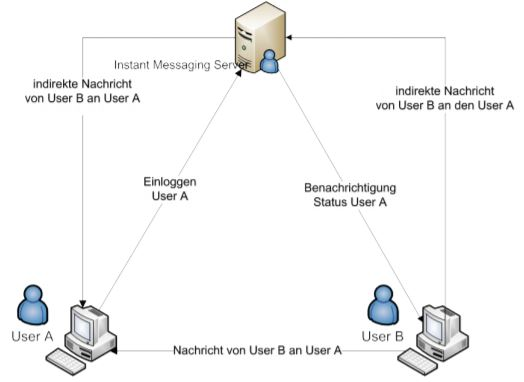
\includegraphics{images/GrundlegendeStrukturIMS}
	\caption{Allgemeine Struktur eines Instant-Messaging-Systems}
	\label{img:StrukturIMS}
\end{figure}

Hat sich der Benutzer mit seinen Login-Daten erfolgreich gegenüber dem Authentifikationsserver authentifiziert, kann er andere, bereits registrierte, Benutzer kontaktieren. Die Verbindungsinformationen wie zum Beispiel IP-Adresse, die dem Client lokal zugewiesene Portnummer und die Kontaktliste (Freunde des Benutzers) werden an den Präsenzserver übermittelt. Dieser ist abhängig von der Implementierungsform ein Teil des \textbf{IM-Servers} oder ein eigenständiger Server. Der Präsenzserver überprüft, welche Benutzer aus der Kontaktliste verfügbar und angemeldet sind. Der Server sendet dem Benutzer die Ergebnisse der Statusüberprüfung zurück. Ist einer der gewünschten Benutzer \glqq online\grqq (verfügbar) kann durch die Auswahl der entsprechenden Kennung eine Verbindung aufgebaut werden und der Nachrichtenaustausch kann beginnen. Das ist möglich, weil der Server dem Sender die IP-Adresse und die Ziel-Portnummer des Kommunikationspartners übermittelt. Die Nachrichten werden direkt zwischen den Clients übertragen oder über den Server zwischen den Kommunikationspartnern übermittelt. Die Art der Übertragung ist von System zu System je nach Realisierung unterschiedlich. Der Kommunikationspfad ist abhängig von der Architektur und dem verwendeten Protokoll. Eine Nachricht kann zentral über den Server vermittelt werden (vgl. \autoref{img:StrukturIMS}-indirekte Nachricht) oder nach dem Peer-to-Peer-Prinzip (vgl. \autoref{img:StrukturIMS}-direkte Nachricht) erfolgen. 

\section{XMPP-Extensible Messaging and Presence Protocol}
\label{sec:XMPP}
\ac{XMPP} bedeutet \textbf{Extensible Messaging and Presence Protocol}. Wird dieses ins Deutsche übersetzt, so entsteht die Bedeutung eines erweiterbares Nachrichten- und Anwesenheitsprotokoll. Eine Definition die \ac{XMPP} sehr gut beschreibt. \ac{XMPP} basiert auf \ac{XML}, welches eine Markup Sprache darstellt. Das Ziel von \ac{XMPP} war ein Protokoll für das Instant Messaging zu entwickeln. Laut dem RFC6120 lässt sich mittels \ac{XMPP} Daten zwischen zwei oder mehreren Netzwerkeinheiten nahezu in Echtzeit austauschen, welches als Vorteil für Sofortnachrichten bezeichnet werden kann. Diesbezüglich nutzt es das Internet und erlaubt den Usern Sofortnachrichten an andere Anwender innerhalb des Internets zu schicken. \ac{XMPP} lässt sich in viele verschiedene Funktionen aufteilen, weshalb der grundlegende Zweck ein anderes Ziel verfolgt. Im einfachsten Sinne ist die Idee von \ac{XMPP} den Austausch von kleinen Teilen strukturierter Daten (\glqq \ac{XML} stanzas\grqq) zwischen einem oder mehreren Netzwerkteilnehmern zu ermöglichen. Primär wird \ac{XMPP} mithilfe einer Client-Server-Architektur implementiert, bei der sich ein Client mit einem Server verbindet, um mit anderen Teilnehmern Daten auszutauschen. Anderseits kann es als Protokoll auch zwischen Servern fungieren. Daraus resultiert der Vorteil nahezu unabhängig von Betriebssystemen und Browsern zu sein. Wird die Client-Server-Architektur implementiert, so ist in der Regel der Ablauf definiert durch folgende Schritte: \cite{RFC6120} 
\begin{enumerate}
	\item Bestimmen der IP-Adresse und des Ports zu dem sich verbunden werden soll 
	\item Eine \ac{TCP} Verbindung öffnen/aufbauen
	\item Öffnen eines \ac{XML}-Streams über \ac{TCP}
	\item Optional: Verwendung von \ac{TLS} für die Verschlüsselung
	\item Verwendung des SASLs Frameworks für die Authentifizierung
	\item Eine Ressource an den \ac{XML} stream anbinden
	\item Austausch unbegrenzter \glqq \ac{XML} stanzas\grqq ()=> kleine Teile strukturierter Daten) mit anderen Netzwerkteilnehmern
	\item Schließen des \ac{XML} streams
	\item Schließen der \ac{TCP} Verbindung
\end{enumerate}
Die folgende \autoref{img:XMPPcommunication} zeigt den Start einer Kommunikation, wie im genannten Ablauf dargestellt, über \ac{XMPP} und den \ac{XML}-streams.

\begin{figure}[h]
	\centering
	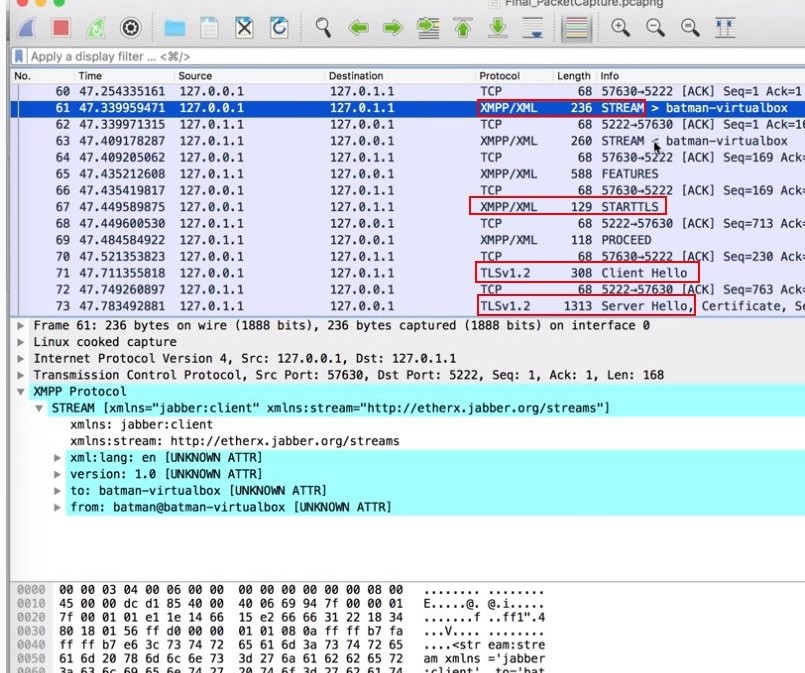
\includegraphics[width=\textwidth]{images/XML_Wireshark}
	\caption{Kommunikationsaufbau des \ac{XMPP}-Protokolls}
	\label{img:XMPPcommunication}
\end{figure} 
\newpage
Für den Austausch von Daten gibt es zwei elementare Konzepte. Zum einen die \ac{XML}-Streams und die \ac{XML}-Stanzas. Diese zwei Konzepte werden definiert um das Verständnis des Datenaustauschs, wie es im obigen Ablauf definiert ist, zu erlangen. Bei dem Austausch der Daten mittels \ac{XML} streams wird von einem Container zwischen den Teilnehmern gesprochen. Der \ac{XML} stream ist durch den \glqq stream header\grqq (z.B. \ac{XML} <stream>) und dem Ende des streams, dargestellt durch \ac{XML} </streams>, eindeutig definiert. Die Anzahl der austauschbaren \ac{XML} Elemente ist unbegrenzt und durch die Lebensdauer des streams definiert. Das \ac{XML} stanza wird nun als diskrete semantische Einheit strukturierter Daten, das von einem Teilnehmer zu einem anderen über den \ac{XML} stream gesendet wird bezeichnet. Das \ac{XML} stanza ist ein direktes Kind-Element des streams. Ein stanza kann wiederum selbst Kind-Elemente enthalten, das den \ac{XML} stream definiert. Im Kern fungiert der \ac{XML} stream wie eine Hülle um alle \ac{XML} stanzas, die während einer Session versendet werden. Ein Aufbau kann wie in der folgenden \autoref{img:StrukturXMLstream} repräsentiert werden. \cite{RFC6120Sec4}
\begin{figure}[h]
	\centering
	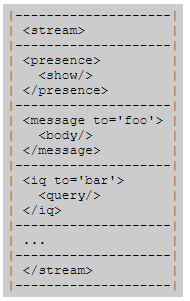
\includegraphics[scale=1.2]{images/XML_Stream}
	\caption{Allgemeine Struktur eines XML streams}
	\label{img:StrukturXMLstream}
\end{figure}
\newpage


\section{Grundlagen von Datenbanken}
\label{sec:Datenbank}
Für den Aufbau eines Chatsystems ist ein Datenbanksystem notwendig. Die Datenbank wird benötigt, weil Informationen und Parameter für die Authentifizierung des Benutzers gespeichert werden müssen. Außerdem ist die interne Datenbank Mnesia eines Ejabberd-Chatservers nicht für den Mehrbenutzer-Betrieb ausgelegt. Mnesia ist in der Sprache Erlang entwickelt. Sie besitzt eine weiche Echtzeitfähigkeit und ist auf Geschwindigkeit optimiert \cite{MnesiaDoc}. Die verfügbare Speicherkapazität von maximal 2 Gigabyte für den Betrieb ist nicht ausreichend für ein Mehrbenutzer-System \cite{ejabberdDoc}. Ein Mehrbenutzer-Betrieb eines ejabberd-Servers benötigt eine Datenbank, in der Nachrichtenverläufe, Kontakte jedes Benutzers und weitere Parameter gespeichert werden können.

\pagebreak

Eine Datenbank beinhaltet eine Sammlung von mehreren Daten, die sich aufeinander beziehen können, und von einem \ac{DBMS} verwaltet werden. Kernkomponente für den Zugriff ist die einheitliche logische Schnittstelle zum \ac{DBMS}. Der Zugriff kann mit dem weitverbreiteten Standard \ac{SQL}, welches im allgemeinen Sinn eine Programmiersprache darstellt, erfolgen. Dafür wird der Datenbank über \ac{SQL} nur mitgeteilt welche Daten benötigt werden. Ein Datenbanksystem muss bestimmte Eigenschaften besitzen, um den Zweck Daten zu speichern und sie wieder abzufragen, zu erfüllen.

\smallskip

\textbf{Eigenschaften:}
\begin{itemize}
	\item Unabhängigkeit von dem physischen Aufbau
	\item Schutz bei (Mehrfach-) zugriff auf Daten
	\item Integrität
	\item Zuverlässigkeit
	\item Ausfallsicherheit
\end{itemize}

Es gibt verschiedene Datenbankmodelle, nach denen eine Datenbankstruktur definiert wird. Die Datenbankmodelle unterteilen sich in relationale, objektorientierte, hierarchische und netzwerkartige sowie in moderne Datenbanken. Für die Projektarbeit wird ein relationales Datenbankmodell verwendet und deshalb dieses Modell genauer vertieft. Dementsprechend sind wichtige Schlüsselbegriffe zu definieren. Eine Tabelle wird ebenfalls als Relation bezeichnet. Eine Zeile der Relation heißt Tupel, die Spalten Attribute. Die Kardinalität entspricht der Anzahl von Tupeln und der Grad bezieht sich auf die Anzahl der Attribute. Ein wesentliche Bestandteil einer relationalen Datenbank ist der Primärschlüssel, welcher zwingend erforderlich ist und eindeutig sein muss. Der Schlüsselbegriff Gebiet bezieht sich auf ein Definitionsbereich eines Attributes, welches alle gültigen Werte für dieses Attribut umfasst. \cite{Schicker2017}

\newpage

\smallskip

\textbf{Beispiel einer Relation:}

\smallskip

\begin{figure}[h]
	\centering
	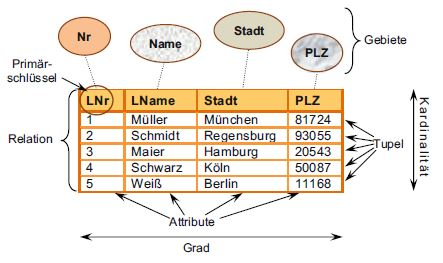
\includegraphics[scale=1.2]{images/RelationMitSchluesselbegriffe}
	\caption{Relation mit Schlüsselbegriffe \cite{Schicker2017}}
	\label{img:RelationDB_Begriffe}
\end{figure}

Eine relationale Datenbank ist definiert als eine Datenbank mit einer Ansammlung von zeitlich variierenden, normalisierten Relationen mit passenden Graden.
\textbf{MySQL} ist eines der weltweit verbreitetsten relationalen Datenbanksysteme, weil sie als Open-Source-Software und als kommerzielle Enterprise-Version verfügbar ist. MySQL wird von allen gängigen Betriebssystemen wie Linux oder Windows unterstützt. Entwickelt wird MySQL von der Oracle Cooperation. Die MySQL-Datenbanken sind relational und orientieren sich an den oben genannten Schlüsselbegriffen, die eine relationale Datenbank definieren. Die MySQL-Datenbank ist in der Software eine Client-Server-Architektur, die aus einem Multi-Threading-Server besteht. Dadurch werden verschiedene Backends, Clientprogramme und Verwaltungswerkzeuge parallel unterstützt.\cite{MysqlDoc}
\newpage

\section{Grafische Benutzeroberfläche}
\label{sec:Benutzeroberfläche}
Eine Grafische Benutzeroberfläche ist im Detail eine Schnittstelle zum Nutzer eines Computers. Die im Hintergrund agierende Software soll mittels Symbole und anderen Elementen bedienbar gemacht werden. Im Englischen wird die Benutzeroberfläche als \ac{GUI} bezeichnet, welches im weitere Verlauf ebenfalls als Bezeichnung verwendet wird. Allgemein besitzt eine \ac{GUI} Bedien- und Steuerelement die mit der im Hintergrund laufenden Software interagiert. Der Einsatz einer \ac{GUI} liegt an der Usability, welches die Benutzerfreundlichkeit beschreibt. Eine \ac{GUI} soll demnach dem User die Möglichkeit geben, die Software auch ohne großen Aufwand bedienen zu können. Eine Eigenschaft die heutzutage nahezu jedes Programm beinhalten muss. %TODO Quelle aendern
\url{https://de.wikipedia.org/wiki/Grafische_Benutzeroberfl%C3%A4che}
	
Im Rahmen der GUI-Programmierung müssen mehrere Aspekte berücksichtigt werden um die Usability zu erfüllen. Dafür werden die Aspekte in 8 goldene Regeln zusammengefasst, die bei der Entwicklung einer GUI berücksichtigt werden sollten.
\begin{enumerate}
	\item Strebe nach Konsistenz
	\item Sorge für universelle Bedienbarkeit
	\item Biete informative Rückmeldung
	\item Entwerfe abgeschlossene Dialoge
	\item Biete einfache Fehlerbehandlung
	\item Lass die Einfache Umkehrung von Aktionen zu
	\item Vermittle ein Gefühl der Kontrolle
	\item Entlaste das Kurzzeitgedächtnis
\end{enumerate}
Im Folgenden wird kurz auf die 8 Regeln eingegangen, damit eine Verbindung zur Umsetzung der \ac{GUI} in \autoref{subsec:EntwicklungGUI} entsteht.

Der erste Punkt, \textbf{Strebe nach Konsistenz}, befasst sich bspw. mit dem Erscheinungsbild einer Seite. Die Seite sollte dem Aspekt zur Folge die Elemente, wie einen Button, immer an der gleichen Stelle positionieren.

Der nächste Punkt, \textbf{Sorge für universelle Bedienbarkeit}, beinhaltet Anforderungen an die Vielfalt an Nutzer. Somit sollte jeder Nutzer die Bedienung, Kürzel usw. ohne Einschränkungen verstehen können.

Ein Nutzer verlangt nach ausreichendem Feedback, die vor allem informativ und in vielen Fällen auch hilfreich sind. Ein Fakt der im dritten Punkt, \textbf{Biete informative Rückmeldung}, behandelt wird

Der vierte Punkt, \textbf{Entwerfe abgeschlossene Dialoge}, umfasst die Führung eines Nutzers, bspw. durch eine Verkaufsprozess. Zu jedem Zeitpunkt soll der Nutzer wissen, in welchem Prozess er sich befindet.

Um die Bedürfnisse der Nutzer gerecht zu werden muss wie in Punkt fünf, \textbf{Biete einfache Fehlerbehandlung}, definiert, die Fehler mit nützlichen Informationen für den Nutzer ausgestattet werden. Außerdem muss ein Ausweg in den normalen Programmablauf gewährleistet sein.

Ein Nutzer soll mit Punkt sechs, \textbf{Lass die Einfache Umkehrung von Aktionen zu}, die Möglichkeit haben kleine Ereignisse rückgängig zu machen.

Der siebte Punkt, \textbf{Vermittle ein Gefühl der Kontrolle}, beinhaltet die Aktion und Reaktion. Demnach soll die Software auf eine Aktion des Nutzers reagieren und nicht andersrum. 

Der letzte Punkt, \textbf{Entlaste das Kurzzeitgedächtnis}, soll gewährleisten, dass die GUI schlicht und einfach gehalten werden soll. Ein Nutzer sollte sich keine große Anzahl an Informationen merken müssen um einen Aktion auszuführen.
\cite{UI8Regeln2019}

Aufgrund der 8 goldenen Regeln, kann im Umsetzungsprozess auf diese zurückgegriffen werden um eine benutzerfreundliche Oberfläche zu erstellen. Im folgenden Abschnitt wird auf die \ac{GUI}-Programmierung mit Python eingegangen.


\subsection{GUI-Programmierung mit Python}
\label{subsec:GuiPython}
Mit Python als Programmiersprache kommen mehrere Module, welche für die Grafische Benutzeroberfläche benutzt werden können, einher. Dementsprechend wird in diesem Abschnitt ein Einblick in die Möglichkeiten, passend zur Aufgaben- und Problemstellung, gegeben werden. Abhängig von den Erkenntnissen folgt eine Entscheidungsmatrix um das passende Modul für das Projekt auszuwählen.

Die \ac{GUI}-Programmierung bei Python unterscheidet sich im Konzept nicht allzu sehr von anderen Programmiersprachen. Neben Schaltflächen stehen auch Fenster oder Menüs als Komponenten zur Verfügung. Angeordnet können diese in sogenannten Container. Für eine geeignete Anwenderschnittstelle müssen die Komponenten in die Container integriert werden. Hinzukommt ein äußerer Container, auch als Frame bezeichnet, ein Layout-Manager und eine Implementierung damit Aktionen durch Komponenten ausgelöst werden können. Wie im \autoref{sec:Benutzeroberfläche} erläutert, verfolgt eine \ac{GUI} mehreren Regeln. Demnach gibt es für die Programmierung einer grafischen Benutzeroberfläche vielerlei Möglichkeiten. In Python werden \ac{GUI} Frameworks angeboten, die eine Programmierung erleichtern sollen. Diese Frameworks können sich in der Art und der Verwendung unterscheiden. Aufgrund davon muss erst die Art des Frameworks ermittelt werden. Dafür wird eine Entscheidungsmatrix erstellt, basierend auf Faktoren, die passend zum Projekt Auswirkungen haben.\cite{Steyer2018} \\
Die nachfolgende \autoref{tab:EntscheidungsmatrixFrameworkart} spiegelt die Ergebnisse eines Vergleichs zwischen den Tool-Frameworks und den Web-Frameworks von Python wieder. Die Kriterien orientieren sich am Projekt und werden nachfolgend erläutert. Die \textbf{Nutzerfreundlichkeit} umfasst wie verständlich ein GUI mithilfe des Tools aufgebaut werden kann. Außerdem beinhaltet das Kriterium auch die Möglichkeiten des Tools auf die Nutzerfreundlichkeit einzugehen. Die \textbf{Schwierigkeit} orientiert sich an der Implementierung. Dabei geht darum wie leicht, schnell und komfortabel die Frameart integriert werden kann. Unabhängig von der Schwierigkeit geht es bei der \textbf{Umsetzbarkeit} um die Mittel, welche für eine Umsetzung benötigt werden, sowie auch um den Aufwand bei der Umsetzung. Die \textbf{Kompatibilität} umfasst die Unabhängigkeit von Betriebssystemen, Browsern usw. Standard für eine grafische Oberfläche bildet auch das \textbf{Design}. Demnach geht es um die Möglichkeiten eines guten Erscheinungsbilds der Oberfläche mit dem entsprechenden Framework. Das letzte Kriterium, \textbf{Verwendungszweck}, bildet die Verbindung zum Projekt. Dabei wird analysiert wie die Frameworkart zum Zweck des Projektes passt. Die Gewichtung der Kriterien innerhalb der \autoref{tab:EntscheidungsmatrixFrameworkart} sind der TABELLE des ANHANGS zu entnehmen. %TODO Tabelle in den Anhang packen
\renewcommand{\arraystretch}{2}
\begin{table}[h]
\centering
	\begin{tabular}{l|c|c|c}
		& & \multicolumn{2}{c}{Arten einer Python-GUI} \\
		Kriterien & Gewichtung & Tool-Framework & Web-Framework \\
		\hline
		Nutzerfreundlichkeit & 33\% & 2 & 2 \\
		\hline
		Schwierigkeit & 7\% & 2 & 1,7  \\
		\hline
		Umsetzbarkeit & 13\% & 2 & 2,2\\
		\hline
		Kompatibilität & 13\% & 2,2 & 1,7 \\
		\hline
		Design & 7\% & 2 &  2\\
		\hline 
		Verwendungszweck & 27\% & 2,5 & 1,5 \\
		\hline
		\textbf{Gesamtwertungszahl} & \textbf{100\%} & \textbf{2,161} & \textbf{1,831} \\
	\end{tabular}
\caption{Entscheidungsmatrix der Frameworkart} %TODO Tabellen caption über die Tabelle positionieren
\label{tab:EntscheidungsmatrixFrameworkart}
\end{table} \\
Die \autoref{tab:EntscheidungsmatrixFrameworkart} bildet eine Hilfestellung zur Entscheidung einer passenden Frameworkart für das Projekt. Die Bewertung der Tools entsprechend der Kriterien folgt dem Benotungsschema der akademischen Bildung. Demnach ist eine 1 sehr gut und eine 6 ungenügend. Im Kriterium Nutzerfreundlichkeit schließen beide Frameworks mit der gleichen Note ab, da die Nutzerfreundlichkeit abhängig vom Designstil ist und bei beiden Frameworks umgesetzt werden kann. Die Schwierigkeit, wie das Kriterium in der Einführung definiert wurde, bekommt beim Web-Framework eine bessere Bewertung. Grund hierfür ist, dass für das Web-Framework überwiegend keine aufwändigen Module in Python benötigt werden. Die Gestaltung erfolgt nämlich über HTML und CSS, welche dann mit einem schlichten Modul verknüpft bzw. aufgerufen werden können. Aufgrund von Vorkenntnissen sowohl in HTML als auch in CSS wird die Schwierigkeit für das Web-Framework besser bewertet. Bei der Umsetzbarkeit steht das Tool-Framework aufgrund der Verwendung eines gesamten Moduls besser da. Ein Web-Framework bringt HTML, CSS und das Modul mit was ein größeren Umfang bedeutet. Vor allem muss der Programmierer mit allen Elementen umgehen können, weshalb eine Umsetzung schwieriger sein könnte. In der Kompatibilität wird das Web-Framework aufgrund der Unabhängigkeit bezüglich des Betriebssystem besser bewertet. Außerdem kann eine ausgelieferte HTML-Seite von nahezu allen Browsern gelesen werden, und eine Möglichkeit die Lösung auf mobilen Endgeräten zu benutzen ist ebenfalls enthalten. Im Design unterscheiden sich die Frameworkarten nicht. Beide bieten vielerlei Möglichkeiten im Bezug auf die Gestaltung. Aufgrund des Projektes einen Chat über \ac{XMPP} und ejabberd zu realisieren wird schon hauptsächlich das Internet genutzt. Dadurch bietet es sich den Server eine HTML-Seite ausliefern zulassen. Aus diesem Grund wird das Web-Framework im Rahmen dieses Kriteriums besser bewertet. Anhand der Gesamtwertungszahl entsprechend der Benotung und der Gewichtung sind beide Frameworks zu empfehlen, dennoch schließt das Web-Framework besser ab, weshalb im weiteren Verlauf ein Web-Framework zum Einsatz kommen soll. \cite{FrameworkOverview} \cite{WebFramework}\\
Mit diesem Ergebnis müssen die verschiedenen Möglichkeiten eine Web-Framework in Bezug auf Python analysiert und bewertet werden. Auch in diesem Fall liefert eine Entscheidungsmatrix ein aufschlussreiches Ergebnis. Die Definition der selben Bewertungskriterien sind der Einführung der \autoref{tab:EntscheidungsmatrixFrameworkart} zu entnehmen. Kriterien wie Umfang und Komplexität werden in die Betrachtung miteinbezogen. Der \textbf{Umfang} spiegelt die Möglichkeiten und Größe im Aufbau des Tools wieder. Die \textbf{Komplexität} befasst sich im Grunde mit dem Aufwand einer Implementierung sowie auch die Hilfestellungen durch geeignete Dokumentationen. Das Bewertungsschema orientiert sich ebenfalls an der \autoref{tab:EntscheidungsmatrixFrameworkart}.\\
\begin{table}[h]
	\centering
	\begin{tabular}{l|c|c|c|c|c}
		Kriterien & Gewichtung & Django & Flask & CherryPy & Bottle\\
		\hline
		Umfang & 17\% & 1,5 & 2 & 2 & 2,5 \\
		\hline
		Schwierigkeit & 17\% & 2,5 & 1,7 & 2,2 & 2 \\
		\hline
		Komplexität & 33\% & 2,2 & 1,7 & 2 & 1,7 \\
		\hline
		Verwendungszweck & 33\% & 2 & 2 & 2 & 2,2 \\
		\hline
		\textbf{Gesamtwertungszahl} & \textbf{100\%} & \textbf{2,067} & \textbf{1,850} & \textbf{2,033}  & \textbf{2,050} \\
	\end{tabular}
	\caption{Entscheidungsmatrix eines Web-Frameworks}
	\label{tab:EntscheidungsmatrixWebFramework}
\end{table}Die Gesamtwertungszahl, welches der \autoref{tab:EntscheidungsmatrixWebFramework} entnommen werden kann, liefert ein knappes Ergebnis. Demnach bietet sich Flask am besten als Framwork einer grafischen Oberfläche an. Im Umfang setzt sich das Tool Django gegen die Konkurrenten durch, da es aufgrund seiner Größe vielerlei Möglichkeiten mitbringt. Während die anderen Tools überwiegend als Mikroframework bezeichnet werden zeichnet sich Django als Full-Stack/high-level Framework aus. Ebenfalls ein Grund weshalb die Schwierigkeit bei Django mit einer 2,5 bewertet wurde. Ein Mikroframework bildet in der Hinsicht die leichtere und schnellere Variante. Die Komplexität wurde vor allem bei Flask und Bottle gut bewertet. Grund hierfür ist unter anderem eine geringere Komplexität durch Möglichkeiten einer schlichten Implementierung. Außerdem bietet bspw. Flask eine sehr gute Dokumentation, welche die Komplexität verringern. Der Verwendungszweck ist nahezu gleichbleibend, da alle Frameworks genutzt werden können um das Projekt umzusetzen. Ausschließlich bei Bottle ist überwiegend die Rede von einem Framework das vor allem zur Einführung in das Themengebiet der Programmierung grafischer Oberflächen mit eine Web-Framework benutzt wird. Anhand des Ergebnisses und der sehr guten Dokumentation wird Flask als Web-Framework zum Einsatz kommen.\cite{BottleDoc} \cite{CherryPyDoc} \cite{DjangoDoc} \cite{FlaskDoc}

\subsection{Flask}
\label{subsec:Flask}
Wie unter \autoref{subsec:GuiPython} beschrieben, wird im Rahmen der Studienarbeit Flask verwendet. Es ist ein Python Web-Framework welches eine Schnittstelle zum Webserver bildet. Bekannt ist Flask durch die Eigenschaft schnell und leicht eine minimale Anwendung zu implementieren und diese bei Bedarf in der Größe zu skalieren. Für die Verwendung von Flask sind zwei Bibliotheken wichtig. Bei diesen handelt es sich zum einen über die \ac{WSGI}-Bibliothek Werkzeug und der Template-Bibliothek Jinja2. Module die standardmäßig von Flask verwendet werden. Flask bildet im Grunde das Bindeglied zwischen den Modulen und erlaubt es bspw. mithilfe des \textbf{Routings} an bestimmten Endpunkten eine \ac{HTML}-Datei zu rendern. Ein Möglichkeit dafür zeigt das folgende \autoref{lst:FlaskMinApp}.
\begin{lstlisting}[language=Python,caption=Example Listing of Flask Python,label={lst:FlaskMinApp}]
from flask import Flask
app = Flask(__name__)

@app.route('/')
def homepage():
	 return render_template('homepage.html')
\end{lstlisting}
Das \autoref{lst:FlaskMinApp} spiegelt das Routen sowie das Rendern einer \ac{HTML}-Datei von Python wieder. Aufgrund des Paketverwaltungsprogramm pip kann Flask komfortable installiert werden. Dementsprechend wird Flask in der ersten Zeile importiert, dann einer Anwendung zugeordnet und eine Route definiert. Nun besitzt Flask vielerlei Möglichkeiten, so kann bspw. je nach Anfrage (POST, GET, usw.) differenziert werden. In dem Zusammenhang kommt eine weiterer möglicher Vorteil von Flask zum Einsatz. Dieser beinhaltet die Möglichkeit einen Webserver, den Flask zur Verfügung stellt, im Entwicklungsmodus zu starten und aktuelle Code-Zeilen zu testen.
Flask ist also nicht zuständig für die Gestaltung der grafischen Oberfläche sondern benutzt sogenannte \textbf{Templates} in Form von HTML-Datei, die eine Webseite aufbauen. Für eine dynamische Webanwendung und den gestalterischen Aspekten sind statische Dateien, wie z.B. \ac{CSS}, notwendig. Aus diesem Grund benötigt Flask eine vorgegebene Ordnerstruktur, welche der nachfolgenden \autoref{img:TreeFlaskOrdnerstrukt} entnommen werden kann.
\begin{figure}[h]
	\centering
	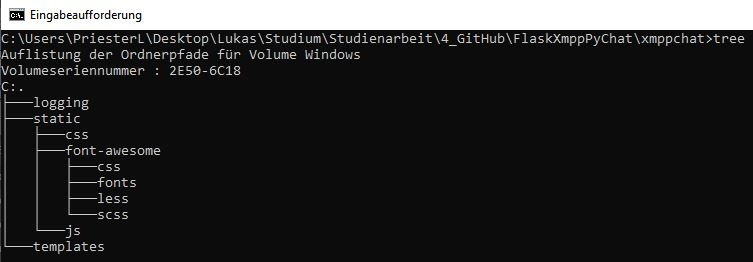
\includegraphics[width=\textwidth]{images/TreeFlaskOrdnerstrukt}
	\caption{Ordnerstruktur unter Flask, eigene Darstellung}
	\label{img:TreeFlaskOrdnerstrukt}
\end{figure}
Für die grafische Benutzeroberfläche würden diese Elemente ausreichen um eine simple Webseite aufzubauen, mit den \ac{HTML}- und \ac{CSS}-Dateien zu verknüpfen, über das Routen die Seite zu rendern und letztendlich, über den von Flask gestellten Webserver, zu testen. Dennoch bietet Flask mehr Möglichkeiten auch im Zusammenhang des Projektes. Zum Beispiel kann in Flask mit redirects, sessions, cookies, Datenbanken und vieles mehr gearbeitet werden. Dabei verfolgt Flask das Ziel dem Anwender nichts vorzuschreiben, dadurch ist er unabhängiger und kann auf vielerlei Erweiterungen zugreifen. Bei der Anbindung einer \textbf{Datenbank} gibt es so die Möglichkeit bspw. eine MySQL, PostgreSQL, SQLite oder andere Datenbanken zu verwenden. In diesem Zusammenhang bietet Flask das Modul Flask-SQLAlchemy, welches der Flask-Anwendung das SQLAlchemy Paket hinzufügt. Ziel ist es die Verwendung von SQLAlchemy mit Flask zu vereinfachen. Das Paket gilt als \ac{ORM}, und bietet die Möglichkeit high-level Operationen in Datenbank-Kommandos zu übersetzen. Im Rahmen der Studienarbeit wird ebenfalls die Erweiterung Flask-SQLAlchemy angewendet. Demnach kann eine Implementierung, einer minimalen Anwendung mit Datenbank, wie im folgenden \autoref{lst:SQLAlchemyMinApp} dargestellt, aussehen.
\begin{lstlisting}[language=Python,caption=Example Listing of Flask-SQLAlchemy,label={lst:SQLAlchemyMinApp}]
from flask import Flask
from flask_sqlalchemy import SQLAlchemy

app = Flask(__name__)
app.config['SECRET_KEY'] = os.urandom(24) #secret key of app
app.config['SQLALCHEMY_DATABASE_URI'] = config.get('SQLALCHEMY_DATABASE_URI')

db = SQLAlchemy(app)

class User(db.Model):
	user_id = db.Column(db.Integer, primary_key=True, autoincrement=True)
	username = db.Column(db.String(25), unique=True, nullable=False)
	email = db.Column(db.String(35), unique=True, nullable=False)
	passwd = db.Column(db.String(112), nullable=False)
	
	def __init__(self, user, email, passwd):
		self.username = user
		self.email = email
		self.passwd = self.set_password(passwd)
	
	def get_id(self):
		return (self.user_id)

@app.route('/login')
def login():
	user = User(req_content["username"], req_content["eMail"], req_content["password"])
	db.session.add(user)
	db.session.commit()
	return render_template('homepage.html')
\end{lstlisting}
Neben dieser Erweiterung bietet Flask auch ein Modul im Rahmen eines Login, welcher ebenso für das Projekt relevant ist, an. Dafür kann der Login Manager aus Flask-Login verwendet werden. Dieser beinhaltet nützliche Funktionen auf die innerhalb der Anwendung zugegriffen werden kann. Für den Login-Manager werden sessions benötigt, welche ebenfalls importiert werden müssen. Das liegt an der Authentifizierung, weshalb ein sicherer Schlüssel, wie er im \autoref{lst:LoginManagerMinApp} dargestellt ist, erzeugt werden muss.
\begin{lstlisting}[language=Python,caption=Example Listing of Flask-Login,label={lst:LoginManagerMinApp}]
from flask import Flask
from flask_login import LoginManager, login_required, login_user, logout_user, current_user

app = Flask(__name__)

login_mgmt = LoginManager(app)
login_mgmt.login_view = 'login' # name of callback method if unauthorized user accessed a login protected site

@app.route("/login", methods=['GET', 'POST'])
def login():
	if current_user.is_authenticated:
		return redirect(url_for('gochat'))
	login_user(user)
	return render_template('login.html')
\end{lstlisting}
Diese beispielhafte Listings wichtiger Module zeigen die Möglichkeiten des Web-Frameworks. Mitunter der Grund für die Verwendung von Flask. Außerdem sind nur wenige Module dargestellt. Weitere Erweiterungen, die im Rahmen des Projektes eingesetzt werden folgen bei der Umsetzung. Diese dargestellt bilden lediglich die theoretische Grundlagen um das Funktionsprinzip von Flask zu erläutern.
\pagebreak

\section{HTML, CSS und JavaScript als Werkzeuge der Webentwicklung}
\label{sec:HTMLCSSJS}
Wie unter \autoref{subsec:Flask} erläutert, benötigt Flask für die grafische Oberfläche weitere Elemente, die das Erscheinungsbild aufbauen, gestalten und mit Dynamik verknüpfen. Dafür werden die Werkezeuge des Webdesign benötigt. Diese umfassen \ac{HTML}, \ac{CSS} und JavaScript.

\textbf{\ac{HTML}}\\
Das Internet mit seinen Funktionen Text-, Bild, Sound und weiteres abzubilden oder zu übertragen basiert auf einem gemeinsamen Standard. Dieser ist unter dem Namen Hypertext Markup Language \ac{HTML} bekannt, welcher zu deutsch unter einer Auszeichnungssprache zu verstehen ist. Konkret bezieht sich HTML auf Hypertexte die per Definition die Verlinkung zwischen Texte mithilfe von Hyperlinks bezeichnen. \ac{HTML} als Markup Language entstand schon 1989 und diente zur Beschreibung und Verlinkung von Text. Mit \ac{HTML}5, welches ergänzend zur ersten Variante auch Audio- oder Videodateien an die Webseite binden kann, befindet sich die aktuellste Version im Umlauf. Während eine Weboberfläche unabhängig vom Betriebssystem ist, spielt die Verwendung von Browsern, die ihre eigenen HTML-Parser besitzen, eine bedeutsame Rolle. Aus diesem Grund können vom Webserver ausgelieferte \ac{HTML}-Dateien bei einer geringen Anzahl an Browsern Probleme bereiten. Innerhalb eines \ac{HTML}-Dokuments ist vor allem das Grundgerüst und der Aufbau relevant. Demnach werden die Elemente einer Webseite mit Sprachelementen, sogenannten Tags, beschrieben. Der Aufbau eines Grundgerüst ist in der \autoref{img:GrundgeruestHTML} dargestellt.
\begin{figure}[h]
	\centering
	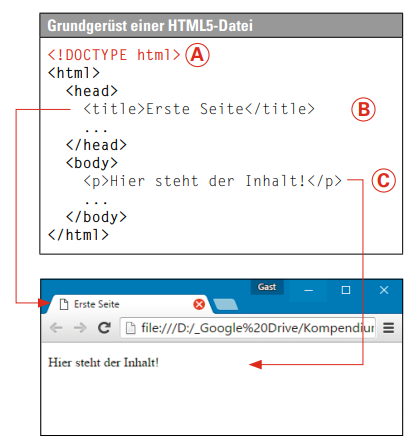
\includegraphics[scale=1.3]{images/HTML_Grundgeruest}
	\caption{Grundgerüst einer HTML-Datei, \cite{buhler2017html5}}
	\label{img:GrundgeruestHTML}
\end{figure}
\\Der \autoref{img:GrundgeruestHTML} sind die 3 wichtigen Tags (html, head, body) eines Standard \ac{HTML}-Dokumentes sowie der unter A angegebenen Dokumenttyp zu entnehmen. Während in vielen Programmiersprachen die Syntax umfassend groß sein kann, ist die Grammatik bei HTML sehr schlicht. Für die Korrektheit sind daher die genannten Tags bedeutend. Außerdem werden überwiegend Verschachtelung bei der Darstellung einer Webseite benötigt. Für weiteren Einfluss auf die Tags können sogenannte Attribute, wie in der folgenden \autoref{img:HTMLattribute} dargestellt, den Tags zugeteilt werden. 
\begin{figure}[h]
	\centering
	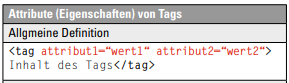
\includegraphics[scale=2.5]{images/HTMLattribute}
	\caption{Attribut eine \ac{HTML}-Tags, \cite{buhler2017html5}}
	\label{img:HTMLattribute}
\end{figure}
\\Eine \ac{HTML}-Datei entsteht also vor allem durch Tags. Während nun das Dateiformat als reine Textdatei vorliegt, entstehen Fragen über die gestalterischen Aspekte wie z.B. Farben, Grafiken, Videos oder ähnliches. Hauptsächlich werden diese Aspekte innerhalb einer \ac{CSS}-Datei behandelt, dennoch gibt es dafür auch Punkte, die in einer \ac{HTML}-Datei zu beachten sind. Um beispielsweise Grafiken oder Videos, die sich innerhalb eines anderen Unterordners befinden, zu integrieren, muss auf diese referenziert werden. Hierfür bietet \ac{HTML} die absolute und relative Referenz. Eine absolute Referenz, wie z.B. \textit{C:/Dokumente/Mustermann/ Eigene Dateien/Webseiten/button.gif}, wird aufgrund der Abhängigkeit zum User des Computers nicht verwendet. Für die relative Referenz ist wiederum eine einheitliche Ordnerstruktur wichtig, da der Pfad von dem Speicherort der \ac{HTML}-Datei angegeben wird. Diese Struktur kann, wie in der folgenden Abbildung dargestellt, aussehen.
\begin{figure}[h]
	\centering
	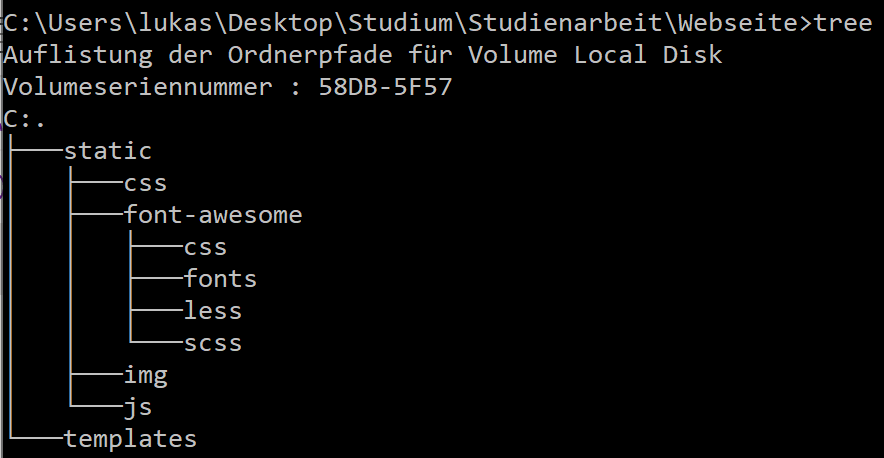
\includegraphics[scale=0.8]{images/TreeHTMLStruktur}
	\caption{Ordnerstruktur bei der Webentwicklung, eigene Darstellung} 
	\label{img:TreeHTMLStruktur}
\end{figure}
\\Demnach würde die \ac{HTML}-Datei in dem Ordner \textit{templates} liegen und die Bilder im Ordner \textit{static/img}, welcher über die relative Referenz unabhängig vom Betriebssystem und ähnliches erreicht werden kann. Je nach Dateityp orientieren sich auch die Tags innerhalb des \ac{HTML}-Dokumentes danach. Für eine Grafik gibt es daher den <img>-Tag, der die Referenz zum Bild enthält. Mit der Webentwicklung wird das Ziel verfolgt Inhalt und Gestaltung strikt voneinander zu trennen. Daher werden \ac{CSS}-Dateien, die sich mit dem Design befassen, benötigt.

\textbf{CSS:}\\
Die Dateien, die als \ac{CSS} deklariert werden, übernehmen die gestalterischen Aspekte, die ein \ac{HTML}-Dokument nicht erfüllen kann. Neben Designvarianten bietet \ac{CSS} auch die Möglichkeit die Webseite an das jeweilige Endgerät, unterschiedlicher Auflösung, anzupassen. Wie schon für die \ac{HTML}-Dateien gilt auch für \ac{CSS}, dass Attribute nur von bestimmten Browsern akzeptiert werden. Daher gehört zur Webentwicklung ein ausgiebiges Testen dazu. Eine \ac{CSS}-Datei sollte Regeln folgen um Probleme, die im Zusammenhang mit dem HTML-Dokument auftreten können, zu verhindern. Die Grundregel bezieht sich auf den Ort der \ac{CSS}-Definition. Diese kann zum Einen in einer externen Datei, intern in einem eigenen Tag, oder integriert in den \ac{HTML}-Tag erfolgen. Dies ist unter anderem relevant wenn mehrere \ac{CSS}-Dateien zum Einsatz kommen, da die verschieden Orte durch verschiedene Prioritäten geprägt sind. Generell wird die \ac{CSS}-Definitionen in eine eigene Datei ausgelagert um das Design und die \ac{HTML}-Datei zu trennen. Die \autoref{img:CSSrules} stellt dar wie eine \ac{CSS}-Definition aufgebaut ist.
\begin{figure}[h]
	\centering
	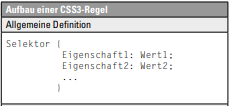
\includegraphics[scale=2.5]{images/CSS_Definition}
	\caption{Aufbau einer \ac{CSS}-Regel, \cite{buhler2017html5}}
	\label{img:CSSrules}
\end{figure}	
\\Der Aufbau besteht grundlegend aus einem Selektor, dem seine Eigenschaften bearbeitet werden sollen. Damit die Auswirkungen erkennbar werden muss die \ac{CSS}-Datei mit dem HTML-Dokument verknüpft werden. Dies erfolgt innerhalb des Head-Tags in der \ac{HTML}-Datei mithilfe des link-Tags \textit{<link rel=\dq sytlesheet\dq \;type=\dq text/css\dq \;href=\dq design.css\dq>}. Der Selektor befindet sich immer vor einer geschweiften Klammer und kann unterschiedlich verwendet werden. Aufgrund der Verbindung zur HTML-Datei hängt der Selektor vom \ac{HTML}-Tag ab. Wird bspw. ein Button in dem \ac{HTML}-Tag als Klasse definiert so erfolgt der Zugriff über den Punkt. Wird jedoch der Button mit einer ID ausgestattet, so muss mit dem Hashtag darauf zugegriffen werden. Die nachfolgende Abbildung zeigt diese Varianten.
\begin{figure}[h]
	\begin{minipage}[c]{.4\textwidth}
		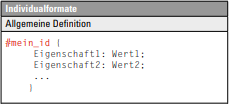
\includegraphics[width=\textwidth]{images/CSSID}
		\caption{Zugriff über ID, \cite{buhler2017html5}} 
		\label{img:CSSID}
	\end{minipage}
	\hspace{.1\linewidth}% Abstand zwischen Bilder
	\begin{minipage}[c]{.4\textwidth}
		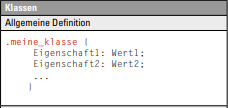
\includegraphics[width=\textwidth]{images/CSSKlasse}
		\caption{Zugriff über Klasse, \cite{buhler2017html5}} %TODO richtige Größe
		\label{img:CSSClass}
	\end{minipage}
\end{figure}
Für die Eigenschaften bietet sich mit der dritten Version von \ac{CSS} (\ac{CSS}3) eine Vielzahl an Möglichkeiten. Grundlegend kann jedes Element mithilfe der \ac{CSS}-Datei bearbeitet werden. Die Eigenschaften sind bspw. Gegliedert unter Typografie, Farbe, Abstände, Tabellen und vieles mehr. In diesem Zusammenhang ist auch die Verwendungen von Maßeinheiten bedeutsam. Mit \ac{CSS}3 werden viele verschiedene Ma"seinheiten unterstützt worüber die Abbildung einen genaueren Überblick gibt.
\begin{figure}[h]
	\centering
	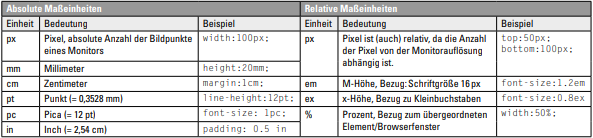
\includegraphics[scale=1.8]{images/CSSmasseinheiten}
	\caption{Ma"seinheiten innerhalb der Webentwicklung, \cite{buhler2017html5}} 
	\label{img:CSSmasseinheiten}
\end{figure}
\ac{CSS} verwendet die Selektoren und wendet auf diesen die definierten Eigenschaften an. Nebenbei bietet \ac{CSS} die Möglichkeit an ein Layout zu erstellen. Dafür ist das sogenannte Boxmodell ausschlaggebend. Dieser ist definiert, die Elemente als eine Box mit Eigenschaften zu betrachten. Demnach gibt es in dem Zusammenhang vielerlei Möglichkeiten eine Box an die richtige Position, sowie mit der richtigen Größe abzubilden. Die Boxen können mit absoluten Werten definiert werden. Mit relativen Werten, welche Prozentwerte enthalten, können die Boxen sich in Abhängigkeit des Browserfensters ändern. Mit \ac{CSS}3 gibt es auch die Möglichkeiten flexible Boxen zu verwenden. Dadurch werden die Boxen unabhängig von der Position und Anordnung spalten- oder zeilenweise an den zur Verfügung gestellten Platz angeordnet. Bei der Betrachtung des Layouts spielt ebenfalls das Endgerät eine Rolle. In dem Zusammenhang können \textbf{Media Queries} zum Einsatz kommen. Diese bieten die Option, Eigenschaften eines Selektors entsprechend der angegebenen Pixel zu ändern.
\begin{figure}[h]
	\centering
	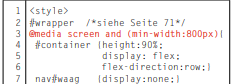
\includegraphics[scale=2.8]{images/MediaQbsp}
	\caption{Beispiel eines Media Queries, \cite{buhler2017html5}}
	\label{img:/MediaQbsp}
\end{figure}
\\Die Abbildung stellt dar wie die Media Queries eingesetzt werden können. Die Definition erfolgt entweder in der \ac{CSS}-Datei oder in dem Style-Tag einer \ac{HTML}-Datei. Mit diesen Grundlagen lassen sich Seiten gestalterisch anpassen und auf mehreren mobilen Endgeräten ausgeben. Wird Content benutzt der sich ggf. zur Laufzeit ändert, wird überwiegend auf das dritte Element der Webentwicklung zurückgegriffen. Dabei geht es um JavaScript.\cite{buhler2017html5}

\textbf{JavaScript}\\
JavaScript verfolgt das Ziel interaktive oder dynamische Elemente auf der Webseite zu integrieren. Es ist eine Skriptsprache, die überwiegend auf Seiten des Clients eingesetzt wird. Der Code kann direkt über den Browser ausgeführt werden, da ein heutiger Browser einen Interpreter für die Skriptsprache besitzt. Dadurch ist JavaScript von den heutigen Browsern abhängig, weshalb ausgiebige Tests auf verschiedene Browsern erfolgen muss. Mit JavaScript ergeben sich Möglichkeiten Probleme bzw. Schwierigkeiten dynamisch zu lösen. Ein beliebter Fall als Beispiel ist die Formularüberprüfung. Hierbei kann JavaScript die Korrektheit noch auf Seiten des Clients überprüfen und erst nach Abschluss dem Server übertragen. Dadurch können unnötige Datenübertragungen verhindert werden. Eine Schwierigkeit die JavaScript birgt ist die Ausschaltfunktion in den meisten Browsern. Besitzt eine Webseite eine große Anzahl an JavaScript Code so kann durch Deaktivierung im Browser mancher Content nicht mehr funktionieren. Wie mit der Integration von CSS gibt es auch bei JavaScript die Möglichkeit es innerhalb der HTML-Datei oder in einer externen Datei zu verwenden. Im Falle der internen Lösung gibt es den <script>-Tag, der eine JavaScript-Code enthalten kann. Das nachfolgende \autoref{lst:JavaScriptExample} stellt dar, wie so ein JavaScript in den HTML-Body integriert werden kann.
\begin{lstlisting}[language=HTML,caption=Example Listing of JavaScript-Code,label={lst:JavaScriptExample}]
<div class="Login_succeeded">
<script>
document.write("Your Login was succesful");
</script>
</div>
\end{lstlisting}
Das Beispiel bildet ein simpler Fall von JavaScript ab. Der Code erzeugt lediglich ein Text in der HTML-Klasse. Eine der beliebtesten Verwendungen von JavaScript sind Fenster, die zur Benachrichtigung oder Warnung benutzt werden. In Verbindung mit Event-Handler, die auf bestimmte Ereignisse reagieren, kann so, je nach Anwendung Fenster oder andere Elemente erzeugt werden. Ein Beispiel für solch ein Event-Handler wäre das "onclick". Dadurch lässt sich JavaScript-Code erst ausführen wenn bspw. auf ein Button geklickt wird. Neben Fenstern gibt es zahlreiche weitere Verwendungsmöglichkeiten, wie zum Beispiel Formulare, Textfelder, Checkboxen usw. Eine besondere Variante von JavaScript ist \textbf{\ac{Ajax}}, welches ein weiteres wichtiges Feature mit in die Webentwicklung einbringt. \ac{Ajax} kommt vor allem zum Einsatz, wenn es um Elemente geht die nicht durch eine Aktualisierung des Browser ausgelöst werden sollen. \ac{Ajax} ermöglicht in solch einem Fall die dynamische Anfrage. Die Nachfolgende \autoref{img:/AjaxUseCase} erklärt das Funktionsprinzip von \ac{Ajax} sehr genau.
\begin{figure}[h]
	\centering
	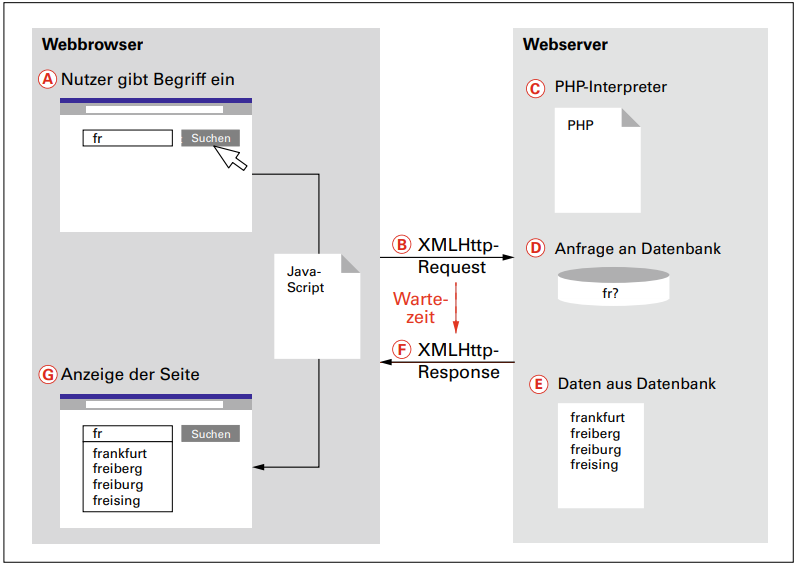
\includegraphics[scale=1.0]{images/AjaxUseCase}
	\caption{Anwendungsfall von Ajax, \cite{buhler2018webtechnologien}} 
	\label{img:/AjaxUseCase}
\end{figure}
Während ein User ein Textfeld beschreibt wird im Hintergrund, mithilfe des JavaScript-Objektes XMLHttpRequest, eine Anfrage an den Webserver gesendet. Dieser kann mit ersten Teilergebnissen antworten und so dem User bspw eine Autovervollständigung anbieten. Ajax ist in dem Fall keine neue Technologie sondert verwendet JavaScript anders um mit dem Webserver im Hintergrund zu kommunizieren. In diesem Fall ist die Autovervollständigung lediglich ein einfaches Beispiel um die Funktion von \ac{Ajax} zu verstehen. Darüber hinaus gibt es weitaus mehr Anwendungsfälle von \ac{Ajax}. Bei aufwändigen Webseiten kommt ein weiteres Element zur Webentwicklung hinzu, das die Entwicklung erleichtern soll. Dabei handelt es sich um Frameworks. Wie es für \ac{CSS} Bootstrap als Framework gibt, so werden viele auch im Zusammenhang mit JavaScript angeboten. Eines der beliebtesten Frameworks ist \textbf{jQuery}. Mit jQuery wird das Programmieren von JavaScript unterstützt. Außerdem orientiert es sich an der Darstellung von \ac{CSS} wie bspw. der Zugriff auf ein Element über \$(\dq \#bereich1\dq) oder \$(\dq .farbe1\dq). Wie JavaScript kann auch jQuery auf die Elemente der \ac{HTML}-Seite zugreifen. Der Standardaufbau, welcher in dem folgenden \autoref{lst:jQueryExample} dargestellt ist, zeigt eine Merkmal auf das zu achten ist.
\begin{lstlisting}[language=HTML,caption=Example Listing of jQuery,label={lst:jQueryExample}]
<script> $(document).ready(function(){
/* Hier der jQuery-Code */ });
</script>
\end{lstlisting}
Mit \textit{\$(document).ready} werden grundsätzlich erste Probleme, die auftreten können verhindert. Demnach könnte ohne diese Funktion auf Elemente zugegriffen werden, welche noch nicht vollständig geladen sind. Das ready verhindert diese Problematik und wartet mit der Ausführung bis die Webseite komplett geladen ist. JQuery besitzt zahlreiche Plugins die bei der Webentwicklung verwendet werden können. JavaScript bildetet ein fundamentaler Baustein, der mithilfe zahlreicher Möglichkeiten und Frameworks für jede Anwendung Optionen bereitstellt, um dynamische Änderungen oder Interaktionen zu integrieren.\cite{buhler2018webtechnologien}


\pagebreak
\section{Grundlagen von Softwaretests}
\label{sec:GrundlagenSoftwaretests}

Die Entwicklung eines Softwareprodukts ist stets aufwendig und fehlerbehaftet. Es gibt eine Reihe potentieller Fehler, die eine Software aufweisen kann.

\smallskip

\subsubsection*{Häufige Fehlerarten:}

\smallskip

\begin{itemize}
\item syntaktische Fehler
\item semantische Fehler
\item Logische Fehler
\item Designfehler
\item Fehler im Bedienkonzept
\item Laufzeitfehler
\item Fehler als Folge physikalischer Betriebsbedingungen
\end{itemize}

Syntaktische Fehler verstoßen gegen die Richtlinien und der Grammatik der Programmiersprache. Bei semantischen Fehlern ist die Syntax korrekt, aber das Programm ist inhaltlich falsch. Ein Beispiel wäre eine falsche Parameterreihenfolge in einer Funktion. Logische Fehler bestehen aus einem falschen Problemlösungsansatz, zum Beispiel aufgrund eines Fehlschlusses oder einer falschen Interpretation einer Programmspezifikation. Designfehler sind Fehler im Grundkonzept der Software. Die Ursachen liegen in der Definition der Anforderungen an das Softwareprodukt oder an Codewiederholungen, die bei Software-Wartungen nicht auf den gleichen Stand gebracht werden. Ein Fehler im Bedienkonzept ist ein Fehler, bei dem sich das Programm anders als von Benutzern erwartet verhält, obwohl es technisch fehlerfrei arbeitet. Laufzeitfehler sind Fehler, die auftreten während das Programm abgearbeitet wird. Ein möglicher Laufzeitfehler entsteht durch einen Aufruf eines Unterprogramms mit falschen Eingabeparametern. Fehler als Folge physikalischer Betriebsbedingungen sind Fehler, die durch elektromagnetische Felder, Temperaturschwankungen oder Strahlung bei technisch einwandfreier Software zu Fehlern und unerwünschten Verhalten führen. Ein Kippen eines Bits auf aufgrund der beschriebenen Einflüsse kann die Ausführung des Programms beeinträchtigen oder abstürzen lassen.\cite{witte2019testmanagement}\\

Syntaktische Fehler können durch den Interpreter oder Compiler schnell identifiziert und behoben werden. Semantische Fehler, logische Fehler und andere Fehlerarten sind schwer zu finden. Die Programmverifikation stellt einen systematischen Ansatz dar, um die Fehlerfreiheit von Programmen zu beweisen. Sie wendet mathematische Beweisführungen, Axiome und Schlussregeln an, um solche Fehler ausschließen zu können.\\
In wenigen modernen Programmiersprachen ist jedoch eine Beweisführung auf Fehlerfreiheit möglich. Die Softwarestrukturen und der Codeumfang wachsen und erschweren die manuelle Beweisführung. Nach dem niederländischen Informatiker Dijkstra E. W. lässt sich ein Programm formal in eine Vor- und Nachbedingung spezifizieren. \autoref{img:VorNachbedingungDijkstra} zeigt den logischen Aufbau eines Programms. Eine Vorbedingung (precondition) ist eine Menge an Zusicherungen, die zu Beginn eines Programms gültig ist. Eine Nachbedingung (postcondition) ist eine Menge an Zusicherungen, die am Ende des Programms gültig sind. Der Begriff Zusicherung (assertion) ist definiert als eine Aussage, die an einer bestimmten Stelle des Programmablaufes gültig ist. Ein Programm ist nach Dijkstra genau dann korrekt, wenn das Programm seine Vorbedingungen in einer endlichen Anzahl an Schritten in seine Nachbedingung überführt. Vor- und Nachbedingungen sind in der Programmspezifikation genau definiert.\cite{kirchner2017}

\begin{figure}[h]
	\centering
	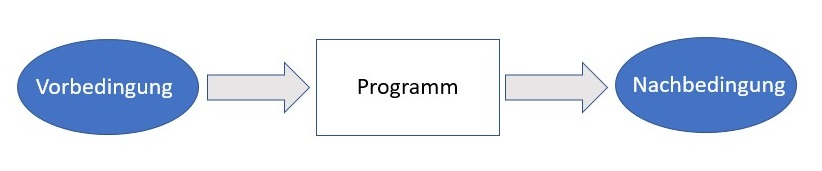
\includegraphics[width=\textwidth]{images/VorNachbedingungDijkstra}
	\caption{Logischer Aufbau eines Programms nach Dijkstra, eigene Darstellung}
	\label{img:VorNachbedingungDijkstra}
\end{figure}

Das einhalten von Vor- und Nachbedingungen ist in moderner Softwareentwicklung stets gefordert. Weil das anwenden von Beweisführungen und Schlussregeln auf Programmen heutzutage zu komplex sind und für den Menschen in komplexen Softwarearchitekturen nur noch schwer nachzuvollziehen sind, wird explizit Code entwickelt, der den entwickelten Code testet. Das führt zur Unterscheidung zwischen Produktions- und Testcode. Der Testcode soll den Produktionscode auf korrektes Verhalten überprüfen.\cite{kirchner2017}

Nach der Auslieferung von Software können Fehler immer noch entdeckt werden, zum Beispiel durch den Kunden. Das bestätigt die These von Dijkstra:

\smallskip

\textbf{\glqq Durch Testen kann man stets nur die Anwesenheit, nie aber die Abwesenheit von Fehlern beweisen.\grqq} (vgl. Dijkstra E. W. - The Humble Programmer, ACM Turing Lecture 1972)

\smallskip

Diese These bestätigt Witte F. in \cite{witte2019testmanagement}. Testaktivitäten schlagen fehl und erzeugen Fehler. Nach \cite{witte2019testmanagement} ist das Risiko, dass noch unentdeckte Fehler im Testobjekt vorhanden sind geringer, je höher die Testabdeckung ist. Testen zeigt nicht, dass die Software fehlerfrei ist, selbst wenn keine Fehler nachgewiesen werden. Testen ist kein mathematischer Beweis. Softwaretests beziehen sich immer auf die Betrachtung von Stichproben, es werden nicht alle möglichen Eingabeparameter und deren Kombinationen mit allen möglichen Vorbedingungen getestet, sondern diejenigen, die am ehesten praxisrelevant sind. Der Testaufwand richtet sich dabei nach Priorität und Risiko. Der Aufwand ist dabei immer mit
dem Nutzen abzugleichen. 

\smallskip

Eine Software vollständig zu testen ist somit unmöglich. Ein Test dient zur Feststellung, ob ein Programm wie in der Spezifikation festgehalten
funktioniert und nichts anderes tut, aber nicht um alle möglichen Fehler ausschließen zu können.

\smallskip

Tests eines komplexen Software-Systems lassen sich in verschiedene Testarten einordnen. Nicht jeder Test ist in jedem Entwicklungsstand möglich. Weil aber nicht jede Teststufe oder Testart zu jedem Zeitpunkt möglich ist, müssen die Testarten eindeutig voneinander abgegrenzt werden.

\subsubsection*{Testarten:}

\begin{figure}[h]
	\centering
	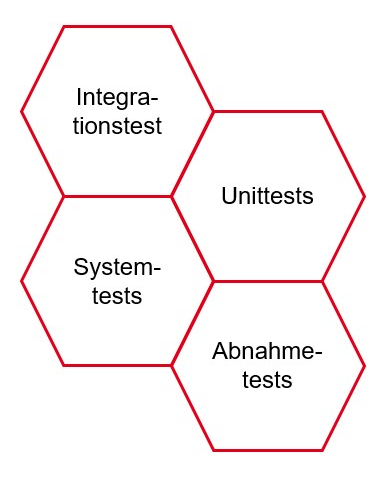
\includegraphics[width=6cm]{images/Testarten.png}
	\caption{Übersicht über Testarten, eigene Darstellung}
	\label{img:Testarten}
\end{figure}

Die häufigsten Testarten lassen sich in vier Bereiche aufteilen - Integrationstests, Unittests, Systemtests und Abnahmetests, siehe \autoref{img:Testarten}. \textbf{Integrationstests} sind abgestimmte Reihen von mehreren Tests, die dazu dienen, verschiedene voneinander abhängige Komponenten eines komplexen Systems im Zusammenspiel miteinander zu prüfen. Für den Integrationstest erstellt man nun Testszenarien, die das Zusammenwirken der beiden betroffenen Komponenten zeigen. Die Anzahl der Integrationsstufen richtet sich nach der Komplexität der Software. \textbf{Systemtests} werden durchgeführt, um die gesamte Software gegen die gesamten Anforderungen des Kunden zu testen. Das beinhaltet alle funktionalen Anforderungen und nicht funktionalen Anforderungen, wie zum Beispiel Qualität oder Bedienbarkeit. Weil Systemtests die gesamte Software testen, sind diese zum Zeitpunkt der Fertigstellung der Software durchzuführen. Idealerweise wird die Produktivumgebung des Kunden zuerst nachgestellt und die Software mit Live-Szenarien aus dem Produktivbetrieb getestet. Ein \textbf{Abnahmetest}, \textbf{Verfahrenstest}, \textbf{Akzeptanztest} oder auch \textbf{User Acceptance Test} ist ein Test der ausgelieferten Software durch den Kunden und/oder Auftraggeber. Der Test wird oft mit Kopien von echten Daten in der Produktionsumgebung des Kunden durchgeführt. Diese Testart hat nicht das Ziel Fehler zu entdecken, sondern das der Kunde Vertrauen in das Endprodukt gewinnt. Fehler sollten schon durch andere Testarten entdeckt worden und behoben sein. Zum Beispiel durch \textbf{Unittests}. Unittests eignen sich dafür, bei jedem Entwicklungsstand einzusetzen. Diese Art von Tests werden in der Softwareentwicklung durchgeführt, um kleine, funktionale Einzelteile (\textbf{Units}) zu testen. Ein \textbf{Unit} kann dabei ein kleiner Codeabschnitt sein oder eine Methode einer Klasse sein. Weil Algorithmen auf Modulebene meist nur eine begrenzte Komplexität aufweisen und über klar definierte Schnittstellen aktiviert werden, können sie mit relativ wenigen Testfällen ziemlich umfassend getestet werden.\cite{witte2019testmanagement}

\smallskip

Eine wichtige Anforderung an Tests ist, dass diese schnell und effizient ablaufen. Effizient, um nicht mehr als die notwendigen Ressourcen zu verbrauchen und schnell, um möglichst oft aufgerufen zu werden.\cite{hubertz2016softwaretests} Diese Anforderungen erfüllen vor allem Unittests, weshalb für die Entwicklung der Softwarefunktionalitäten des Projekts Unittests eingesetzt werden. Diese werden im nächsten Kapitel genauer erläutert. 

\subsection{Unittests}
\label{Unittests}

\chapter{Umsetzung und Implementierung}
\label{chap:Umsetzung}

\section{Aufbau und Entwurf der Architektur des Chatsystems}
\label{chap:Architektur}

Nach den Anforderungen (\autoref{Anforderungen}) und Zielen der Arbeit (\autoref{sec:Ziele}) soll ein \ac{IMS} auf Basis eines \ac{XMPP}-Chatsystems entworfen und programmiert werden. Anschließend soll das gleiche Chatsystem auf Basis des Frameworks Apache Kafka mit Kafka Streams implementiert und mit dem \ac{XMPP}-Chatsystem verglichen werden. Hierfür muss ein verteiltes System entworfen werden, das die Anforderungen abdeckt.

Der Autor Tanenbaum definiert ein verteiltes System wie folgt: \glqq Ein verteiltes System ist eine Ansammlung unabhängiger Computer, die den Benutzern wie ein einzelnes kohärentes System erscheinen.\grqq \footnote{\cite[S.19]{andrew2008verteilte}} Die Definition von Tanenbaum hat mehrere wichtige Aspekte. Der Erste besagt, dass ein verteiltes System aus Komponenten besteht, die autonom sind. Sie bieten einen Dienst an oder haben eine bestimmte Aufgabe und eine lokale Zeit. Ein zweiter Aspekt ist, dass die Benutzer glauben, sie hätten es mit einem einzigen System zu tun. Die Eigenschaft \glqq kohärenz\grqq aus der Definition besagt, dass die Komponenten in einer bestimmten Art und Weise zusammen arbeiten, um den Benutzer einen Dienst zu erbringen. Ein besonderes Merkmal ist, dass keinerlei Annahmen über die Art der Computer getroffen werden. Diese können heterogen sein. Tanenbaum \cite{andrew2008verteilte} ist der Ansicht, dass die Herausforderungen eines verteilten Systems sind, die einzelnen Teilsysteme zu synchronisieren und die Zusammenarbeit korrekt zu implementieren.

Hierzu stellt sich die Frage, welche Dienste für das Chatsystem benötigt und wie die Dienste auf Komponenten sinnvoll verteilt werden. Der erste Teil der Frage kann mit Hilfe der Anforderungen aus \autoref{Anforderungen} beantwortet werden. Folgende Auflistung beinhaltet wichtige Funktionalitäten die als Komponenten zusammengefasst sind:

\begin{itemize}
\item Client für Benutzer, um Chat-Funktionalitäten durchführen zu können
\item ejabberd als \ac{XMPP}-Server für das \ac{XMPP}-basierte Chatsystem
\item Apache Kafka mit Kafka Streams
\item Datenbank für Authentifizierung und Archivierung von Nachrichten
\end{itemize}

\newpage

Für die Beantwortung der Fragestellung, wie die Dienste auf Komponenten verteilt werden, bedarf es noch weiteren Untersuchungen. Theoretisch könnten alle Dienste bis auf den Chat-Client auf einer einzelnen Server-Instanz realisiert werden. Ein Vorteil ist, dass einzelne Dienste ohne Netzwerklatenzen miteinander kommunizieren können und Daten direkt austauschen können. Latenzen entstehen dann nur bei der Übertragung von Nachrichten vom Server zum Chat-Client und umgekehrt oder aufgrund der Bearbeitungszeit eines Dienstes. Dieser Architektur ist kritisch anzumerken, das die einzelnen Dienste um Ressourcen konkurrieren könnten und die Funktionsfähigkeit stark von der Qualität und der Leistung des Servers abhängig ist. Hinzu kommt, dass wenn der Server ausfällt oder beschädigt wird, jeder Dienst nicht mehr erreichbar ist. Das wäre entgegen den Vorteilen und Absichten von verteilten Systemen. Um die Architektur zu verbessern müssen die Eigenschaften und Ziele von verteilten Systemen berücksichtigt werden. Tanenbaum geht darauf detailliert in \cite{andrew2008verteilte} ein.

\subsubsection*{Eigenschaften von verteilten Systemen}

Eine Eigenschaft ist, dass die Unterschiede der Komponenten und die Art, wie sie untereinander kommunizieren, weitestgehend vor den Benutzern verborgen bleiben. Das bedeutet, dass wenn ein Benutzer eine Nachricht zu einem anderen Benutzer über das \ac{IMS} sendet, darf ein Benutzer nicht mitbekommen, wie viele und welche Instanzen mitwirken, um die Nachricht ihrem Empfänger zuzustellen. Eine weitere wichtige Eigenschaft ist, dass Benutzer konsistent mit dem verteilten System arbeiten können, egal wo und wann diese Zusammenarbeit stattfindet. Die Tatsache, dass ein Benutzer am \ac{IMS} angemeldet ist und Nachrichten versendet, darf keine Aktionen anderer Benutzer beeinflussen. Darüber hinaus sollte es leicht erweiterbar und skalierbar sein. Dieser Aspekt ist in dem vorher beschrieben Ansatz nicht gegeben. Es können nicht beliebig viele Dienste auf einem Server realisiert werden und auch die Ressourcen eines einzelnen Servers können nicht beliebig erweitert werden. Ein weiterer Punkt ist,dass Benutzer und Anwendungen nicht bemerken sollen, dass Teile ersetzt, repariert oder neue Teile hinzugefügt werden, um mehr Benutzer oder Anwendungen bedienen zu können.\cite{andrew2008verteilte}
Auf den Aspekt der Redundanz wird in dieser Arbeit nicht eingegangen. Das Ziel ist es nicht die Fehlertoleranz durch redundante Komponenten und Anwendungen zu gewährleisten, vielmehr soll ein Prototyp mit ausreichenden Funktionalitäten eines \ac{IMS} entwickelt werden und zwei verschiedene Implementierungsformen verglichen werden.



\pagebreak

\section{Ejabberd als moderner Chatserver}
\label{sec:ejabberd}

Ejabberd ist einer der bekanntesten \ac{XMPP}-Server auf der Welt und kann in vielerlei Hinsicht verwendet werden. Er ist lizenzfrei benutzbar und unterstützt das Betriebssystem Windows, Linux und Mac OS. Sowohl Großprojekte als auch kleine Instanzen machen sich die Eigenschaften von ejabberd zum Vorteil. Der Start von ejabberd ist dem Jahr 2002 zuzuordnen. Ejabberd ist eine Abkürzung und steht für \glqq Erlang Jabber Daemon\grqq. Wie die Definition zeigt bezieht sich ejabberd auf die Programmiersprache Erlang. Grund hierfür ist, dass die ejabberd Software in Erlang geschrieben ist. Seit dem Start wurde es von Grund auf für die Unternehmensbereitstellung entwickelt, vor allem mit dem Ziel robust zu sein. Aufgrund davon, dass der Fokus auf die Unternehmen lag, war es wichtig die Fehleranfälligkeit von ejabberd zu minimieren. Ein Vorteil der sich bis zum heutigen Zeitpunkt bewahrt hat. Außerdem kann ejabberd die Ressourcen mehrerer geclusterter Systeme nutzen. Des Weiteren besitzt ejabberd die Eigenschaft der Skalierbarkeit, indem die Kapazitäten mit wenig Aufwand erhöht werden kann. Während der Entstehungsphase war das \ac{XMPP}-Protokoll, welches in \autoref{sec:XMPP} beschrieben wird, noch unter dem Namen Jabber bekannt. Ejabberd kann verschieden benutzt werden. Im Fall der Studienarbeit wird die Community Edition von ejabberd benutzt, welche als open source zur Verfügung steht. Neben der Community Edition gibt es auch noch Möglichkeiten einer Business Edition, welches vor allem für die großen Unternehmen mit besserem Support und mehr Funktionen konzeptioniert ist. Die Architektur eines ejabberd-Services erweitert die Kernfunktionen von \ac{XMPP}, welches das Senden von Nachrichten ist, um Faktoren wie die Skalierbarkeit, Konfigurierbarkeit und Fehlertoleranz.

\bigskip

\textbf{Relevante Funktionen:}

\begin{itemize}
	\item Einzelchat
	\item Gruppenchat (auch als Multi-User-Chat (\ac{MUC}) bezeichnet)
	\item Offline Nachrichten 
	\item Web-Unterstützung
	\item Nachrichtenübermittlungsbestätigung
	\item Übermittlung des Online-Status
	\item Verschlüsselte Übertragung von Nachrichten
	\item Kontaktliste jedes Benutzers
\end{itemize}

Die Architektur von ejabberd ist modular. Das bedeutet, dass die Architektur an den Zweck eines Projektes angepasst werden kann.

\autoref{img:ArchitekturEjabberd} zeigt eine Übersicht über die Architektur und die Flexibilität von ejabberd \cite{ejabberdModulesDeployment}.

\begin{figure}[h]
	\centering
	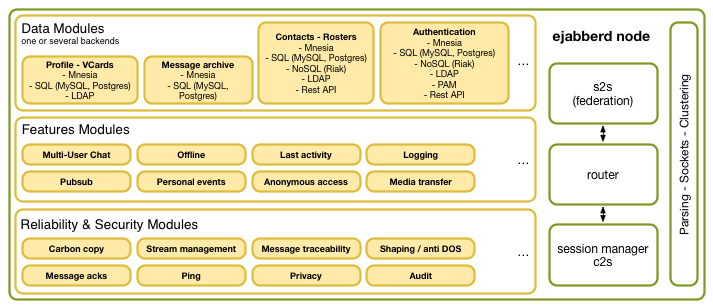
\includegraphics[width=\linewidth]{images/ejabberd_internals}
	\caption{Übersicht über die Architektur von ejabberd \cite{ejabberdModulesDeployment}}
	\label{img:ArchitekturEjabberd}
\end{figure}

Die interne Architektur von ejabberd setzt auf dem Router auf. Der Router leitet Anfragen an interne Dienste und Module weiter oder versendet Nachrichten. Neben der Kommunikation zwischen Clients und Server (c2s) unterstützt ejabberd die Kommunikation zu anderen \ac{XMPP}-Servern (s2s) und kann in bereits vorhandenen \ac{XMPP}-Domänen integriert werden. Die meisten anderen Elemente sind Plugins, die angepasst, erweitert oder ersetzt werden können, um eine benutzerdefinierte Lösung zu erstellen, die auf konkrete Anforderungen zugeschnitten ist. So lassen sich zum Beispiel Funktionen wie \ac{MUC} oder Logging benutzerdefiniert konfigurieren, siehe Feature Modules in \autoref{img:ArchitekturEjabberd}. Unerwünschte Module können deaktiviert werden. Eine wichtige Eigenschaft ist das Authentifizieren von Benutzern. Dafür kann ejabberd sowohl mit einer internen, als auch mit einer externen Datenbank zusammenarbeiten. Der Block Data Modules in \autoref{img:ArchitekturEjabberd} zeigt, dass ejabberd neben der Authentifizierung auch die Archivierung von Nachrichten (Message archive) oder die Verwaltung von Kontaktlisten (Contacts-Rosters) unterstützt. Aufgrund der genannten Eigenschaften und Funktionen von ejabberd, werden eine viele Anwendungsgebiete abgedeckt.\cite{ejabberdModulesDeployment, ejabberdDoc}

Während für kleine Projekte die interne Datenbank Mnesia ausreichend ist, wird in der Studienarbeit mit einer externen Datenbank gearbeitet. In den folgenden zwei Kapiteln wird erläutert, wie eine ejabberd-Instanz mit der Verwendung einer externen MySQL Datenbank installiert werden kann. Ferner wird beschrieben, wie die Standardkonfiguration so angepasst werden kann, dass der Server sicher und datenschutzfreundlich ist.

\pagebreak

\section{Implementierung des Chatservers ejabberd}
\label{sec:ChatserverEntwicklung}

Die Grundlagen von ejabberd wurden im \autoref{sec:ejabberd} erläutert. In diesem Abschnitt wird beschrieben, welche Schritte notwendig sind, um den Chatserver ejabberd zu installieren und gemäß den Anforderungen aus \autoref{Anforderungen} zu konfigurieren.

\section{Installation des Chatservers ejabberd}
\label{sec:InstallationEjabberd}

\subsubsection*{Hardware und Betriebssystem}

Die Mindestanforderungen an Hardware sind in der ejabberd Dokumentation in \cite{ejabberdDocGettingStarted} nicht beschrieben. Die Dokumentation enthält Richtwerte für die Anzahl an Cores und die Menge an Arbeitsspeicher (RAM). Das System unterstützt bei 16 GB RAM und vier Cores insgesamt 200-300 Benutzer und zehn Clients gleichzeitig. Der Betreiber des Systems muss die Richtwerte an die Skalierung seines Systems selbst anpassen. Weil das System nach den Anforderungen keine große Anzahl an Benutzern unterstützen muss, wird eine Installation mit den folgenden Hardwarespezifikationen auf einer virtuellen Maschine umgesetzt:

\begin{itemize}
\item CPU: 2 vCPU
\item Kapazität des Arbeitsspeichers (RAM): 4 GB
\item Kapazität des persistenten Speichers: 12 GB
\end{itemize}

Die ejabberd Software unterstützt nach \autoref{sec:ejabberd} das Betriebssystem Linux. Für die Installation wird ein Linux Ubuntu 18.04 (LTS) gewählt, weil das Betriebssystem lizenzfrei ist und kostenlos benutzt werden kann.

\subsubsection*{Installation}

Ejabberd wird als einzelne Instanz installiert. Es wird keine Installation als Cluster, das einen Verbund aus mehreren gleichwertigen ejabberd Instanzen definiert, benötigt.

Nach \autoref{sec:ejabberd} ist die interne Mnesia Datenbank des Chatservers zu klein, um einen voll umfänglichen Testbetrieb zu realisieren. Aus diesem Grund wird eine MySQL-Datenbank installiert und eine sichere Installation durchgeführt. Die sichere Installation entfernt vorinstallierte Datenbanken und stellt sicher, dass die Datenbank über keine andere IP-Adresse als über die localhost IP-Adresse erreichbar ist.

\bigskip

\begin{lstlisting}[language=bash, caption={Installation der Mysql-Datenbank}]
$ sudo apt install mysql-server
$ sudo mysql_secure_installation
\end{lstlisting}

Die Datenbankinstallation war erfolgreich, wenn der Verbindungsversuch mit dem root User des Betriebssystems erfolgreich verläuft. Der Befehl \textbf{sudo mysql -uroot} startet einen Verbindungsversuch.

Das relationale Datenbankschema das ejabberd benötigt, kann auf github heruntergeladen werden. Der erste Befehl lädt die SQL-Datei, in der das Datenbankschema definiert ist herunter. Der zweite Befehl erstellt in der Datenbank einen Benutzer \glqq ejabberd\grqq mit einem Passwort. Der Befehl in Zeile 3 schränkt die Zugriffsrechte des Benutzers auf die Datenbank \glqq ejabberd\grqq ein, die in Zeile 4 Listings erstellt wird. Der letzte Befehl spielt das Datenbankschema in die Datenbank \glqq ejabberd\grqq ein.

\bigskip

 \begin{lstlisting}[language=bash, caption={Installation der Mysql-Datenbank}]
$ sudo wget https://raw.githubusercontent.com/processone/ejabberd/master/sql/mysql.sql
$ echo "CREATE USER 'ejabberd'@'localhost' IDENTIFIED BY 'passwort' " | sudo mysql -uroot
$ echo "GRANT ALL ON ejabberd.* TO 'ejabberd'@'localhost' IDENTIFIED BY 'passwort';" | sudo mysql -uroot
$ echo "CREATE DATABASE ejabberd;" | sudo mysql -uejabberd -p
$ sudo mysql -D ejabberd -uejabberd -p < mysql.sql
\end{lstlisting}



Der folgende Befehl installiert den Chatserver ejabberd und den Datenbank Treiber für MySQL, sodass sich der Chatserver auf die MySQL-Datenbank verbinden kann. Der Treiber ist in der Programmiersprache Erlang programmiert.

\bigskip

\begin{lstlisting}[language=bash, caption={Installation von ejabberd und des MySQL Datenbanktreibers}]
$ sudo apt -y install ejabberd
$ sudo apt install erlang-p1-mysql
\end{lstlisting}

Weil der Chatserver den Transport der Daten verschlüsseln und die Authentizität gewährleisten soll, wird ein TLS-Zertifikat der Let' s Encrypt Zertifizierungsstelle (engl. \ac{CA}) erstellt und im Chatserver installiert. Zertifikate schützen vor nicht autorisierten Zugriffen und bestätigen die Authentizität. Zusätzlich bewahren sie die Integrität der übertragenen Daten.\cite{melzer2010web}

Let's Encrypt verwendet das ACME-Protokoll, um zu überprüfen, ob ein bestimmter Domainname vorhanden ist und um ein Zertifikat auszustellen. Für die Ausstellung von Let's Encrypt Zertifikaten wird eine ACME-Client-Software benötigt.\cite{letsencryptACME}

Der Chatserver ejabberd hat keine Client-Software vorinstalliert, die das ACME-Protokoll unterstützt. Aus diesem Grund muss der open-source ACME-Client \glqq acme.sh\grqq installiert werden. Dieser ist kompatibel mit der Linux-Bash. Der Standalone-Modus des ACME-Clients realisiert einen Webserver, der die Domain gegenüber der Let's Encrypt \ac{CA} validiert.\cite{acmeshOfficial}
Der ACME-Client und seine benötigten Pakete werden mit folgenden Befehlen installiert.

\bigskip

\begin{lstlisting}[language=bash, caption={Installation der ACME-Client-Software für die Domainvalidierung}]
$ apt install socat curl
$ wget -O - https://get.acme.sh | sh
\end{lstlisting}

Mit folgendem Befehl wird ein \ac{RSA}-Zertifikat angefordert, wobei die Zeichenkette \glqq xmpp-dhbw.spdns.org\grqq der Domainname ist. Der Befehl ist mit dem root Benutzer durchzuführen.

\bigskip

\begin{lstlisting}[language=bash, caption={Installation des Let's Encrpt Zertifikats durch den ACME-Client}]
$ bash /root/.acme.sh/acme.sh --issue -d xmpp-dhbw.spdns.org --keylength 4096 --standalone
\end{lstlisting}

Das Argument \glqq keylength 4096\grqq definiert die Länge des privaten Schlüssels in Bit. Laut den technischen Empfehlungen des \ac{BSI} ist ein Schlüssel mit 2000 bit Länge bis Ende des Jahres 2022 sicher. Danach sollen Schlüssel mit einer Mindestlänge von 3000 bit verwendet werden, die das \ac{BSI} bis Ende 2023 als sicher einstuft.\cite{empfehlungBSI}

Nach den Anforderungen aus \autoref{Anforderungen}, wird zur Sicherheit ein privater Schlüssel mit 4096 bit Länge konfiguriert. Der Ablauf einer Verschlüsselung mit Hilfe des \ac{RSA}-Verfahrens ist in [Kapitelnummer einfügen] beschrieben.

Das Zertifikat und die Schlüssel befinden sich nach ihrer Beantragung im Ordner \texttt{/root/.acme.sh/xmpp-dhbw.spdns.org}. Diese werden im ejabberd-Server in der Konfiguration eingebunden. Dazu wird ein Unterverzeichnis im Installationspfad von ejabberd erstellt (Befehl 1) und das Zertifikat und der private Schlüssel in den Unterordner kopiert (Befehle 2-3). Der Unterordner kann in der Konfiguration von ejabberd angegeben werden.
Die letzten drei Befehle schränken die Berechtigungen ein. Sie machen den Ordner selbst und die Zertifikatsdateien zum Eigentum vom ejabberd Benutzer. Der \texttt{chmod}-Befehl definiert mit 600 als Argument, das die Datei nur vom ejabberd Benutzer gelesen und beschrieben werden dürfen. Alle anderen Benutzer, die auf dem System existieren werden davon ausgeschlossen.

Die Befehle sind weiterhin mit dem root Benutzer durchzuführen.

\bigskip

\begin{lstlisting}[language=bash, caption={Kopieren der Zertifikate in ein Unterverzeichnis und Einschränkung der Rechte},label={lst:ejabberdCerts}]
$ mkdir /etc/ejabberd/certs
$ cp /root/.acme.sh/xmpp-dhbw.spdns.org/fullchain.cer /etc/ejabberd/certs/fullchain.pem
$ cp /root/.acme.sh/xmpp-dhbw.spdns.org/xmpp-dhbw.spdns.org.key /etc/ejabberd/certs/
$ chown ejabberd:ejabberd /etc/ejabberd/certs/
$ chown ejabberd:ejabberd /etc/ejabberd/certs/*
$ chmod 600 /etc/ejabberd/certs/*
\end{lstlisting}

Für \ac{PFS} wird eine Datei erzeugt, die Diffie-Hellman (DH) Parameter enthält. Die DH-Parameter bestehen aus zwei Zahlen p (eine sehr große Primzahl) und g (Generatorwert, in openSSL immer 2). Die DH-Parameter werden für den Schlüsselaustausch zwischen Client und ejabberd-Server verwendet, um zu gewährleisten, dass bei jeder Verbindung im Sinne der \ac{PFS} ein neuer Sitzungsschlüssel erzeugt wird und nicht über einen unsicheren Kommunikationskanal ausgetauscht werden muss. Durch das DH-Verfahren können sich beide Kommunikationspartner auf einen geheimen Sitzungsschlüssel einigen ohne ihn übertragen zu müssen. Für die Berechnung des Schlüssels werden nur die DH-Parameter aus der Datei übertragen. Nach der Sitzung wird der erzeugte Schlüssel gelöscht. Durch das Verfahren wird verhindert, dass der Sitzungsschlüssel rekonstruiert werden kann. Eine Datei mit DH-Parameter zu erzeugen, benötigt viele CPU-Ressourcen und nimmt einige Zeit in Anspruch.\cite{perfectForwardSecrecy}

Der folgende Befehl erzeugt DH-Parameter mit einer Länge von 4096 bit.

\bigskip

\begin{lstlisting}[language=bash, caption={Erzeugen von Diffie-Hellman-Parametern für den ejabberd-Server},label={lst:DHParameters}]
$ openssl dhparam -out /etc/ejabberd/dh4096.pem 4096
\end{lstlisting}

Nachdem alle zuvor erläuterten Vorbereitungsschritte durchgeführt sind, kann der ejabberd-Server gestartet und ein automatisches Starten des Dienstes beim Bootvorgang aktiviert werden:

\bigskip

\begin{lstlisting}[language=bash, caption={Starten der ejabberd-Instanz}]
$ sudo systemctl start ejabberd #start ejabberd service
$ sudo systemctl enable ejabberd #auto start on boot
$ sudo systemctl status ejabberd
\end{lstlisting}

Liefert die Statusabfrage (Befehl 3) keine Fehler, muss im nächsten Schritt ein Benutzer angelegt werden, der die nötigen Rechte besitzt, sich in das webbasierte Administrationsportal einzuloggen. Im Auslieferungszustand ist in der \ac{ACL} des ejabberd-Servers der Zugriff für die Administration auf den Benutzer \texttt{admin} beschränkt.\cite{ejabberdMGMT}

Alle anders genannten Benutzer können sich mit ihrem Passwort im Administrationsportal einloggen, sie können aber keine Konfigurationen lesen oder verändern. Dieses Verhalten wurde durch einen Selbstversuch festgestellt. Über das in erlang programmierte Skript kann ejabberd verwaltet werden. Der Benutzer \textbf{admin} wird mit folgendem Befehl angelegt:\cite{ejabberdMGMT}

\bigskip

\begin{lstlisting}[language=bash, caption={Anlegen eines Benutzers für die Verwaltung von ejabberd},label={lst:AddAdminUserEjabberd}]
$ sudo ejabberdctl register admin ejabberd-server passwort
\end{lstlisting}

Das Argument \texttt{register} ermöglicht das Anlegen des Benutzers. Das Argument \texttt{ejabberd-server} definiert die Domain innerhalb derer der Benutzer gültig ist. Es dürfen mehrere Domains auf dem Server registriert werden. Im Auslieferungszustand ist eine Domain \texttt{localhost} konfiguriert und das Administrationsportal ist unter \texttt{http://localhost:5280/admin} erreichbar. Damit das Administrationsportal mit dem Browser über die oben genannte Domain \texttt{http://xmpp-dhbw.spdns.org/admin} erreichbar ist und sich mit dem erstellten Benutzer innerhalb der Domain \texttt{ejabberd-server} eingeloggt werden kann, muss die Konfigurationsdatei angepasst werden.\cite{ejabberdMGMT}

Nach \cite{ejabberdDoc} ändert ejabberd die Konfigurationsdatei nicht, wenn ein Administrator Änderungen über das Administrationsportal durchführt. Es empfiehlt sich daher, die Administrationsoberfläche für die Benutzerverwaltung zu benutzen und die Konfiguration innerhalb der Datei anzupassen.

Die Konfiguration von ejabberd über seine Konfigurationsdatei ist im nächsten Kapitel beschrieben.


\section{Konfiguration von ejabberd}
\label{sec:Konfiguration}

Dieses Kapitel stellt eine Zusammenfassung wichtiger Konfigurationsschritte dar, die gemäß den Anforderungen aus \autoref{Anforderungen} durchgeführt wurden.

Ejabberd bietet zwei Konfigurationsdateien, die sich im Format unterscheiden. Mit beiden Dateien können dieselben Konfigurationen vorgenommen werden. Es empfiehlt sich, sich für ein Format zu entscheiden, um Inkonsistenzen oder Konfigurationsfehler zu vermeiden.

\autoref{img:YAMLconfig} zeigt die Konfiguration in der Formatierung \ac{YAML} und \autoref{img:ErlangConfig} in der Formatierung Erlang auch Legacy Configuration gennant. Nach dem offiziellen ejabberd Configuration Guide \cite{ejabberdDoc} ist die im Format Erlang existierende Datei \texttt{ejabberd.cfg} veraltet und Administratoren sollten diese in das Format \ac{YAML} umwandeln. Bei Neuinstallationen sollen Konfigurationen direkt in der Datei \texttt{ejabberd.yml} vorgenommen werden. Diese ist im Format \ac{YAML} geschrieben.

\begin{figure}
\centering
\begin{minipage}{.5\textwidth}
  \centering
  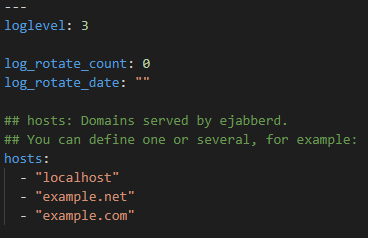
\includegraphics[width=.8\linewidth]{images/exampleYAMLConfig}
  \caption{Formatierung: \texttt{YAML}}
  \label{img:YAMLconfig}
\end{minipage}%
\begin{minipage}{.5\textwidth}
  \centering
  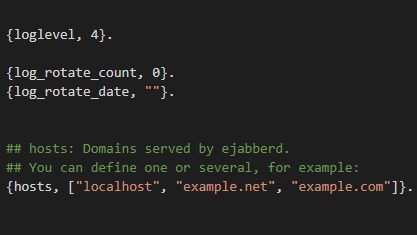
\includegraphics[width=.9\linewidth]{images/ejabberdErlangConfig}
  \caption{Formatierung: \texttt{Erlang}}
  \label{img:ErlangConfig}
\end{minipage}
\end{figure}

Eine genaue Beschreibung der Syntax und dem Aufbau ist in \cite{specificationYAML} vorhanden. \ac{YAML} ist eine vereinfachte Auszeichnungssprache (engl. markup language). Das Ziel des Designs \ac{YAML} ist die Annahme, dass sich jede beliebige Datenstruktur mit assoziativen Listen, Listen (Arrays) und Einzelwerten (Skalaren) darstellen lässt. In \autoref{img:YAMLconfig} beginnt ein in \ac{YAML} formatierter Abschnitt mit drei Bindestrichen. Danach ist beispielhaft ein Skalar \texttt{loglevel} aufgeführt, das wieder auf ein Skalar \texttt{3} abbildet. Diese Syntax entspricht dem Key-Value-Prinzip (Schlüssel-Wert-Prinzip). Die Skalare links vom Doppelpunkt sind Variablen, die auch innerhalb der \ac{YAML}-Datei mit \glqq \texttt{\{ variable \}}\grqq referenziert werden können. Werden mehrere Key-Value-Paare Zeile für Zeile aufgelistet, stellt diese Auflistung eine assoziative Liste dar. Das Skalar \texttt{host} ist eine Liste, die mehrere Elemente enthält. Deren Elemente beginnen mit einem Bindestrich. Eine Verschachtelung von Ausdrücken ist durch Einrücken von Ausdrücken möglich. \ac{YAML} erlaubt keine Verwendung von Tabulatoren. Eine Einrückung wird durch eine bestimmte Anzahl an Leerzeichen erzielt. Zeilen mit \texttt{\#} am Anfang sind Kommentare. Durch dieses Konzept ist \ac{YAML} wesentlich leichter von Menschen zu lesen und zu schreiben, außerdem vereinfacht es die Weiterverarbeitung der Daten, da die meisten Sprachen, wie C++, Python oder Java solche Konstrukte bereits integriert haben.

Für das Projekt wird die Konfiguration von ejabberd entsprechend den Empfehlungen aus dem Configuration Guide \cite{ejabberdDoc} in der Auszeichnungssprache \ac{YAML} durchgeführt.

\subsubsection*{Aspekte der Konfiguration}

\begin{itemize}
\item Es werden ausschließlich Clients, die die Kommunikation über das Protokoll \ac{XMPP} unterstützt, wie zum Beispiel Gajim oder Morzilla Thunderbird.

\item Neue Accounts von Benutzern können über In-Band-Registration, das bedeutet, direkt über den \ac{XMPP}-Client eröffnet werden.

\item Es ist grundsätzlich jedem Benutzer gestattet einen Account anzulegen.

\item Aus- und eingehende Kommunikation ist über \ac{TLS} verschlüsselt. Kann der verschlüsselte Kanal nicht aufgebaut werden, zum Beispiel weil der Client die vom Server angebotenen Verschlüsselungsalgorithmen nicht unterstützt, wird die Verbindung abgebrochen.

\item Die Sammlung kryptographischer Verfahren zur Verschlüsselung von Transportdaten (engl. Cipher-Suites) ist im Sinne der Anforderungen aus \autoref{Anforderungen} und des Datenschutzes aus \autoref{chap:Datenschutz} sehr strikt.

\item Die Konfiguration ist nicht für ein Cluster-System oder für die Kopplung von mehreren \ac{XMPP}-Servern vorgesehen.

\end{itemize}

\autoref{tab:PortsEjabberd} zeigt eine Übersicht über alle Standardports und ihrer zugehörigen Dienste.

\begin{table}[h]
\centering
\caption{Übersicht über Ports von ejabberd und deren Dienste}
\begin{tabular}{|l|p{.9\textwidth}|}
\hline
\textbf{Port} & \textbf{Beschreibung} \\
\hline
\textbf{5222} & Clients, die sich über \ac{XMPP} mit dem Server verbinden und kommunizieren wollen, benutzen diesen Port. \\
\hline
\textbf{5223} & \ac{XMPP}-Clients, die sich direkt über \ac{TLS} mit dem Server verbinden wollen, benutzen diesen Port. \\
\hline
\textbf{5269} & Server, die sich mit dem ejabberd-Server verbinden wollen, nutzen diesen Port. \\
\hline
\textbf{5270} & Server, die sich direkt über \ac{TLS} mit dem ejabberd-Server verbinden wollen, benutzen diesen Port.  \\
\hline
\textbf{5280} & Der Zugriff auf das webbasierte Administrationsportal ist unter diesem Port für autorisierte Benutzer möglich. \\
\hline
\end{tabular}
\label{tab:PortsEjabberd}
\end{table}
%TODO xmpp compliance check am ende der config durchführen und beschreiben
Die im Folgenden beschriebenen Konfigurationen weichen von der Standardkonfiguration im Auslieferungszustand ab und dienen dem Zweck einer datenschutzfreundlichen und sicheren Konfiguration.

\subsubsection*{Änderung der Datenbank}

Wie in \autoref{sec:Datenbank} beschrieben, ist die interne Mnesia Datenbank nicht für die Verwendung in Produktivumgebungen geeignet und hat nur eine Speicherkapazität von maximal 2 GB. Aus diesem Grund wird die Konfigurationsdatei so angepasst, dass alle Daten in der in \autoref{sec:InstallationEjabberd} installierten MySQL Datenbank gespeichert werden. \autoref{lst:EjabberdDBEinstellung} zeigt die Einstellungen für die Datenbank, die ejabberd verwenden soll.

\bigskip

\begin{lstlisting}[language=yaml, caption={Anpassung der Einstellungen für die Datenbank},label={lst:EjabberdDBEinstellung}]
auth_method: sql
default_db: sql
sql_type: mysql
sql_server: "127.0.0.1"
sql_database: "ejabberd"
sql_username: "ejabberd"
sql_password: "passwort"
sql_port: 3306
\end{lstlisting}

Als Standarddatenbank wird mysql festgelegt. Die Datenbank läuft auf demselben Server wie ejabberd und der Datenbankname ist der des installierten SQL-Schemas, siehe \autoref{sec:InstallationEjabberd}. Hier ist kritisch anzumerken, dass die Zugangsdaten der Datenbank direkt sichtbar in der Konfigurationsdatei hinterlegt sind. Im offiziellen Administration Guide \cite{plainTextConfigSecurity} ist empfohlen, dass nur autorisierte Benutzer ein Lese- und Schreibrecht auf die Konfigurationsdatei bekommen sollen. Dabei stellt sich allerdings die Frage, inwiefern sich das System trotz der eingeschränkten Rechte von Angreifern kompromittieren lässt. Erlangt ein Angreifer die Benutzerdaten eines autorisierten Benutzers hat er uneingeschränkten Zugriff auf sensible Informationen. Wünschenswert wäre eine bessere Möglichkeit, sensible Informationen abzusichern.

\subsubsection*{Konfiguration des Logging}

Das Log-Level bestimmt den Grad der Ausführlichkeit von Einträgen in eine Protokolldatei. Es beeinflusst die Anzahl und den Detailgrad der Informationen, die die Software von ejabberd während dem Betrieb aufzeichnet.\cite{ejabberdDoc}

Verfügbare Log-Level nach \cite{ejabberdDoc}:

\begin{description}
\item[0] Der Server protokolliert alle Aktivitäten, zum Beispiel IP-Adressen von Clients, weitere Informationen zur Verbindung, Fehler und Warnungen.
\item[1] Critical: nur kritische, interne Fehler werden protokolliert. Warnungen und andere Informationen über Benutzer und Verbindungen sind ausgeschlossen.
\item[2] Error: Jeder Fehler wird protokolliert. Andere Informationen über Benutzer oder Verbindungen werden nicht gespeichert.
\item[3] Warning: Alle Warnungen und Fehler werden protokolliert, Verbindungsdetails und Informationen über den Benutzer nicht.
\item[4] Info: Verbindungsdetails und Informationen über den Benutzer werden protokolliert, zusätzlich Warnungen und Fehler jeglicher Art.
\item[5] Debug: Alle Informationen, Fehler und Warnungen werden protokolliert. Detaillierte Informationen über einzelne Module für die Fehlersuche werden erhoben.
\end{description}

Das Log-Level wird auf den Wert \texttt{3} (Warning) gesetzt. Dadurch wird verhindert, das Anmeldevorgänge von Clients oder das Versenden von Nachrichten erfasst wird. Nur Warnungen oder Fehler werden protokolliert.\cite{ejabberdDoc}

\bigskip

\begin{lstlisting}[language=yaml, caption={Einstellung für das Log-Level von ejabberd}]
loglevel: 3
hide_sensitive_log_data: true
\end{lstlisting}

Weil die Option \texttt{hide\_sensitive\_log\_data} aktiviert ist, werden keine IP-Adressen und sensitive Daten protokolliert. Diese Einstellung erhöht die Privatsphäre der Benutzer.\cite{ejabberdDoc}

\subsubsection*{Konfiguration des Host}

Die Liste \texttt{hosts} in \autoref{lst:configHosts} auf Seite \pageref{lst:configHosts} definiert die Domains, deren Benutzer zugeordnet werden können. Eine ejabberd-Instanz kann mehrere Domains verwalten und bedienen. Das Listing zeigt die Konfiguration von ejabberd mit der Domain \texttt{ejabberd-server}. Es ist zulässig, der Liste weitere Domains hinzuzufügen. Für das Projekt wird jedoch nur eine Domain benötigt.

\bigskip

\begin{lstlisting}[language=yaml, caption={Konfiguration der Domains},label={lst:configHosts}]
hosts:
  - "ejabberd-server"
\end{lstlisting}

Die Domain ist gleichzeitig die \ac{XMPP}-Domain mit der Benutzer adressiert werden können. Der Name des Benutzers muss innerhalb der Domain eindeutig sein und mit der vollständigen Domain konkateniert werden, zum Beispiel: \texttt{testuser@ejabberd-server}. Andernfalls ist die Adressierung zum Beispiel für das Versenden und dem Empfang einer Nachricht inkorrekt.
%TODO eventuell Grafik mit Senderdomain und Empfängerdomain und dazwischen Server

\subsubsection*{Konfiguration der Zertifikate}

Wie Zertifikate für die Verschlüsselung der Transportdaten beantragt werden können, ist in \autoref{sec:ChatserverEntwicklung} beschrieben. Nach \autoref{lst:ejabberdCerts} befindet sich das Zertifikat und die Datei, die den privaten Schlüssel enthält, im Ornder \texttt{/etc/ejabberd/certs}. Der Ort der Zertifikate muss in der Konfigurationsdatei angegeben werden, sodass ejabberd und ein Client einen verschlüsselten Kanal aufbauen können.

\bigskip

\begin{lstlisting}[language=yaml, caption={Konfiguration der Zertifikate}]
certfiles:
  - "/etc/ejabberd/certs/fullchain.pem"
  - "/etc/ejabberd/certs/xmpp-dhbw.spdns.org.key"
\end{lstlisting}

In der Liste \texttt{certfiles} sind das \ac{RSA}-Zertifikat und die Datei, die den privaten Schlüssel für das Entschlüsseln empfangener Daten beim Aushandeln des Session-Keys beinhaltet, angegeben. Nun kann ein Client das Zertifikat anfordern, mit Hilfe des öffentlichen Schlüssels die Authentizität des Servers überprüfen und den erzeugten Session-Key verschlüsselt übertragen. Der Server entschlüsselt den Session-Key mit seinem privaten Schlüssel aus der \texttt{.key}-Datei.

\subsubsection*{Konfiguration der \ac{TLS}-Parameter}

Der Betreiber von verschlüsselten Diensten muss zwischen Abwärtskompatibilität und Sicherheit abwägen. Beide Aspekte beeinflussen sich gegenseitig. Der Betreiber muss festlegen, ob die Anforderungen an das System ihn dazu zwingen, die Sicherheit des Systems zu reduzieren, sodass Clients, die nur schwächere Verschlüsselungsalgorithmen beherrschen, ebenfalls unterstützt werden. Ist das nicht der Fall, können solche Clients ausgeschlossen und nur noch als sicher eingestufte Algorithmen erlaubt werden, um die Gefährdung der Benutzer zu minimieren.\cite{melzer2010web}

Ein Betreiber eines IT-Service kann sich im offiziellen Wiki des Morzilla Project bei der Wahl der \ac{TLS}-Parameter Unterstützung einholen. Unter \url{https://wiki.mozilla.org/Security/Server_Side_TLS} sind empfohlene Konfigurationen aufgelistet, die nach Kompatibilitätsgrad gruppiert sind.
Die Cipher-Suites, die im Auslieferungszustand vorhanden sind, sind für eine optimale Abwärtskompatibilität zu Clients und zu anderen \ac{XMPP}-Servern ausgelegt und sind nicht sehr strikt. Die Anforderungen aus \autoref{Anforderungen} beinhaltet eine datenschutzfreundliche und sichere Konfiguration. Aus diesem Grund werden nur aktuelle Verschlüsselungsalgorithmen erlaubt und ältere, bereits von der \ac{BSI} als unsicher eingestufte Cipher-Suites werden ausgeschlossen (Stand April 2020).

\bigskip

\begin{lstlisting}[language=yaml, caption={Konfiguration der \ac{TLS} Cipher Suites}, label={lst:ejabberdCipherSuites}]
define_macro:
  'TLS_CIPHERS': "ECDHE-ECDSA-AES256-GCM-SHA384:ECDHE-RSA-AES256-GCM-SHA384:ECDHE-ECDSA-CHACHA20-POLY1305:ECDHE-RSA-CHACHA20-POLY1305:ECDHE-ECDSA-AES128-GCM-SHA256:ECDHE-RSA-AES128-GCM-SHA256:ECDHE-ECDSA-AES256-SHA384:ECDHE-RSA-AES256-SHA384:ECDHE-ECDSA-AES128-SHA256:ECDHE-RSA-AES128-SHA256"
  'TLS_OPTIONS':
    - "no_sslv3"
    - "no_tlsv1"
    - "no_tlsv1_1"
    - "cipher_server_preference"
    - "no_compression"
  'DH_FILE': "/etc/ejabberd/dh4096.pem"

c2s_ciphers: 'TLS_CIPHERS'
s2s_ciphers: 'TLS_CIPHERS'
c2s_protocol_options: 'TLS_OPTIONS'
s2s_protocol_options: 'TLS_OPTIONS'
c2s_dhfile: 'DH_FILE'
s2s_dhfile: 'DH_FILE'
\end{lstlisting}

Um benutzerdefinierte Cipher-Suites für den \ac{TLS}-Verbindungsaufbau zu konfigurieren, werden wie in \autoref{lst:ejabberdCipherSuites} dargestellt, Makros definiert. Das Schlüsselwort \texttt{define\_macro} leitet die Definition von Makros ein. Ein Makro beginnt und endet mit einem Hochkomma, dazwischen wird ein Bezeichner definiert. Dem Makro ist ein Wert zugewiesen. In Zeile 2 des Listings ist das Makro \texttt{TLS\_CIPHERS} definiert, das auf einen Zeichensatz abbildet, der die strikteren Cipher-Suites enthält. So werden nur als sicher eingestufte Verschlüsselungsalgorithmen wie zum Beispiel \ac{AES} mit 128 Bit oder 256 Bit unterstützt. Bereits als unsicher eingestufte Verschlüsselungen wie \ac{DES} werden damit deaktiviert. Das Makro \texttt{TLS\_OPTIONS} definiert die \ac{SSL}-Versionen. Durch den Parameter \texttt{no\_tlsv1\_1} in der Liste, wird ausgeschlossen, dass sich ein Client über ältere \ac{SSL}-Protokollversionen als \ac{TLS}-Version 1.2 mit dem Server verbinden kann. Nur \ac{TLS}-Version 1.2 oder höher werden vom Server unterstützt. Können Server und Client keine Verschlüsselungsalgorithmen oder \ac{TLS}-Versionen vereinbaren, die sie beide unterstützen, lehnt der Server die Verbindung ab. In Zeile 9 ist das Makro \texttt{DH\_FILE} definiert, das auf den absoluten Pfad zur der Datei abbildet, die die erzeugten Diffie-Hellman-Parameter (\autoref{lst:DHParameters}) enthält. In den letzten sechs Zeilen ist aufgezeigt, wie die Makros innerhalb der Konfigurationsdatei referenziert und genutzt werden können. Die benutzerdefinierten Cipher-Suites werden für Verbindungen von Client zu Server (\texttt{c2s\_ciphers}) und Server zu Server (\texttt{s2s\_ciphers} konfiguriert. Zusätzlich werden die benutzerdefinierten Protokollversionen und die Diffie-Hellman-Parameter dem ejabberd-Server zugewiesen. Die Verbindung ist somit mit aktuellen Algorithmen verschlüsselt und Perfect Forward Secrecy (\ac{PFS}) durch die Diffie-Hellman-Parameter vorhanden.

\subsubsection*{Konfiguration der Dienste}

Für die Kommunikation mit Clients oder Servern müssen die Standard-Ports aus \autoref{tab:PortsEjabberd} konfiguriert werden. \autoref{lst:ejabberdPortsConfig} zeigt die Standardkonfiguration, die so ergänzt wurde, dass die Änderungen die Sicherheit des Gesamtsystems positiv beeinflussen.

\bigskip

\begin{lstlisting}[language=yaml, caption={Konfiguration der Ports}, label={lst:ejabberdPortsConfig}]
listen:
  -
    port: 5222
    ip: "::"
    module: ejabberd_c2s
    starttls_required: true
    max_stanza_size: 65536
    shaper: c2s_shaper
    access: c2s
  -
    port: 5223
    ip: "::"
    module: ejabberd_c2s
    tls: true
    max_stanza_size: 65536
    shaper: c2s_shaper
    access: c2s
  -
    port: 5269
    ip: "::"
    module: ejabberd_s2s_in
  -
    port: 5270
    ip: "::"
    module: ejabberd_s2s_in
    tls: true
  -
    port: 5280
    ip: "::"
    module: ejabberd_http
    web_admin: true
\end{lstlisting}

\ac{XMPP}-Clients verbinden sich über Port 5222 mit dem Chatserver. Das wird dadurch festgelegt, dass diesem Port das Modul \texttt{ejabberd\_c2s} zugewiesen wird. Der Wert \glqq ::\grqq für die IP-Adresse bewirkt, dass der Server auf jeder seiner Netzwerkkarten und IP-Adressen Anfragen akzeptiert. Die Standardkonfiguration wird so ergänzt, dass \texttt{STARTTLS} bei jedem Verbindungsversuch vorausgesetzt wird. Die Option \texttt{max\_stanza\_size} bestimmt die maximale Anzahl an Bytes, die ein \ac{XMPP}-Stanza haben darf. Ist die Anzahl an Bytes über den konfigurierten Wert (65536), wird die Verbindung abgebrochen. In der Standardkonfiguration ist dieser Wert auf \texttt{infinity} gesetzt. Ein Angreifer kann den Server überlasten, wenn er eine hohe Anzahl an sehr großen \ac{XMPP}-Stanzas pro Session sendet. Diese Art des Angriffs bezeichnet man als \ac{DOS}. Die Begrenzung des Wertes vermindert die Wahrscheinlichkeit für den Erfolg eines solchen Angriffs.\cite{XMPPDOS}

Der Port 5223 ergänzt die Standardkonfiguration, sodass sich ein Client direkt via \ac{TLS} verbinden kann. Das bewirkt die Einstellung \texttt{tls: true}, die \texttt{starttls\_required: true} ersetzt.

Für die Verbindung von \ac{XMPP}-Servern zur ejabberd-Instanz ist der Standardport 5269 zuständig. Die Einstellung \texttt{ejabberd\_s2s\_in} bindet diesen Dienst an den Port. Für alle Verbindungen, die durch andere Server initiiert werden, ist \texttt{STARTTLS} notwendig. Das ist in der Standardkonfiguration in einer globalen Einstellung bereits festgelegt. Die globale Einstellung innerhalb der Konfigurationsdatei ist in diesem Listing nicht sichtbar.

Der Port 5270 ergänzt ebenfalls die Standardkonfiguration und dient dazu, dass Server sich direkt via \ac{TLS} mit ejabberd verbinden können.

Der Port 5280 implementiert das Modul \texttt{ejabberd\_http}. Durch die Einstellung \texttt{web\_admin: true} ist das Administrationsportal unter diesem Port verfügbar. Der Administrator dieses Projekts kann sich zum Beispiel unter dieser \ac{URI} in das Webportal einloggen: \texttt{https://xmpp-dhbw.spdns.org:5280/admin}.


\subsubsection*{Konfiguration der Zugriffskontrolle}

Ein Client authentifiziert sich gegenüber dem ejabberd-Server mittels \ac{SASL}. Nach \cite{SASLDescription} ist \ac{SASL} ein Framework, das von verschiedenen Protokollen im Internet für die Authentifizierung verwendet wird. Mittels \ac{SASL} handeln Client und Server standardisiert Authentifizierungsmethoden aus, die von der Applikation transparent genutzt werden.  Der Betreiber eines ejabberd-Servers sollte für eine sichere Konfiguration veraltete Authentifizierungsmethoden ausschließen.  

\bigskip

\begin{lstlisting}[language=yaml, caption={Ausschluss unsicherer Authentifizierungsmethoden}]
disable_sasl_mechanisms:
  - "digest-md5"
  - "x-oauth2"
\end{lstlisting}

Authentifizierungsmethoden die ausgeschlossen werden sollen, werden in die Liste \texttt{disable\_sasl\_mechanisms} eingetragen. Nach \ac{RFC} 6331 ist \texttt{digest-md5} veraltet und unsicher. Er benutzt intern einen \ac{MD5}, den ein Angreifer leicht ermitteln kann und ist empfindlich gegenüber Man-In-The-Middle-Angriffe.\cite{DigestMD5Vulnerabilty}

Auch \texttt{x-oauth2} hat mehrere Sicherheitslücken. Die Methode ist empfindlich gegenüber \ac{DOS}-Angriffe. Nach \cite{xOAuthVulnerabilty} kann ein nicht authentifizierter Angreifer, den Server überlasten.

In \autoref{lst:AddAdminUserEjabberd} auf Seite \pageref{lst:AddAdminUserEjabberd} ist beschrieben, wie ein Benutzer mit administrativen Rechten auf dem Server angelegt werden kann. In der Standardkonfiguration ist der Benutzer \glqq admin\grqq berechtigt auf das Administrationsportal mit der Domain \texttt{localhost} zuzugreifen. Damit der Benutzer berechtigt ist, auf die für das Projekt erstellte Domain \texttt{ejabberd-server} zuzugreifen, muss die \ac{ACL} angepasst werden. Hierfür trägt ändert man im Abschnitt \texttt{acl} der Konfigurationsdatei die Domain, auf die der Benutzer \glqq admin\grqq verweist. Das Ergebnis der Änderung ist in \autoref{lst:aclChangeAdmin} dargestellt.

\bigskip

\begin{lstlisting}[language=yaml, caption={Anpassung der Access Control List (ACL) für den administrativen Zugriff},label={lst:aclChangeAdmin}]
acl:
  admin:
     user:
       - "admin": "ejabberd-server"
\end{lstlisting}


Nach all den durchgeführten Änderungen muss der Server mit dem Kommando \texttt{sudo systemctl restart ejabberd} neu gestartet werden.

\subsubsection*{Überblick über das Administrationsportal}

Der Administrator kann sich mit Benutzername und Passwort in das Webportal einloggen. \autoref{img:AdminPortalEjabberdOverview} zeigt im linken Bild das Webportal nach einem Login.

\begin{figure}[h]
\centering
\begin{minipage}{.5\textwidth}
  \centering
  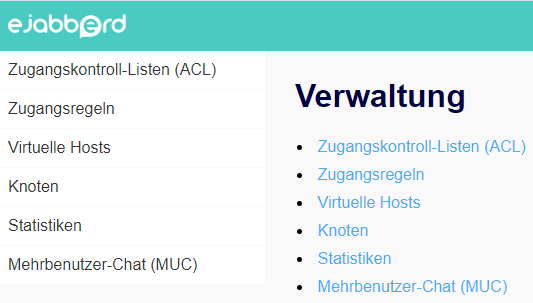
\includegraphics[width=.9\linewidth]{images/AdminPortalEjabberdOverview}
\end{minipage}%
\begin{minipage}{.5\textwidth}
  \centering
  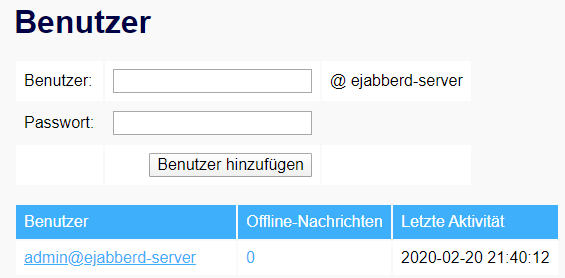
\includegraphics[width=\linewidth]{images/AdminPortalAddUsers}
\end{minipage}
\caption{Links Übersicht: Administrationsportal, rechts: Übersicht: Benutzerverwaltung, eigene Darstellung}
\label{img:AdminPortalEjabberdOverview}
\end{figure}

Mit einem Klick auf \texttt{Virtuelle Hosts} sieht man alle Domains, die auf dem ejabberd-Server registriert sind. Für dieses Projekt sieht man in der Übersicht die Domain \texttt{ejabberd-server} und die Anzahl der vorhandenen und aktuell angemeldeten Benutzer. Klickt man auf eine Domain und dann in der Auswahl auf \texttt{Benutzer}, können Benutzer verwaltet werden, siehe \autoref{img:AdminPortalEjabberdOverview} rechte Abbildung.

\subsubsection*{Konfiguration weiterer Module}

Welche weiteren Möglichkeiten es gibt, die Konfiguration von ejabberd sicherer und datenschutzfreundlicher zu machen, zeigt dieser Abschnitt auf.

Mit Shaper-Rules lassen sich unter anderem die maximale Anzahl an Verbindungen (Sessions) pro Benutzer einschränken.  

\bigskip

\begin{lstlisting}[language=yaml, caption={Anpassung der Shaper-Rules}]
shaper_rules:
  max_user_sessions: 10
  max_user_offline_messages:
    - 5000: admin
    - 500
\end{lstlisting}

Wie im Listing dargestellt, werden die Anzahl an Sessions pro Benutzer auf zehn verringert, um eine Überlastung des Servers und damit einen Systemausfall vorzubeugen. Zusätzlich wird die maximale Anzahl an Nachrichten, die der Server speichert, bis der Benutzer erneut online ist auf 500 reduziert. Diese Art von Nachrichten werden als Offline-Nachrichten bezeichnet. Die Anzahl an Offline-Nachrichten für den Benutzer \glqq admin\grqq mit 5000 Nachrichten ist vorkonfiguriert.

Ein weiteres wichtiges Modul ist \texttt{mod\_disco}. Dieses Modul erlaubt es, einem Client Kontaktinformationen zu zustellen, damit ein Benutzer Spam oder Missbrauch melden kann.

\bigskip

\begin{lstlisting}[language=yaml, caption={Kontaktinformationen für Spam- oder Missbrauchsmeldungen}]
mod_disco:
  server_info:
    -
      modules: all
      name: "abuse-addresses"
      urls:
        - "mailto:admin@mail.de"
    -
      modules: all
      name: "support-addresses"
      urls:
        - "mailto:admin@mail.de"
\end{lstlisting}

Das Listing zeigt wie in der Liste \texttt{server\_info} zusätzliche Informationen über den Server hinterlegt werden können. Ejabberd ünterstützt die \ac{XMPP}-Erweiterung \texttt{XEP-0157: Contact Addresses for XMPP Services}. Der Client sendet eine Anforderung über \ac{XMPP}. Der Server sendet dem Client die Kontaktinformationen zu. Der Client präsentiert dem Benutzer die Ergebnisse. Der genaue Ablauf ist in  \cite{xepContactInformation} beschrieben. Der Wert \texttt{all} bei \texttt{modules} bewirkt, dass die für alle Module, die ejabberd dem Client zur Verfügung steht, die Kontaktinformationen zugeordnet ist. Alternativ lässt sich eine Liste von bestimmten Modulen übergeben. Die Kontaktinformation ist dann nur für die in der Liste angegebenen Modulen abrufbar. Über den \texttt{url} Parameter lassen sich E-Mail Adressen oder bestimmte \ac{URI}s angeben.

Das Modul \texttt{mod\_last} protokolliert den Zeitpunkt, zu dem sich ein Client am System an- oder abmeldet. Im Sinne einer datenschutzfreundlichen Konfiguration wird das Modul durch Auskommentieren in der Konfigurationsdatei deaktiviert.

Für den Abschnitt Machine Learning in der Arbeit werden die Nachrichten benötigt, die sich Benutzer gegenseitig senden. Dafür ist eine Speicherung des Nachrichtenverlaufs notwendig. Zudem gibt es Clients, deren interner Speicherplatz zu gering ist, um Nachrichten selbst persistent zu speichern. Aus diesen Gründen kann das Modul \ac{MAM} aktiviert werden. Es ist in der \ac{XMPP}-Erweiterung \texttt{XEP-0313} spezifiziert.\cite{xepMAM}

Wichtige Funktionen von \ac{MAM} nach \cite{xepMAM}:

\begin{itemize}
\item Archivierung von Nachrichten auf dem Server
\item Archivierung der Nachrichten eines Multi-User-Chats (Gruppen-Chat)
\item Abruf der Nachrichten durch ein \ac{XMPP}-Query Request durch Clients
\item Synchronisation des Nachrichtenverlaufs zwischen mehreren Clients
\end{itemize}

\texttt{XEP-0313} spezifiziert viele weitere Funktionen, für die \ac{MAM} eingesetzt werden kann. In diesem Projekt wird jedoch nur die erste Funktion implementiert. Nach \cite{xepMAM} muss ein \ac{XMPP}-Server \ac{MAM} nicht zwingend bereitstellen und die Kontrolle über die Einstellungen kann der Betreiber des Servers festlegen. Das Protokoll erlaubt einem Benutzer aber auch, die Einstellungen für die Nachrichtenarchivierung selbst festzulegen, sodass dieser entscheiden kann, ob er Nachrichten auf dem Server archivieren möchte oder nicht. Ein Client, der diese XEP-Erweiterung unterstützt, informiert den Server über die Änderungen in den Einstellungen oder kann die aktuellen Einstellungen vom Server abfragen.\cite{xepMAM}

\newpage

\autoref{img:MAMGetRequest} zeigt typische Kommunikationsverläufe. Der Client sendet eine Anfrage vom Typ \texttt{get} mit seiner Benutzer-ID. Im Element \texttt{prefs} gibt er das Protokoll \ac{MAM} an. Darunter sind zwei mögliche Antworten des Servers abgebildet. Im ersten Fall unterstützt der Server \ac{MAM} und antwortet mit den aktuellen Einstellungen des Benutzers. Das \texttt{prefs}-Element muss vorhanden sein. Dieses enthält die konfigurierten Richtlinien für die Archivierung. Die Elemente \texttt{always} und \texttt{never} müssen immer im \texttt{prefs}-Element enthalten sein, auch wenn sie leer sind. Sie beinhalten eine Liste von \texttt{jid}-Elemente (Jabber-IDs). Für die Jabber-IDs im Element \texttt{always} ist die Archivierung immer aktiv. Für die IDs im Element \texttt{never} archiviert der Server niemals Nachrichtenverläufe. Im dritten Teilbild ist eine alternative Antwort des Servers an den Client dargestellt. Der Server antwortet mit einer \ac{XMPP}-Nachricht vom Typ \texttt{error} und dem Element \texttt{feature-not-implemented}, wenn er \ac{MAM} nicht unterstützt oder die Funktion deaktiviert ist.\cite{xepMAM}

\begin{figure}[h]
\centering
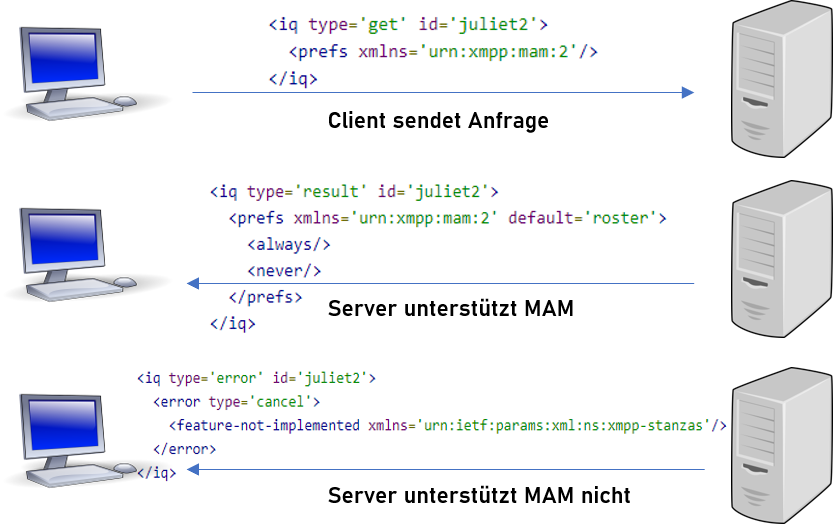
\includegraphics[width=.7\linewidth]{images/XEP0313_GetRequest}
\caption{Anfrage des Client zum Abruf der aktuellen \ac{MAM} Einstellungen \cite{xepMAM}, eigene Darstellung}
\label{img:MAMGetRequest}
\end{figure}

Der Autor von \cite{xepMAM} beschreibt, dass die Einstellungen der Archivierung mit einer Anfrage vom Typ \texttt{set} auch verändert werden können. Die Anfrage ist in \autoref{img:MAMUpdate} gezeigt.

\begin{figure}[h]
\centering
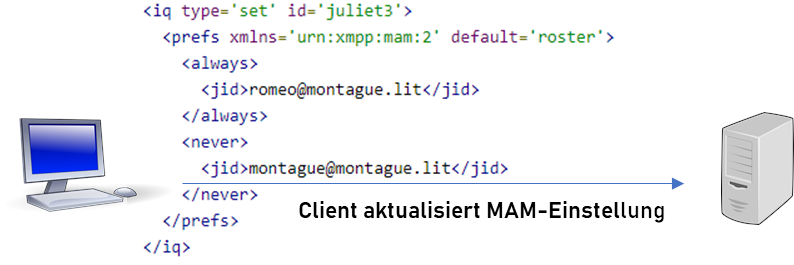
\includegraphics[width=.8\linewidth]{images/XEP0313_UpdateRequest}
\caption{Aktualisierung der Archivierungseinstellungen durch den Client \cite{xepMAM}, eigene Darstellung}
\label{img:MAMUpdate}
\end{figure}

Der Server speichert die Einstellungen nach Erhalt der Anfrage. Er archiviert von diesem Zeitpunkt alle Nachrichten für die Jabber-ID \texttt{romeo@montague.lit}. Für den Benutzer der ID \texttt{montague@montague.lit} werden keine Nachrichten mehr in der Datenbank gespeichert.

Das folgende Listing zeigt die Einstellungen für \ac{MAM} von ejabberd, die für dieses Projekt konfiguriert sind.

\bigskip

\begin{lstlisting}[language=yaml, caption={Konfiguration der Einstellungen für die Nachrichtenarchivierung}]
mod_mam:
    db_type: sql
    assume_mam_usage: true
    default: always
    request_activates_archiving: true
\end{lstlisting}

%TODO alle erwähnten Machine Learing Abschnitte noch konkret durch die Abschnittnummer ersetzen
Das Modul \texttt{mod\_mam} realisiert die zuvor beschrieben Funktionen von \ac{MAM}. Einerseits schreibt der Datenschutz vor, dass der Benutzer Kontrolle über seine Daten behalten muss, andererseits werden die Nachrichtenverläufe für den Abschnitt Machine Learning benötigt. Aus diesem Grund ist ein Kompromiss in der Einstellung festzulegen. Die Nachrichten sollen nur archiviert werden, wenn ein Benutzer das ausdrücklich veranlasst. Durch der aktivierten Einstellung \texttt{request\_activates\_archiving} speichert ejabberd nur dann Nachrichten, wenn der Client eine Anfrage sendet, die diese Archivierung aktiviert. Sendet ein Client diese Anfrage, werden ab diesem Zeitpunkt an alle Nachrichten des Client gespeichert. Mit \texttt{db\_type: sql} wird festgelegt, dass die Nachrichten in der in \autoref{sec:InstallationEjabberd} installierten MySQL Datenbank gespeichert werden.

Über das Modul \texttt{mod\_roster} kann vermieden werden, dass bei jedem Login die gesamte Kontaktliste (Roster) eines Benutzers erneut heruntergeladen werden muss. Das folgende Listing zeigt die Einstellungen.

\bigskip

\begin{lstlisting}[language=yaml, caption={Einstellungen des Moduls mod\_rosters}]
mod_roster:
  versioning: true
\end{lstlisting}

Dadurch wird die \ac{XMPP}-Erweiterung \texttt{XEP-0237: Roster Versioning} \cite{xep0237RosterVersioning} aktiviert und sorgt dafür, dass die Kontaktliste nur bei Änderungen erneut heruntergeladen werden muss. Das Verfahren spart damit Bandbreite ein.

Abschließend werden aus Sicherheitsgründen das Modul \texttt{mod\_version} und \texttt{mod\_http\_api} angepasst. Die Anpassungen sind in \autoref{lst:ejabberdImportantSecuritySettings} dargestellt.

\begin{lstlisting}[language=yaml, caption={Konfiguration relevanter Module für die Sicherheit von ejabberd},label={lst:ejabberdImportantSecuritySettings}]
mod_version: 
  show_os: false

## mod_http_api: {}
\end{lstlisting}

Ein Client kann die Version des Betriebssystems, auf dem ejabberd installiert ist, grundsätzlich abfragen. Das wird durch die Einstellung \texttt{show\_os: false} verhindert. Ebenfalls wird das Modul \texttt{mod\_http\_api} deaktiviert. Eine Administration über das \ac{HTTP} ist damit nicht möglich. Die ejabberd-Instanz kann nur noch über das erlang Kommandozeilenprogramm \texttt{ejabberdctl} verwaltet werden, siehe \autoref{lst:AddAdminUserEjabberd}.

Nun ist ejabberd für den Gebrauch in der Projektarbeit konfiguriert. Der Server kann nun von jedem beliebigen \ac{XMPP}-Client genutzt werden.

\newpage

\section{Entwicklung des Chat-Clients}
\label{sec:ClientEntwicklung}

\subsection{Entwicklung der GUI}
\label{subsec:EntwicklungGUI}
Einleitend wurde im \autoref{subsec:GuiPython} auf die Möglichkeiten einer grafischen Benutzeroberfläche mit Python eingegangen. Mit dem Resultat der Entscheidungsmatrizen aus \autoref{tab:EntscheidungsmatrixFrameworkart} und \autoref{tab:EntscheidungsmatrixWebFramework} erfolgt die Umsetzung mithilfe der in \autoref{sec:Benutzeroberfläche} erläuterten Werkzeuge einer Webentwicklung. Für die Entwicklung eines Web-Frontends %TODO vllt Quelle reinbringen
bildet eine Rahmenstruktur die Basis der Webseite. Der Rahmen bezieht sich dabei auf ein einzelnes \ac{HTML}-Dokument. Um nun auf den \ac{HTML}-Aufbau der Webseiten einzugehen ist das Verständnis über die Verknüpfung und Auslieferzeitpunkten der Einzelseiten relevant. Für diese Verknüpfung können die nachfolgenden Abbildungen betrachtet werden.
\begin{figure}[h]
	\begin{minipage}[c]{.4\textwidth}
		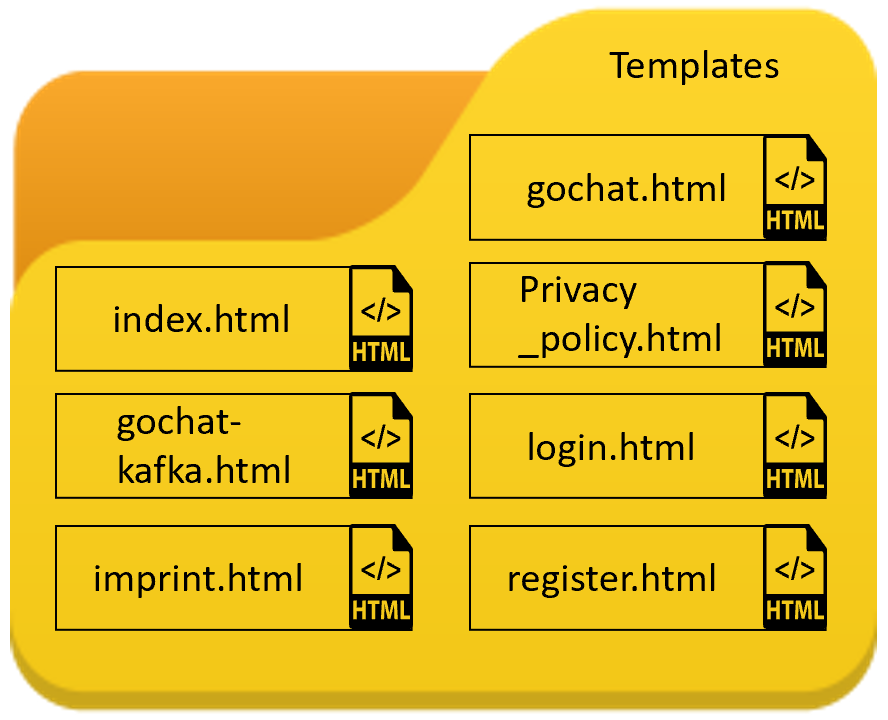
\includegraphics[width=\textwidth]{images/HTMLDateienOrdner}
		\caption{Zugriff über ID, eigene Darstellung}
		\label{img:HTMLDateienOrdner}
	\end{minipage}
	\hspace{0.05\linewidth}% Abstand zwischen Bilder
	\begin{minipage}[c]{.4\textwidth}
		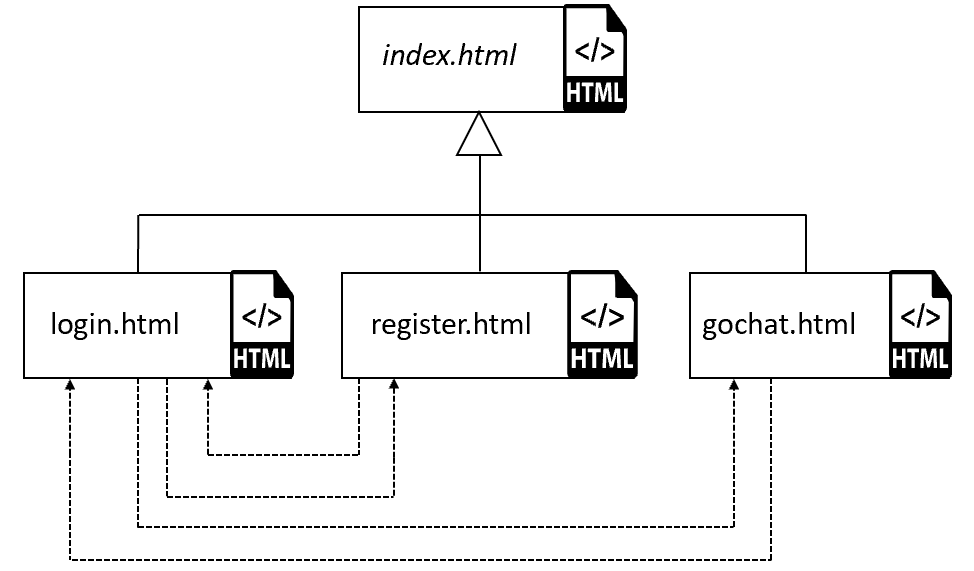
\includegraphics[scale=0.7]{images/HTMLDateienAufrufbaum}
		\caption{Zugriff über Klasse, eigene Darstellung}
		\label{img:DateinAufrufbaum}
	\end{minipage}
\end{figure}
\autoref{img:HTMLDateienOrdner} zeigt welche HTML-Dateien für die Applikation relevant sind und wo diese in der Ordnerstruktur zu finden sind. Die zweite \autoref{img:DateinAufrufbaum} zeigt wie die Seiten gegenseitig benötigt werden. Hierbei handelt es sich nicht um den Source-Code sondern um die Aufrufstruktur für den Nutzer. Mit der \textit{index.html} in kursiver Schrift wird angedeutet, dass kein Nutzer diese Seite ausgeliefert bekommt. Dieses \ac{HTML}-Dokument dient lediglich als Basis. Die weiteren Dateien erben den Inhalt der index.html, was die UML-Notation andeuten soll. Auf der zweiten Ebene hat der Nutzer die Möglichkeit zwischen den Dateien, welche hinter einer Route liegen, zu wechseln, je nach Verwendung. Mit dem Verständnis über die Beziehungen der Dateien wird im Folgenden auf den \ac{HTML}-Aufbau der einzelnen HTML-Dokumenten eingegangen.


\subsubsection*{Strukturaufbau der Webseiten}
\label{subsubsec: StrukturaufbauWebseiten}
Eine Struktur als Rahmen der Webseite basiert grundlegend auf die Verwendung von \ac{HTML}. Für die Webseite bedeutet dies, dass die Struktur aus div-Boxen, welches ein \ac{HTML}-Elementen darstellt, besteht. Die div-Box kann den Tags, welche in \autoref{sec:HTMLCSSJS} erläutert wurden, zugeordnet werden, und bildet dadurch eine weitere Variante der \ac{HTML}-Tags. Grundsätzlich basiert eine Webseite auf einer index.html Datei, welche als Ausgangspunkt für den ersten Aufruf eines Nutzers dient. Bezogen auf die Struktur gibt es bei der Web-Entwicklung lediglich Vorschläge wie eine Umsetzung erfolgen kann, dennoch ist das Konzept nach eigenen Anforderungen zu definieren. Demnach kann eine Webseite komplett in der \textbf{index.html} Datei ausgeliefert werden, oder für jede Route, die der Nutzer adressieren kann, wird eine neue \ac{HTML}-Datei ausgeliefert. Im Rahmen der Studienarbeit wird das zweite Konzept verfolgt, weshalb die index.html Datei lediglich als Basis für eine einheitliche Struktur dient. Dieses Konzept ist in der \autoref{img:DateinAufrufbaum} dargestellt. Außerdem ist daraus ersichtlich, dass die index.html nicht direkt ausgeliefert wird. Wie die nachfolgende \autoref{img:index-struktur} zeigt, bildet der nav-Tag das Konstrukt welches der Hauptbestandteil der index-Seite darstellt.
\begin{figure}[h]
	\centering
	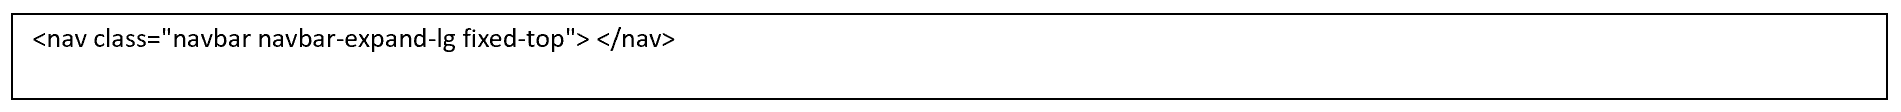
\includegraphics[width=\linewidth]{images/indexbody}
	\caption{Basis-Konstrukt der Index-Seite, eigene Darstellung}
	\label{img:index-struktur}
\end{figure}
Der nav-Tag wird unter der Verwendung einer Navigationsleiste in HTML5 benutzt. Das Konstrukt ist Teil der index-Datei, um eine einheitliche Navigationsleiste für jede weitere Webseite zu definieren. Des Weiteren sind dieser Leiste HTML-Elemente zuzuordnen. Der strukturelle Aufbau mit den Ergänzung an dem Basis-Konstrukt ist in der folgenden \autoref{img:index-strukturInhalt} dargestellt.
\begin{figure}[h]
	\centering
	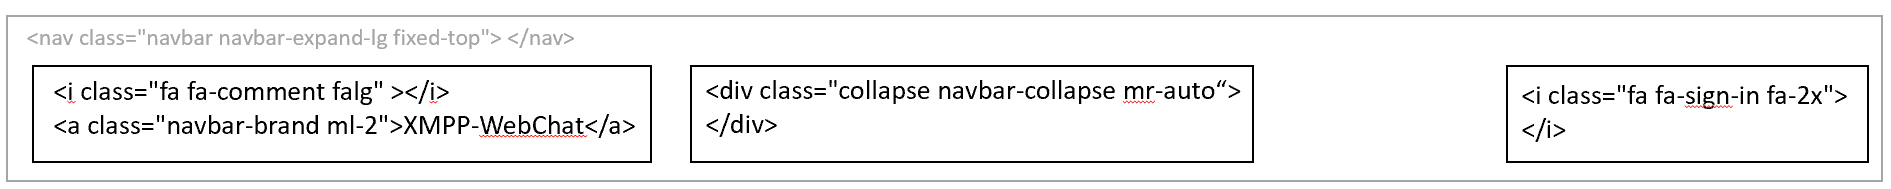
\includegraphics[width=\linewidth]{images/indexbodyInhalt}
	\caption{Erweiterung der Navigationsleiste um weitere HTML-Elemente, eigene Darstellung}
	\label{img:index-strukturInhalt}
\end{figure}\\
Die Erweiterungen beinhalten zwei i-Tags, welche Icons darstellen bzw. hervorheben sollen. Der a-Tag definiert eine Referenz in Form eines Hyperlinks, welcher zu einer angegebenen Seite verzweigen kann. Grundidee ist hierbei die Verzweigung des Logos auf die index-Seite bzw. auf die Webseite, die der Nutzer als home-Seite betrachten soll. Die div-Box als letztes Element der Index-Seite beinhaltet weitere Elemente, die keine Relevanz für den Strukturaufbau der Webseite darstellt. Diesem Element sind überwiegend weitere Links und Textfelder zugeordnet, wie es der \autoref{img:Navbar} zu entnehmen ist. Den \ac{HTML}-Elementen kann mithilfe von \ac{CSS} gestalterische Aspekte verliehen werden. Diese Aufgabe kann das unter \autoref{sec:HTMLCSSJS} vorgestellte Framework namens Bootstrap übernehmen. Dies ist mitunter der Grund weshalb den \ac{HTML}-Elementen solche Klassennamen gegeben werden. Bezogen auf diese definierten Klassennamen kann durch einbinden der bootstrap.css Datei im header die definierten Styles verwendet werden. Mit kleinen Ergänzungen stellt die \autoref{img:Navbar} die vollständige index-Seite dar.
\begin{figure}[h]
	\centering
	
\includegraphics[width=\linewidth]{images/indexHTML&CSS}
	\caption{Webbrowserdarstellung der Index-Seite, eigene Darstellung}
	\label{img:Navbar}
\end{figure}\\
Aufbauend auf der Index-Seite können alle weiteren Webseiten die Navigationsleiste über die index.html Datei erben, wie es das Konzept aus \autoref{img:DateinAufrufbaum} darstellt. Dadurch kann eine durchgängige Struktur beibehalten werden. Die Index-Seite bildet daher keine Möglichkeit durch einen Nutzer direkt adressiert zu werden. Die erste Anlaufstelle eines unangemeldeten Nutzers wird durch die Login-Seite abgebildet. Unabhängig von der Navigationsleiste bietet die \textbf{login.html} Datei ein Formular für den Anmeldevorgang. Mithilfe von Bootstrap wird die Basis-Struktur durch div-Boxen und Klassennamen definiert, wie sie der folgenden \autoref{img:BasisStrukturLogin} zu entnehmen sind.
\begin{figure}[h]
	\centering
	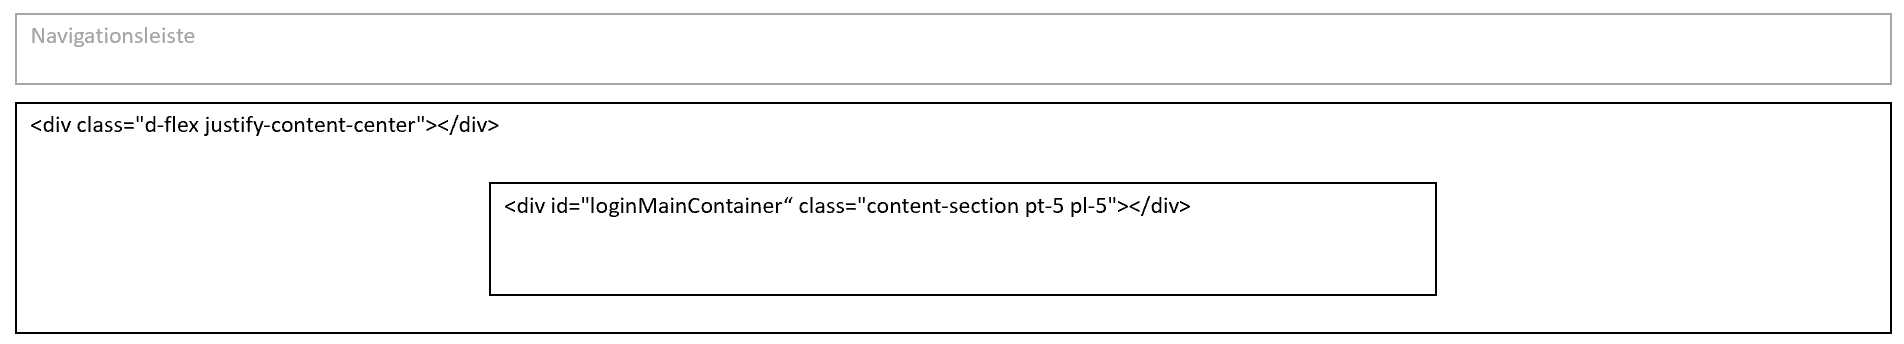
\includegraphics[width=\linewidth]{images/loginBasisStruktur}
	\caption{Basis-Struktur der login-Seite, eigene Darstellung}
	\label{img:BasisStrukturLogin}
\end{figure}
Basierend auf diesem Aufbau bildet die Klasse \textit{d-flex justify-content-center} die Möglichkeit weitere div-Boxen flexibel anzuordnen. Eine Variante wie sie in \autoref{sec:HTMLCSSJS} unter \ac{CSS} erläutert wurde. Die \autoref{img:BasisStrukturLogin} bildet noch kein Formular der Login-Seit ab, sondern lediglich Container für eine korrekte Anordnung. Im Folgenden wird der div-Box mit der Klasse \textit{content-section pt-5 pl-5} ein form-Tag hinzugefügt, um in Kooperation mit Bootstrap ein Formular, bezogen auf die Anmeldung, zu konstruieren.
\begin{figure}[h]
	\centering
	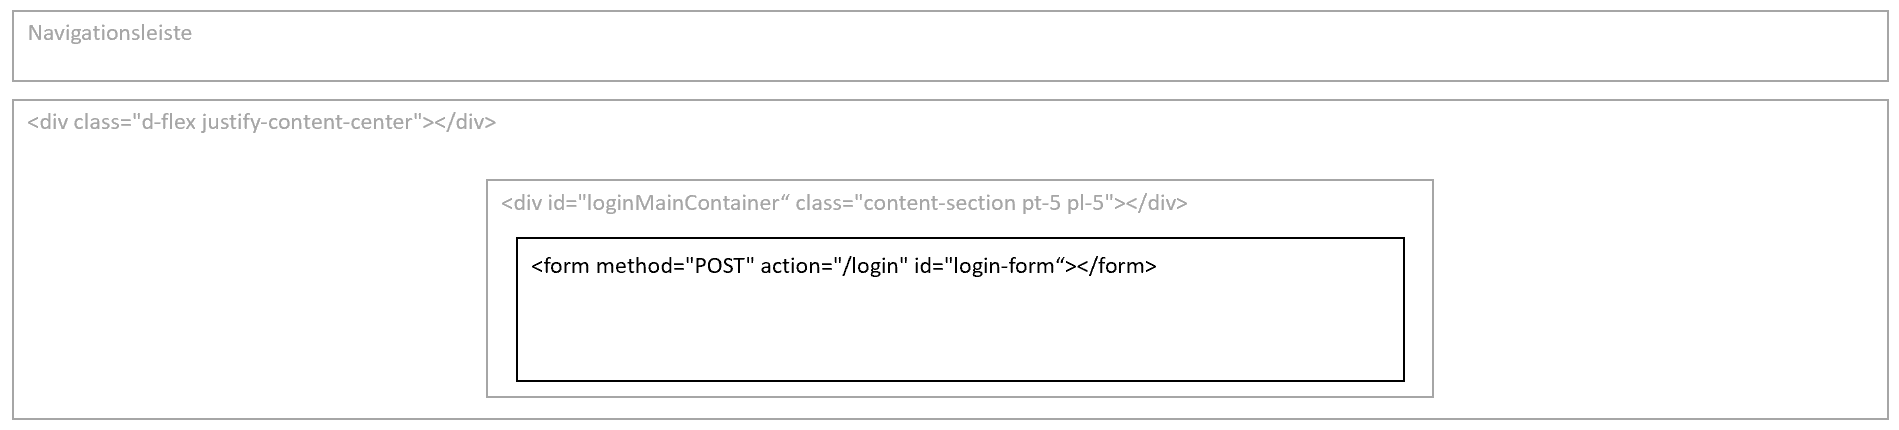
\includegraphics[scale=0.55]{images/loginBasisStruktur&FormContainer}
	\caption{Integration des Formular-Tags in die Login-Basisstruktur, eigene Darstellung}
	\label{img:BasisStrukturLoginUnd Formular}
\end{figure}\\
Die Design-Elemente werden über der bootstrap.css Datei dem Formular mitgegeben. Der strukturelle Aufbau der Login-Seite ist damit vollendet. Für das Formular werden dem form-Container Textfelder, Buttons und ähnliches hinzugefügt, welche das Formular gestalterisch vervollständigen. Diese Elemente sind in der \autoref{img:LoginSeiteVollständig} dargestellt. Außerdem bildet die \autoref{img:LoginSeiteVollständig} die vollständige Login-Seite ab, wobei dieser Webseite eine weitere div-Box zugeteilt wird, welches für die Struktur keine Relevanz darstellt und daher nicht aufgeführt wurde.
\begin{figure}[h]
	\centering
	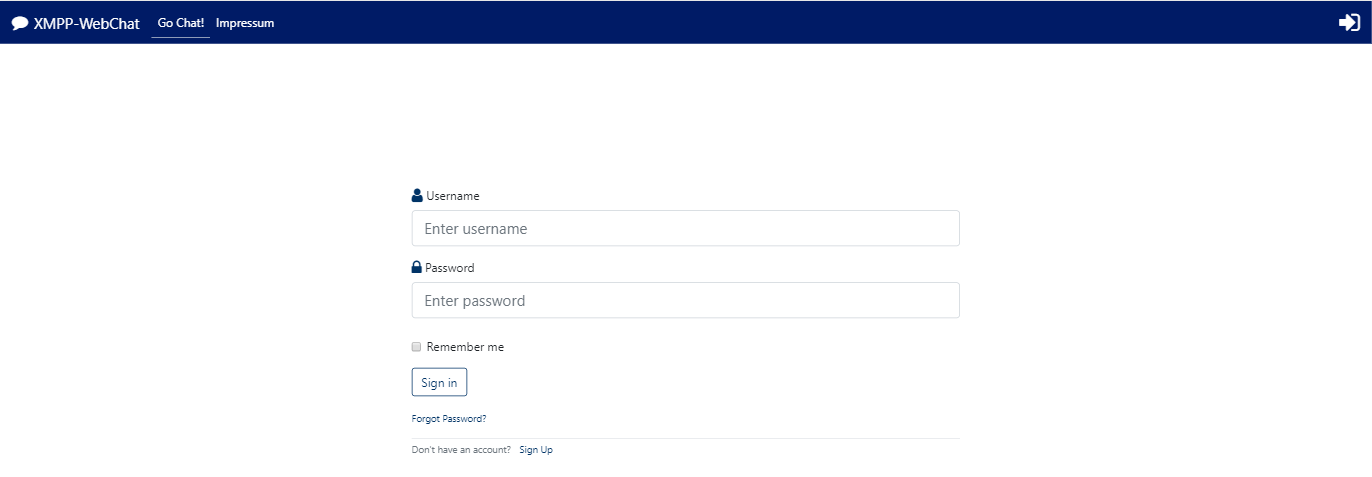
\includegraphics[width=\linewidth]{images/loginSeiteFertig}
	\caption{Vollständige Login-Seite, eigene Darstellung}
	\label{img:LoginSeiteVollständig}
\end{figure}
Aufgrund der Ähnlichkeit der \textbf{Registrierungs-Seite} zur Login-Seite erfolgt dafür keine detaillierte Erläuterung sondern lediglich die Darstellung der strukturierten Webseite mit den HTML-Inhalten und der Designdarstellung dieser Route. Einziges unterscheidendes Merkmal zur Login-Seite sind die HTML-Elemente innerhalb des Formulars, welche sich vor allem in der Anzahl unterscheiden. Die folgende \autoref{img:RegisterSeiteVollständig} zeigt sowohl die Struktur als auch die Darstellung für den Nutzer.
\begin{figure}[h]
	\centering
	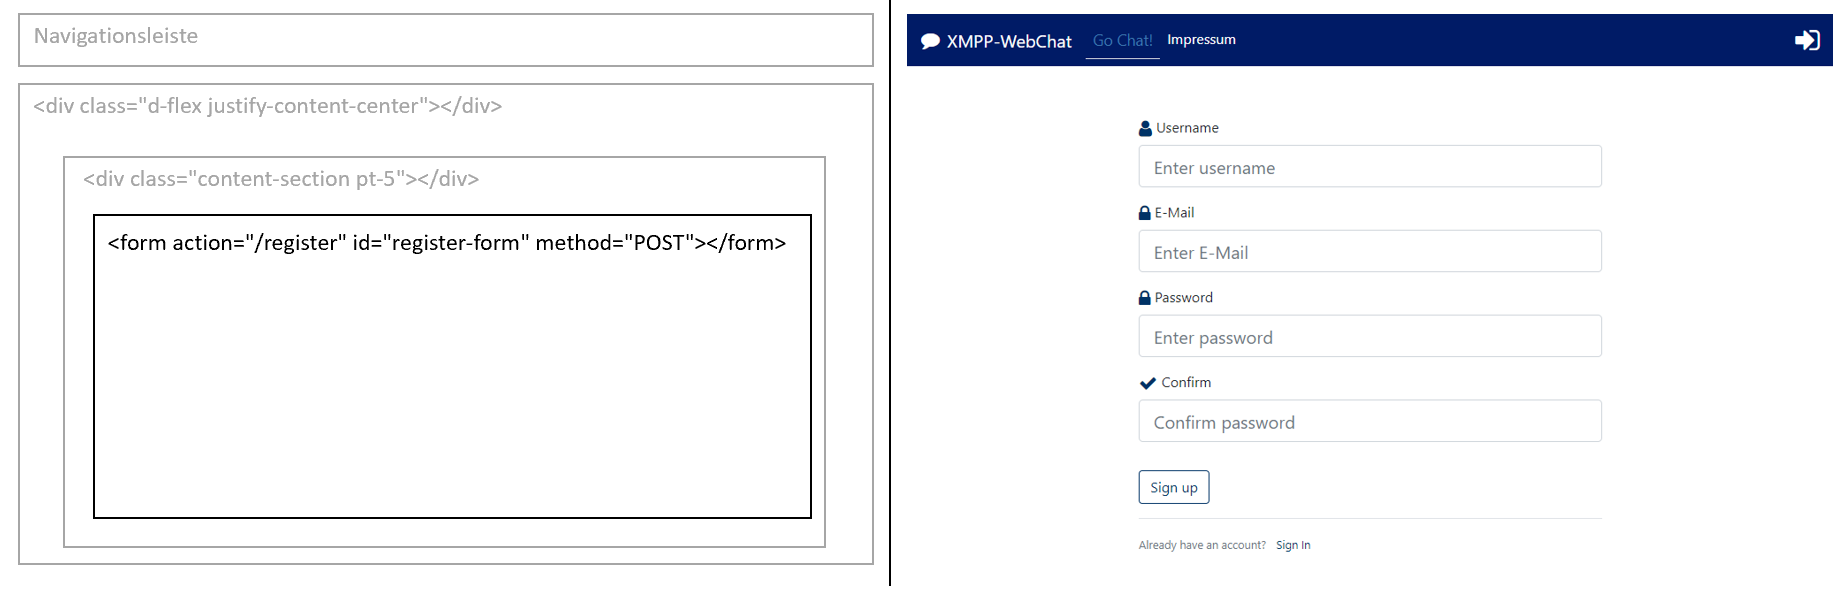
\includegraphics[width=\linewidth]{images/RegisterPage}
	\caption{Vollständige Registrierungs-Seite, eigene Darstellung}
	\label{img:RegisterSeiteVollständig}
\end{figure}
Aus der \autoref{img:RegisterSeiteVollständig} sind die erwähnten Unterschiede nicht zu entnehmen, da Sie keine Einwirkung auf die Grundstruktur der Registrierungsseite haben und daher wurden diese nicht mit in die form-Box aufgenommen. Die Hauptseite des Web-Clients wird dem Nutzer durch die \textbf{gochat.html} Datei ausgeliefert. Wie der \autoref{img:DateinAufrufbaum} zu entnehmen ist, kann der Nutzer die Seite von der login.html Seite erreichen. Dabei handelte es sich um einen normalen Anmeldevorgang. Die gochat.html Datei beinhaltet den Aufbau des Chats sowie zahlreiche weitere Funktionen welche dem Nutzer nur angeboten werden wenn er angemeldet ist. Ein Securityaspekt, welcher im routing geregelt wird und kein Bestandteil der HTML-Dokumente ist. Die gochat.html Datei gliedert sich in mehrere HTML-Tags bzw. in mehrere div-Boxen, auf die im einzelnen detaillierter eingegangen wird. Dafür stellt die erste \autoref{img:BasisStruktur1Gochat} eine Art erste Ebene dar, welche die einzelnen Elemente voneinander abgrenzt und eine Struktur für die Teilbereiche bildet.
\begin{figure}[h]
	\centering
	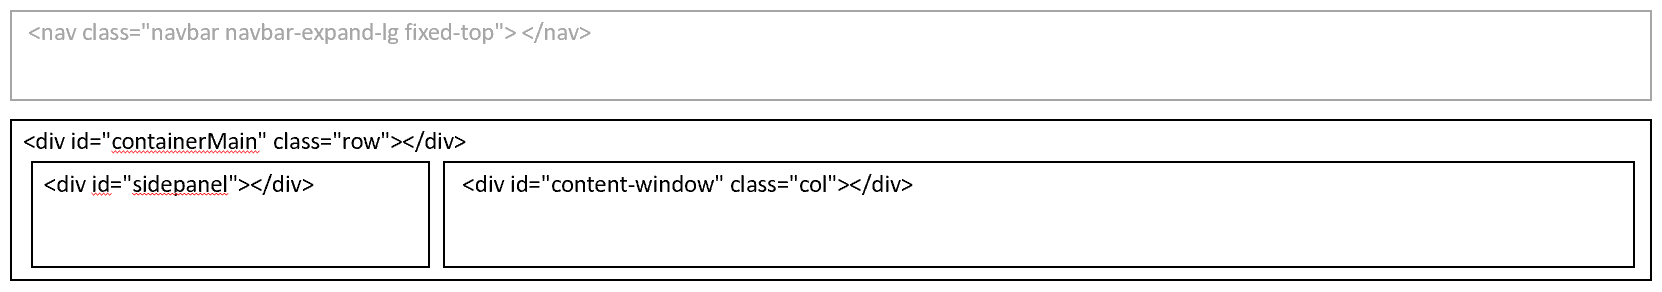
\includegraphics[width=\linewidth]{images/BasisStruktur1Gochat}
	\caption{Strukturierung von gochat.html auf der ersten Ebene, eigene Darstellung}
	\label{img:BasisStruktur1Gochat}
\end{figure}
Die ausgegraute div-Box mit der Klasse \textit{navbar} wird ausschließlich für die Vollständigkeit mitaufgeführt. Die Klasse ist Teil der index.html und wird von gochat.html geerbt. Dadurch besteht die erste Ebene aus den drei anderen div-Boxen. Die erste div-Box mit der id \textit{containerMain} deckt den gesamten Viewport der Webseite ab. Dadurch ergibt sich die Möglichkeit innere Container entsprechend des Viewports anzupassen.\\
Ein relevantes Merkmal ist dabei die Klasse \textit{row}, welches Bestandteil von Bootstrap ist. Die Klasse kann in mehreren Situationen zum Einsatz kommen. Im Fall von der gochat.html handelt es sich um das Grid-System von Bootstrap. Dieses bietet die Möglichkeit Container bzw. div-Boxen in dem von Bootstrap spezifizierten Grid auszurichten. Dadurch wird dem Anwender die Möglichkeit geboten eine row zu definieren und diese, wie die nachfolgende Abbildung zeigt, in columns zu unterteilen.
\begin{figure}[h]
	\centering
	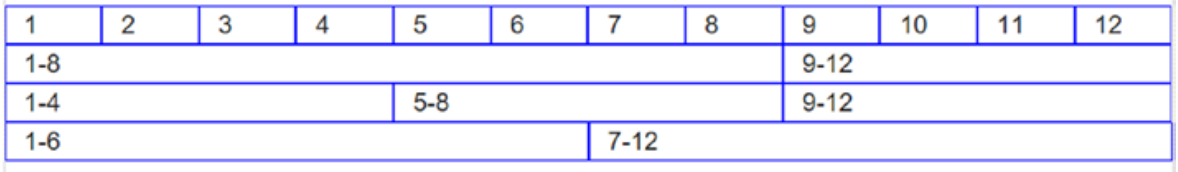
\includegraphics[scale=0.9]{images/GridSystem}
	\caption{Das Grid System von Bootstrap, \cite{krause2016introducing}}
	\label{img:GridSystem}
\end{figure}
Mit diesem Konzept können die Inhalte problemlos aneinander gereiht bzw. angeordnet werden. \cite{krause2016introducing}\\
Aufgrund dieser Konzeptionierung wird der id \textit{content-window} die Klasse \textit{col} zugeordnet. Damit wird gewährleistet, dass sich die div-Box wie eine Spalte anordnet. Die Anordnung kann außerdem über eigene CSS-Styles definiert werden, wie es bei dem Sidepanel der Fall ist. Da die CSS keine detaillierte Auswirkung auf die Struktur hat wird auf diese Styles nicht genaueres eingegangen. Im Folgenden soll das Sidepanel mit seinem Container im Vordergrund stehen. Um die innere Struktur zu definieren sind die Aufgaben bzw. die Anzeigemöglichkeiten des Sidepanels zu definieren. Entsprechend der Aufgaben können Boxen angelegt werden welche den Inhalt im weiteren Verlauf spezifizieren. Demnach sind folgende Bestandteile:
\begin{itemize}
	\item Profilanzeige
	\item Suchfunktion innerhalb der eigenen Kontaktliste
	\item Kontaktliste für Einzel- und Gruppenchats
	\item Zusätzliche Optionen
\end{itemize}
relevant für das Sidepanel. Zur Integration in die gochat.html wird für jedem Bestandteil einen eigenen Container definiert. Diese werden dem Sidepanel zugeordnet, wie es auf der nachfolgenden Abbildung dargestellt ist.
\begin{figure}[h]
	\centering
	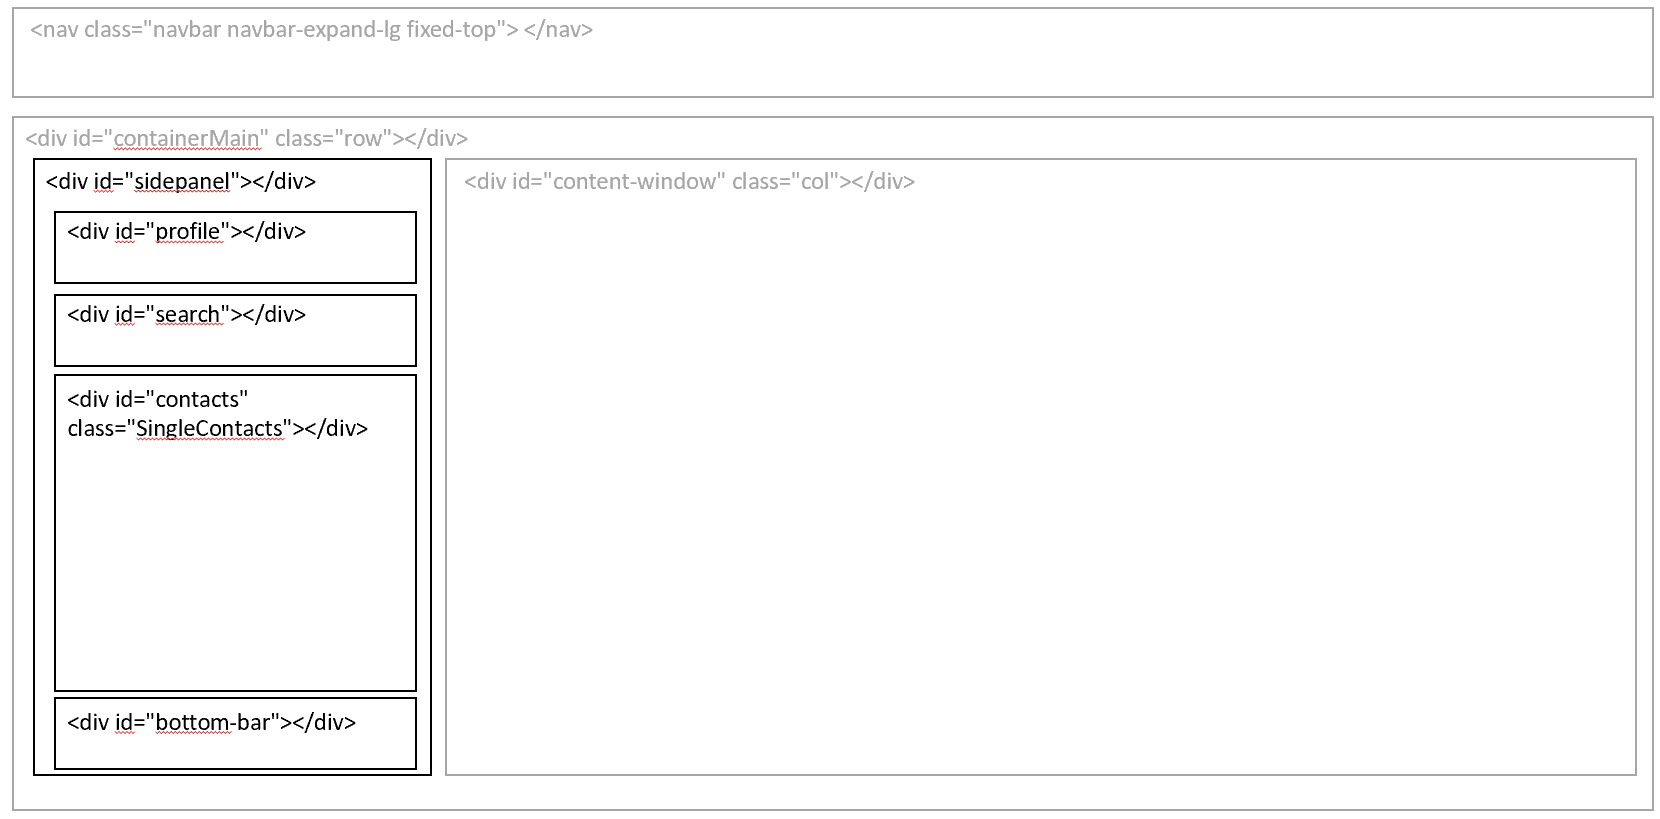
\includegraphics[width=\linewidth]{images/BasisStruktur1GochatSidepanel}
	\caption{Erweiterung des Sidepanels um die aufgezählten Bestandteile, eigene Darstellung}
	\label{img:Sidepanel}
\end{figure}
Die eigenständigen Container bietet die Möglichkeit die Elemente getrennt voneinander zu gestalten. Außerdem kann dadurch den Elementen im weiteren Verlauf dynamische Aspekte zugeteilt werden. Damit steht die Struktur des Sidepanels. Den einzelnen Containern können weitere HTML-Elemente zugeordnet werden. Das bedeutet eine tiefere Verschachtelung, die nicht nähers erläutert wird. Lediglich auf Elemente welche der Nutzer sehen kann soll kurz dargestellt werden. Für die id \textit{profile} bedeutet das, ein img-Tag für das Profilbild und ein p-Tag für den Namen des Nutzers.\\
Der \textit{search}-Box kann ein Inputfield zugeordnet werden, welches dem Nutzer die Möglichkeit bietet Texte einzugeben. \cite{bootstrapOnline}\\
Für \textit{contacts} gibt es keine erwähnenswerte Inhalte. Mit der Umsetzung der zusätzlichen Optionen wird der \textit{bottom-bar} zwei Buttons zugeteilt, welche diese Optionen bereitstellen sollen. Für die div-Box mit der id \textit{content-wndow} ist die Vorgehensweise identisch um alle Aufgabenbereiche, aus den Anforderungen, in der grafischen Benutzeroberfläche abzudecken. Diesem Container müssen daher folgende Bestandteile zugeordnet werden.
\begin{itemize}
	\item Profilanzeige des Chatpartners
	\item Nachrichtenansicht
	\item Möglichkeit eine Nachricht einzugeben (Textfeld)
\end{itemize}
In Abhängigkeit dieser definierten Bestandteile wird jedem ein Container zugeteilt, der die definierten Aufgaben innehalten soll.
\begin{figure}[h]
	\centering
	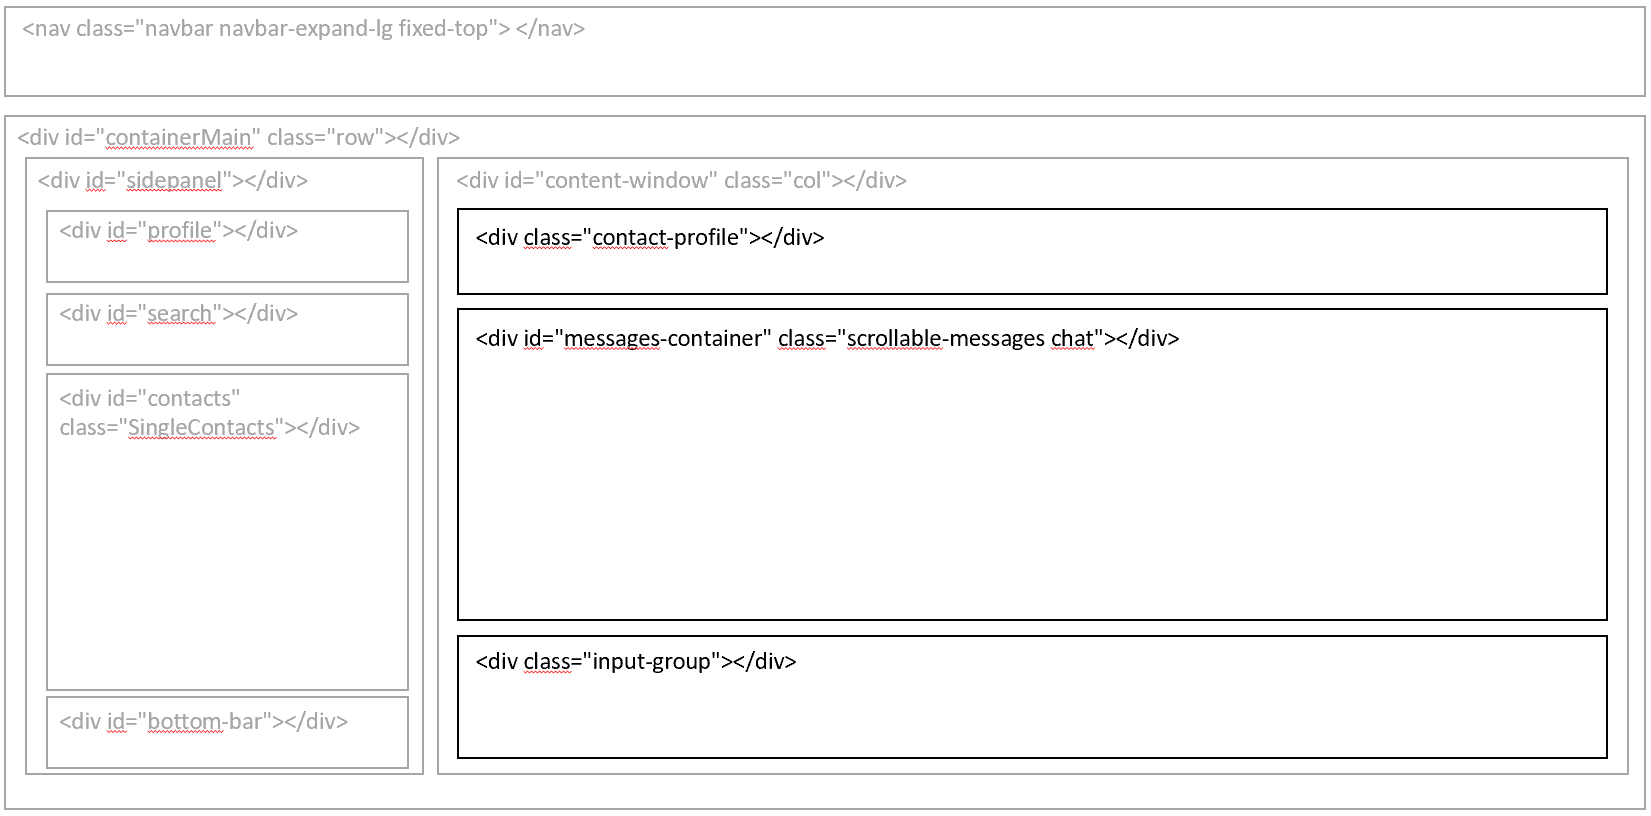
\includegraphics[width=\linewidth]{images/BasisStruktur1GochatContentWindow}
	\caption{Erweiterung des Containers \textit{content-window} um die aufgezählten Bestandteile, eigene Darstellung}
	\label{img:Content-window}
\end{figure}
Der Klasse \textit{contact-profil} sind die gleichen HTML-Elemente untergeordnet wie es schon bei der div-Box \textit{profile} der Fall war. Ergänzend dazu ist dem Kontaktprofil des Chatpartners ein Dropdownmenü zugeteilt, welches weitere Optionen bereitstellen soll. Für die Struktur von gochat.html werden diese Unterpunkte nicht benötigt. Außerdem ist das Dropdownmenü überwiegend ein CSS-Element, weshalb es kein wichtiger Aspekt in der Struktur darstellt. Der Container mit der id \textit{messages-container} bildet lediglich einen Rahmen um die Nachrichten des Chats, weshalb der Container keine weiteren HTML-Elemente aufzeigt. Die Nachrichten entstehen zur Laufzeit und sind daher kein Bestandteil der Struktur. Das Hauptmerkmal der Klasse \textit{input-group} ist das Textfeld und der Button, welches es innehat. Dadurch wird dem Nutzer gewährleistet seine Nachrichten einzugeben und über ein Button zu senden. Weitere HTML-Elemente spielen in der Struktur keine Rolle und sind daher nicht weiters aufgeführt. Alle Elemente, welche die Struktur der gochat.html Datei beschreiben sind in der \autoref{img:Content-window} aufgeführt. Unter der Verwendung von Bootstrap und eigenen Styles zeigt die \autoref{img:GochatUserview} die Hauptseite aus der Sicht des Nutzers.
\begin{figure}[h]
	\centering
	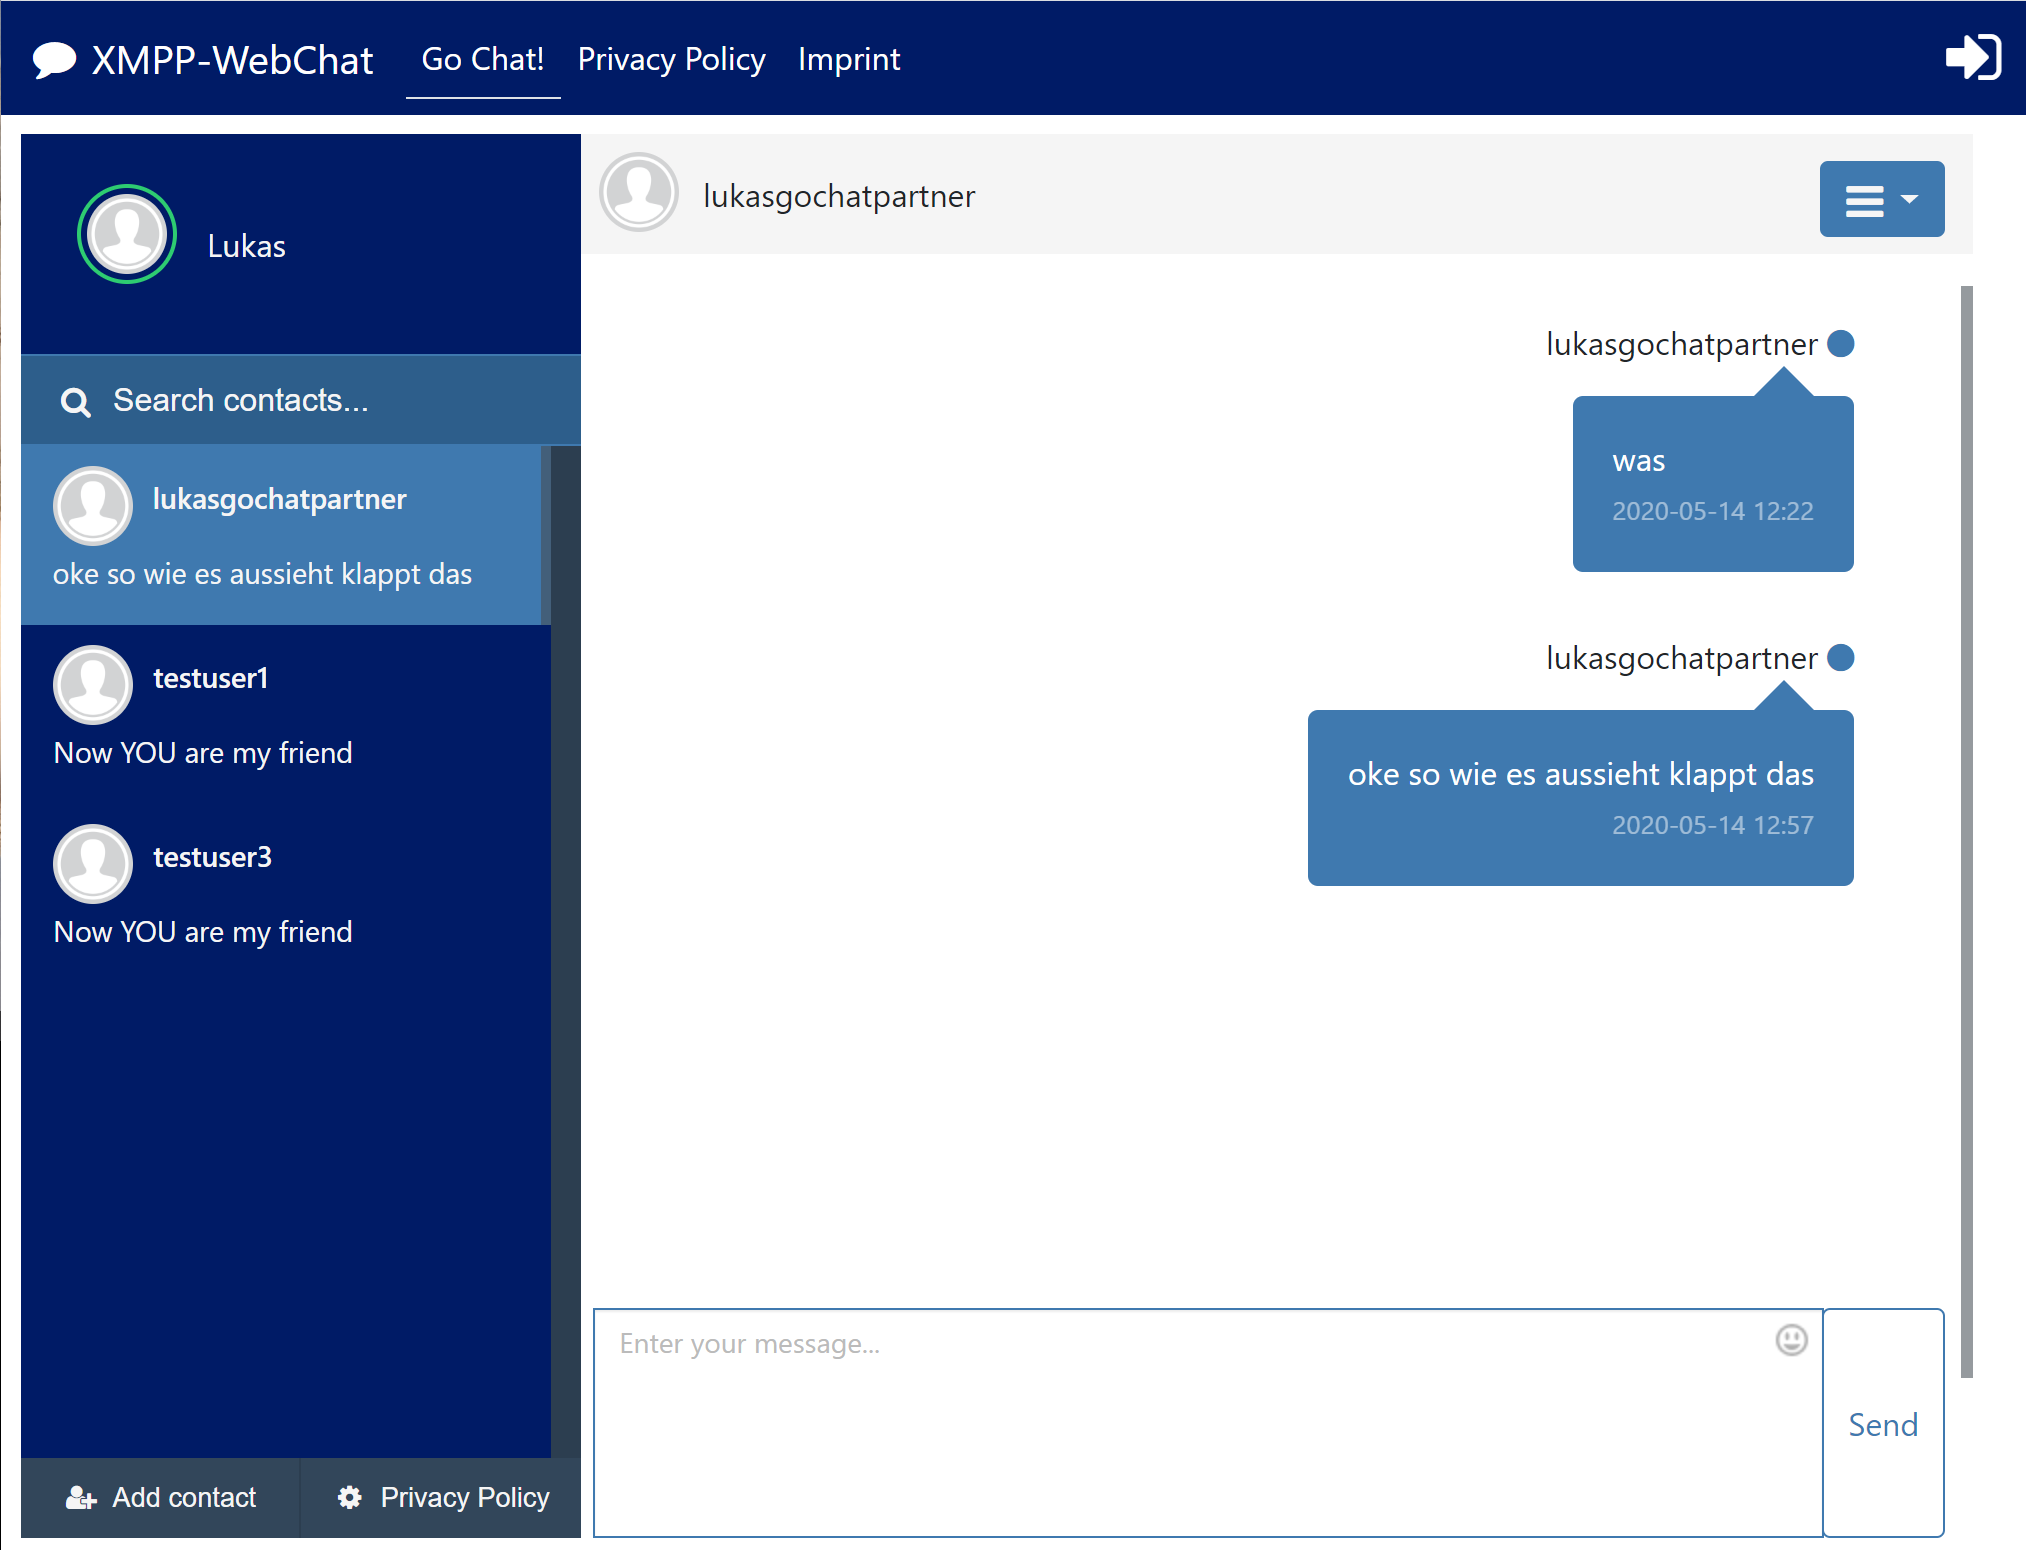
\includegraphics[width=\linewidth]{images/GochatUserAnsicht}
	\caption{gochat.html aus Sicht des Nutzers, eigene Darstellung}
	\label{img:GochatUserview}
\end{figure}
Mit der fertigen Struktur von gochat.html wurden alle Webseiten, die der Webserver ausliefert, erläutert. Das Erscheinungsbild, wie es bspw. in \autoref{img:GochatUserview} dargestellt ist entsteht hauptsächlich unter der Verwendung von \ac{CSS}. Diese Details werden aufgrund der Redundanzen und der Ähnlichkeit zu den Beispielen aus \autoref{sec:HTMLCSSJS} nicht nähers erläutert und können dem Source-Code entnommen werden. Eine größere Relevanz spielen die dynamischen Elemente, welche das Nutzerverhalten direkt beeinflussen können. Aus diesem Grund wird der JavaScript Code mit Bezug zur jeweiligen HTML-Datei detaillierter erläutert.

\subsubsection*{Integration dynamischer Elemente in die Webseiten}
\label{subsubsec:DynamischeElementeWebseiten}


\subsection{Implementierung des Backends}
\label{subsec:Backend}

\newpage

\chapter{Datenanalyse}
\label{chap:Datenanalyse}

\newpage

\chapter{Ergebnis}
\label{chap:Ergebnis}

\newpage

\chapter{Fazit}
\label{chap:Fazit}


\end{onehalfspacing}
\newpage

\bibliography{Literatur}
\newpage
%setze Anhang mit appendix
%addpart, sodass Anhang im Inhaltsverzeichnis ohne Buchstaben auftaucht
\appendix
\addpart{Anhang}

\chapter{Installation eines Apache Kafka Systems}
\label{InstallationKafka}

Die nachfolgende Anleitung bezieht sich auf die Installation eines Kafka-Systems. Die Installationsanleitung beschreibt alle notwendigen Schritte, um einen Server mit der \textbf{Kafka Version 2.4.0} in Betrieb zu nehmen. Die Anleitung beschreibt nicht, wie ein Cluster-System, welches einen Verbund mehrerer Kafka-Instanzen darstellt, in Betrieb genommen werden kann. Ziel ist es, eine einfache Installation aufzuzeigen und Kafka als Service auf einem Server bereitzustellen ohne, dass für die Ausführung der Kafka-Instanz ein Benutzer angemeldet sein muss. Die Informationen und Befehle sind aus der Kafka-Dokumentation \cite{kafkaDoc} zu entnehmen.

\bigskip

\textbf{Voraussetzungen:}

\smallskip

\begin{itemize}
\item Linux Ubuntu 18.04 LTS
\item Server
\begin{itemize}
\item mindestens 4GB RAM, empfohlen 8GB (Installation mit weniger RAM kann zu Problemen beim Start von Kafka führen, weil die Java Virutal Machine (JVM) eine \glqq OutOfMemory\grqq -Exception werfen kann.
\end{itemize}
\item OpenJDK 8 (Kafka ist in der Programmiersprache Java programmiert und benötigt deshalb eine lauffähige JVM.)
\end{itemize}

\section{Schritt 1: Anlegen eines Benutzers}

Für die Erstellung eines Benutzers muss sich auf dem Server mit einem Benutzer eingeloggt werden. Mit folgendem Kommando wird ein Benutzer mit dem Namen Kafka angelegt. Mit dem zweiten Kommando wird der Benutzer der \glqq sudo\grqq -Gruppe hinzugefügt und ist ab diesem Zeitpunkt berechtigt höher privilegierte Befehle auszuführen. Das letzte Kommando legt ein Passwort an, dass bei der Ausführung höher privilegierter Befehle abgefragt wird.

\smallskip

\begin{lstlisting}[language=Bash]
$ sudo adduser kafka # Benutzer anlegen
$ sudo adduser kafka sudo # Benutzer zur sudo-Gruppe hinzufügen
$ sudo passwd kafka # Anlegen eines sudo-Passwords
\end{lstlisting}

Anschließend muss sich mit dem neu erstellten Benutzer eingeloggt werden (Kommando: su kafka).

\section{Schritt 2: Installation der benötigten Komponenten}


Als nächstes muss das komprimmierte Kafka-Binary heruntergeladen werden. Hierzu kann das \textbf{curl}-Kommandozeilentool verwendet werden, um das Binary direkt aus dem Internet herunterzuladen und im Home-Verzeichnis des kafka-Benutzers gespeichert werden.

\smallskip

\begin{lstlisting}[language=Bash]
$ curl "http://mirror.checkdomain.de/apache/kafka/2.4.0/kafka_2.12-2.4.0.tgz" -o ~/kafka_2.12-2.4.0.tgz
\end{lstlisting}

Falls OpenJDK 8 noch nicht installiert ist, muss folgender Befehl ausgeführt werden.

\smallskip

\begin{lstlisting}[language=Bash]
$ sudo apt-get install openjdk-8-jdk
\end{lstlisting}

Erstellen Sie ein Grundverzeichnis in dem alle Kafka-Komponenten extrahiert werden können. Legen Sie mit folgendem Befehl ein Verzeichnis mit dem Namen \glqq kafka\grqq an. Extrahieren Sie die komprimierte Datei in dasselbe Verzeichnis.

\smallskip

\begin{lstlisting}[language=Bash]
$ mkdir ~/kafka && cd ~/kafka
$ tar -xvzf ~/kafka_2.12-2.4.0.tgz --strip 1
\end{lstlisting}

Kafka ist ab jetzt bereit für eine Konfiguration.

\section{Schritt 3: Konfiguration von Kafka}

Kafka lässt es in der Standardkonfiguration nicht zu neue Topics, eine Kategorie oder eine Gruppe zu löschen. Um das zu ändern, muss die Konfigurationsdatei von Kafka angepasst werden. Falls der \glqq nano\grqq -Editor auf Ihrem System nicht verfügbar ist, können Sie einen Editor Ihrer Wahl verwenden, zum Beispiel \glqq vi\grqq.

\smallskip

\begin{lstlisting}[language=Bash]
$ nano ~/kafka/config/server.properties
\end{lstlisting}

Fügen Sie diese Einstellung in der Datei hinzu:

\textbf{delete.topic.enable = true}

Speichern Sie anschließend die Datei und beenden Sie den Editor.

Kafka benötigt \textbf{Zookeeper}, um erfolgreich starten zu können. Zookeeper ist automatisch nach der Installation aus Schritt 2 vollständig vorhanden und befindet sich ebenfalls im erstellten \glqq kafka\grqq -Verzeichnis. Testen Sie mit folgenden Kommandos, ob Zookeeper und Kafka erfolgreich starten. Starten Sie zuerst Zookeeper, warten Sie 30 Sekunden, öffnen Sie eine zweite CLI auf dem System und starten Sie anschließend Kafka. Wird kein Fehler geworfen, waren alle Schritte bisher erfolgreich verlaufen und Kafka ist betriebsbereit.

\smallskip

\begin{lstlisting}[language=Bash]
$ ~/kafka/bin/zookeeper-server-start.sh ~/kafka/config/zookeep.properties # Start: zookeeper
$ ~/kafka/bin/kafka-server-start.sh ~/kafka/config/server.properties # Start: kafka
\end{lstlisting}

Zeigt der Kommandozeilen-Output nur Nachrichten der Kategorie \glqq INFO\grqq und keine Fehlermeldungen, sind beide Dienste erfolgreich gestartet. Ansonsten überprüfen Sie Ihre Schritte erneut und korrigieren Sie die Fehler.

Für den Start von Kafka ist im aktuellen Zustand eine Anmeldung des Benutzers erforderlich, der Zookeeper und Kafka als Benutzerprozess startet. Um Kafka als Server-Dienst bereitzustellen folgen Sie dem nächsten Kapitel der Anleitung. Möchten Sie lediglich die Grundfunktionalitäten ausprobieren und benötigen keine globale Verfügbarkeit, kann Schritt 4 der Anleitung entfallen.

\section{Schritt 4: Bereitstellung von Kafka als Server-Dienst}

Teilschritte für die Bereitstellung als Server-Dienst:

\begin{itemize}
\item Systemd-Datei für Zookeeper erstellen
\item Systemd-Datei für Kafka erstellen
\item Zookeeper-Dienst starten
\item Kafka-Dienst starten
\end{itemize}

\bigskip

\textbf{Systemd-Datei für Zookeeper erstellen:}

\bigskip

\begin{lstlisting}[language=Bash]
$ sudo nano /etc/systemd/system/zookeeper.service
\end{lstlisting}

Folgender Inhalt muss in die Datei kopiert werden:

\smallskip

\begin{lstlisting}[language=Bash]
[Unit]
Requires=network.target remote-fs.target
After=network.target remote-fs.target

[Service]
Type=simple
User=kafka
ExecStart=/home/kafka/kafka/bin/zookeeper-server-start.sh /home/kafka/kafka/config/zookeeper.properties
ExecStop=/home/kafka/kafka/bin/zookeeper-server-stop.sh
Restart=on-abnormal

[Install]
WantedBy=multi-user.target
\end{lstlisting}

Speichern Sie die Datei und gehen Sie zum nächsten Schritt.

\pagebreak

\textbf{Systemd-Datei für Kafka erstellen:}

\bigskip

\begin{lstlisting}[language=Bash]
$ sudo nano /etc/systemd/system/kafka.service
\end{lstlisting}

Folgender Inhalt muss in die Datei kopiert werden:

\smallskip

\begin{lstlisting}[language=Bash]
[Unit]
Requires=zookeeper.service
After=zookeeper.service

[Service]
Type=simple
User=kafka
ExecStart=/bin/sh -c '/home/kafka/kafka/bin/kafka-server-start.sh /home/kafka/kafka/config/server.properties > /home/kafka/kafka/kafka.log 2>&1'
ExecStop=/home/kafka/kafka/bin/kafka-server-stop.sh
Restart=on-abnormal

[Install]
WantedBy=multi-user.target
\end{lstlisting}

Speichern Sie die Datei und gehen Sie zum nächsten Schritt.

\textbf{Zookeeper-Dienst starten:}

\bigskip

\begin{lstlisting}[language=Bash]
$ sudo systemctl start zookeeper # Starten des Zookeeper-Dienstes
\end{lstlisting}

Überprüfen Sie den Status des Diensts mit folgendem Kommando. Der Status sollte \glqq active\grqq sein.

\smallskip

\begin{lstlisting}[language=Bash]
$ sudo systemctl status zookeeper
\end{lstlisting}

Der Output zeigt, dass Zookeeper erfolgreich gestartet wurde:

\begin{figure}[h]
	\centering
	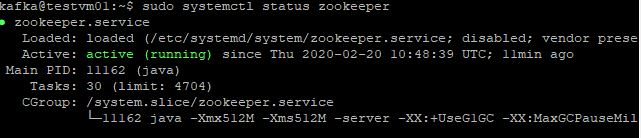
\includegraphics{images/StatusZookeeper}
	\caption{Status des Zookeeper-Dienstes nach dem Start}
	\label{img:StatusZookeeper}
\end{figure}

Für ein automatisches Starten des Dienstes nach einem Reboot führen Sie folgendes Kommando aus:

\smallskip

\begin{lstlisting}[language=Bash]
$ sudo systemctl enable zookeeper
\end{lstlisting}

Ab jetzt wird Zookeeper automatisch nach einem Neustart beim Hochfahren aller Systeme mit gestartet.

\pagebreak

\textbf{Kafka-Dienst starten:}

\bigskip

Führen Sie die gleichen Befehle für den Start des Kafka-Dienstes durch. Achten Sie darauf, dass Sie in allen Befehlen \glqq zookeeper\grqq durch \glqq kafka\grqq als Dienstbezeichnung ersetzen.

\smallskip

Überprüfen Sie mit dem \glqq status\grqq -Befehl, ob der Dienst richtig gestartet wurde. Der Output sollte so aussehen:

\begin{figure}[h]
	\centering
	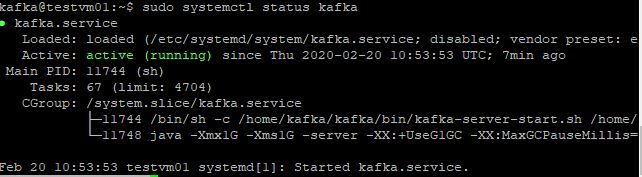
\includegraphics{images/StatusKafka}
	\caption{Status des Kafka-Dienstes nach dem Start}
	\label{img:StatusZookeeper}
\end{figure}

Nun sind Zookeeper und Kafka als Linux-Server-Dienst verfügbar ohne, dass ein Benutzer hierfür dauerhaft angemeldet sein muss.

\section{Schritt 5: Testen der Installation}

Um sicherzustellen, dass Kafka als Dienst korrekt läuft, wird eine \glqq HelloWorld\grqq -Nachricht produziert und konsumiert. Um eine Nachricht mittels Kafka zu versenden sind zwei Bestandteile nötig:

\begin{itemize}
\item Producer, welcher ein Topic registriert und Nachrichten produziert
\item Consumer, welcher Nachrichten aus dem Topic lesen kann
\end{itemize}

Hierfür werden die bei der Installation mitgelieferten Skripte im \glqq kafka\grqq -Verzeichnis benutzt.

Zuerst muss ein Topic erstellt werden. Das Topic heißt für Testzwecke \glqq Test\grqq.  Führen Sie folgenden Befehl aus:

\smallskip

\begin{lstlisting}[language=Bash]
$ ~/kafka/bin/kafka-topics.sh --create --zookeeper localhost:2181 --replication-factor 1 --partitions 1 --topic Test
\end{lstlisting}

Der Befehl benötigt den Zookeeper-Dienst mit dessen Portnummer (Standard-Port: 2181) als Argument, weil Zookeeper für die Verwaltung der Kafka-Instanzen benötigt wird. Ist das Topic erfolgreich erstellt worden, ist der Output auf der Kommandozeile \glqq Created topic Test.\grqq

\pagebreak

Um einen Producer zu starten, der als Nachricht \glqq HelloWorld\grqq produziert und dem Kafka-Dienst übergibt, führen Sie folgenden Befehl aus:

\smallskip

\begin{lstlisting}[language=Bash]
$ echo "Hello, World" | ~/kafka/bin/kafka-console-producer.sh --broker-list localhost:9092 --topic Test > /dev/null
\end{lstlisting}

Der Befehl produziert eine Nachricht für das Topic \glqq Test\grqq und übergibt die Nachricht an Kafka.

Der Consumer benötigt als Argument den Zookeeper Hostname und den Port (Standardport: 2181) und das Topic aus dem Nachrichten konsumiert werden sollen.

\smallskip

\begin{lstlisting}[language=Bash]
$ ~/kafka/bin/kafka-console-consumer.sh --bootstrap-server localhost:9092 --topic Test --from-beginning
\end{lstlisting}

Nach der Ausführung des Consumer-Skripts, sollte die Nachricht \glqq HelloWorld\grqq auf dem Bildschirm erfolgen. Ist das nicht der Fall, überprüfen Sie Ihre durchgeführten Schritte. Das Skript blockiert den Benutzerprozess, weil der Consumer weiterhin auf eintreffende Nachrichten wartet. Um das Skript abzubrechen verwenden Sie STR+C als Shortcut auf der Tastatur.

Kafka steht nun als Server-Dienst zur Verfügung und die Installation wurde durch einen Test erfolgreich validiert. Kafka kann für seine Einsatzbereiche ab jetzt vollständig verwendet werden.

\end{document}